\documentclass[aspectratio=169]{beamer}

\usepackage{clrscode}
\usepackage{graphicx}
\usepackage{booktabs}
\usepackage[most]{tcolorbox}
\usepackage{ragged2e}
\usepackage{amsmath, esint}
\usepackage[symbol]{footmisc}
\usepackage{tikz}
\usepackage{amsthm}
\usepackage{amstext}
\usepackage{amssymb}
\usepackage{minted}
\usepackage{xcolor}

\usetikzlibrary{backgrounds, positioning, arrows, scopes, shapes, shapes.misc, shapes.multipart}
\tikzset{
    cross/.style={cross out, draw=black, minimum size=2*(#1-\pgflinewidth), inner sep=0pt, outer sep=0pt},
    cross/.default={10pt},
    split/.style={rectangle split, rectangle split parts=7, draw, inner sep=0ex, rectangle split horizontal, minimum size=4ex},
    textstyle/.style={text height=1.5ex, text depth=.25ex}
}
\definecolor{LightGray}{gray}{0.975}
\hypersetup{colorlinks,linkcolor=,urlcolor=blue}

\usefonttheme{serif} 

\title[L5 DP]{Introduction to Algorithms \\ Lecture 5: Dynamic Programming (DP)}
\author{Prof. Charles E. Leiserson and Prof. Erik Demaine \\ Massachusetts Institute of Technology}
\date{\today}

%remove navigation symbols
\setbeamertemplate{navigation symbols}{}

\defbeamertemplate*{footline}{shadow theme}{
    \leavevmode
    \hbox{
        \begin{beamercolorbox}[
                wd =        0.33\paperwidth,
                ht =        2.5ex,
                dp =        1.125ex,
                leftskip =  0.3cm plus1fil,
                rightskip = 0.3cm
            ]{author in head/foot}
            \flushleft Analisis of Algorithms
        \end{beamercolorbox}
        \begin{beamercolorbox}[
                wd =        0.33\paperwidth,
                ht =        2.5ex,
                dp =        1.125ex,
                leftskip =  0.3cm plus1fil,
                rightskip = 0.3cm
            ]{author in head/foot}
            \insertshorttitle
        \end{beamercolorbox}
        \begin{beamercolorbox}[
                wd =        0.33\paperwidth,
                ht =        2.5ex,
                dp =        1.125ex,
                leftskip =  0.3cm plus1fil,
                rightskip = 0.3cm
            ]{title in head/foot}
            \hfill \insertframenumber\,/\,\inserttotalframenumber%
        \end{beamercolorbox}
    }
}

\AtBeginSection[]{
    \begin{frame}<beamer>
    \frametitle{Plan}
    \tableofcontents[currentsection]
    \end{frame}
}

\newcommand{\toRight}[1]{
    \begin{FlushRight}
        {\small #1}
    \end{FlushRight}
}

\begin{document}

\frame{\titlepage}

\begin{frame}{Introduction to Algorithms}
    \centering
    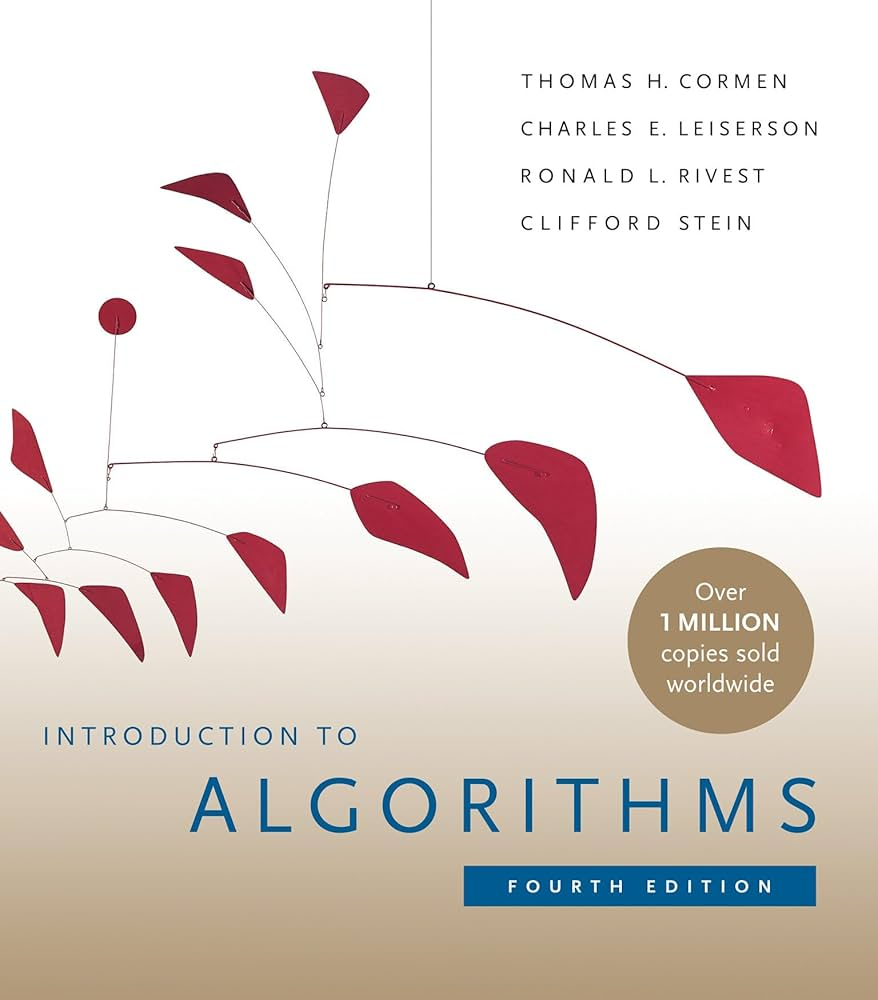
\includegraphics[width=0.35\textwidth]{figures/book_cover.jpg} \\
    \vspace{5mm}{
        \tiny
        Content has been extracted from \textit{Introduction to Algorithms}, Fourth Edition, by Cormen, Leiserson, Rivest, and Stein. MIT Press. 2022.\\
        Visit \url{https://mitpress.mit.edu/9780262046305/introduction-to-algorithms/}.\\
        Original slides from \textit{Introduction to Algorithms 6.046J/18.401J}, Fall 2005 Class by Prof. Charles Leiserson and Prof. Erik Demaine. MIT OpenCourseWare Initiative available at \url{https://ocw.mit.edu/courses/6-046j-introduction-to-algorithms-sma-5503-fall-2005/}.\\
    }
\end{frame}

\section{Dynamic Programming}

\begin{frame}{Dynamic Programming\footnote{\textit{Programming} in this context refers to a tabular method, not to writing computer code.} (DP)}
    \begin{itemize}
        \item Invented by Richard Bellman in 1950s.
        \item Desing technique, like Divide \& Conquer.
        \item Applies when the subproblems overlap (that is, when subproblems share subsubproblems).
        \item It solves each subsubproblem just once and then saves its answer in a table.
        \item DP typically applies to optimization problems:
        \begin{itemize}
            \item have many possible solutions.
            \item find a solution with the optimal (min or max) value.
            \item \textit{an} optimal solution, not \textit{the} optimal solution.
        \end{itemize}
    \end{itemize}
\end{frame}

\begin{frame}{DP notions}
    \begin{enumerate} \pause
        \item Characterize the structure of an optimal solution. \pause
        \item Recursively define the value of an optimal solution based on optimal solutions of subproblems. \pause
        \item Compute the value of an optimal solution in bottom-up fashion (recursion \& memoization). \pause
        \item Construct an optimal solution from the computed information. \pause
    \end{enumerate}
    \vspace{10mm}
    \centering
    \Large
    \textcolor{blue}{\textbf{DP}} = \textcolor{orange}{\textbf{Recursion}} + \textcolor{olive}{\textbf{Memoization}}
\end{frame}

\begin{frame}{DP notions}
    \centering
    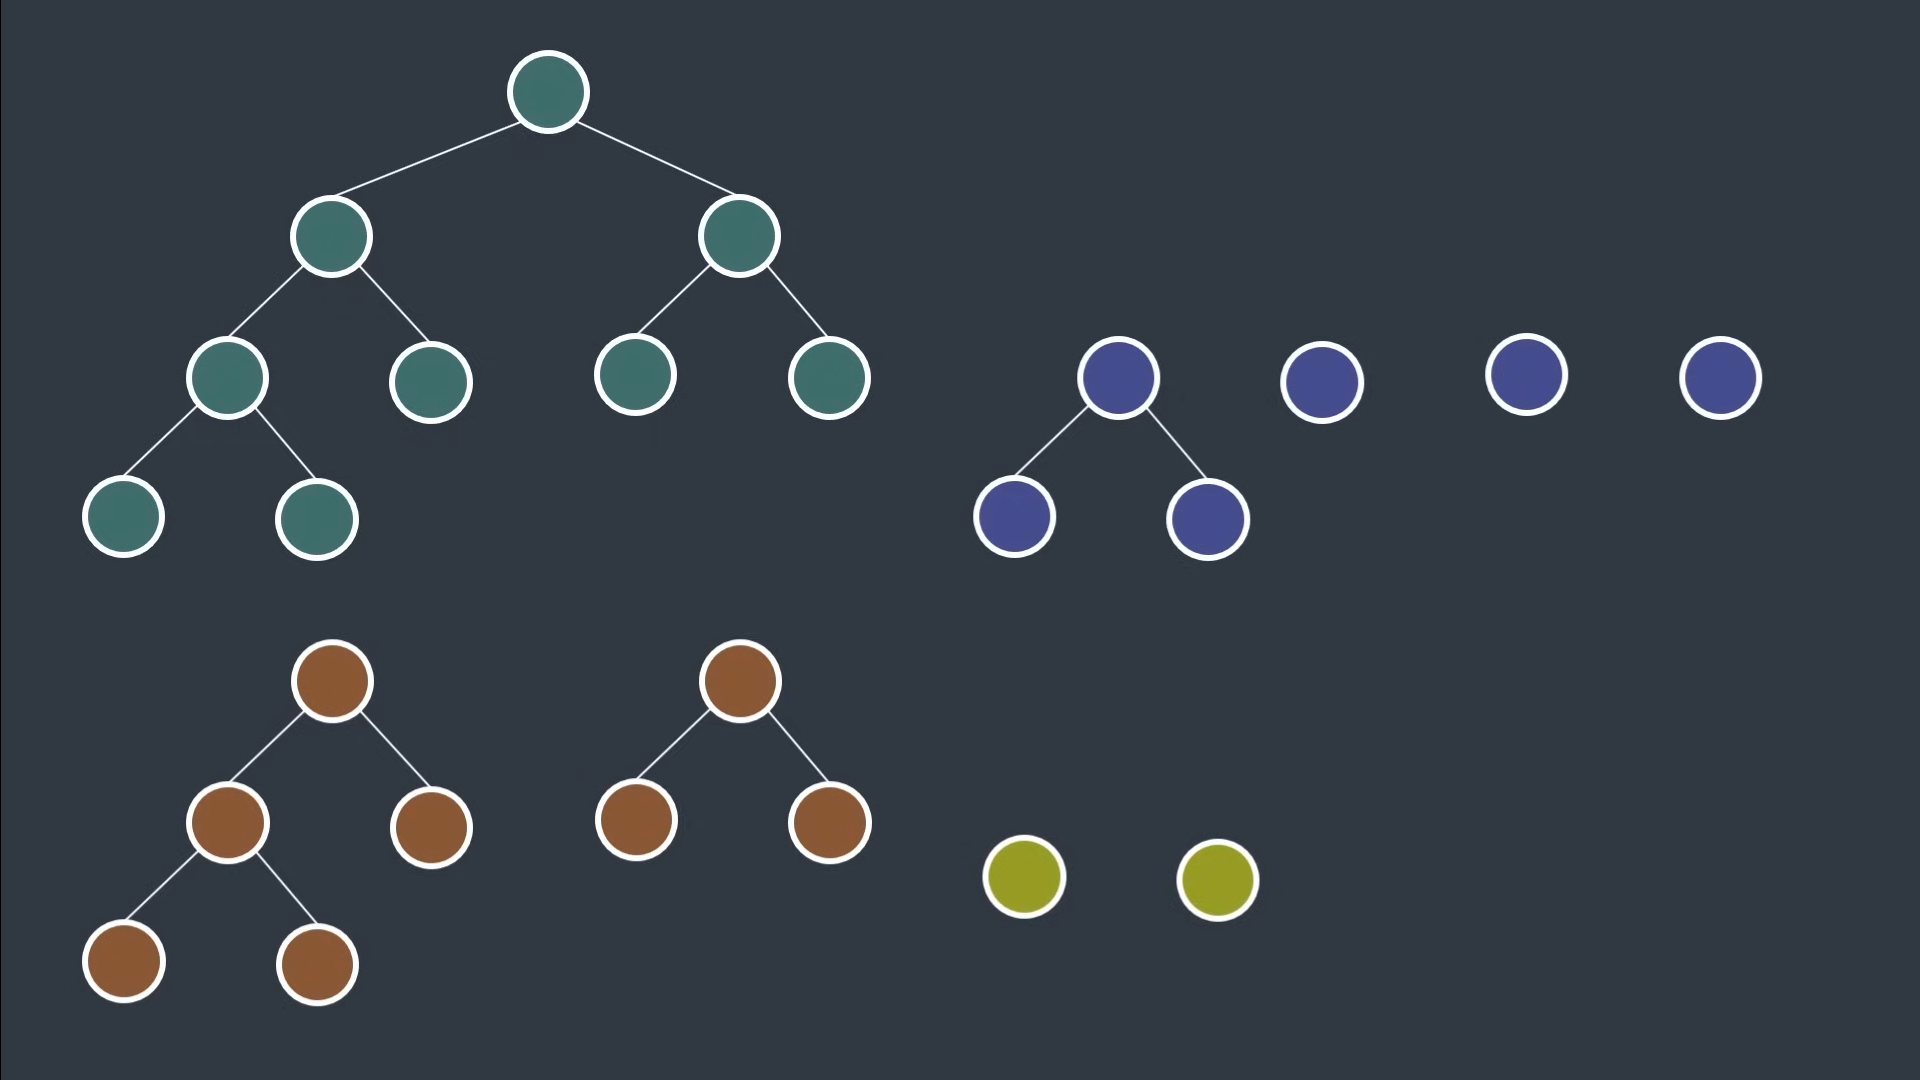
\includegraphics[width=0.95\textwidth]{figures/dp01.png}
\end{frame}

\section{N-th Fibonacci Number}

\begin{frame}{N-th Fibonacci Number\footnote{\scriptsize \textit{Mastering Dynamic Programming - How to solve any interview problem (Part 1)}. Tech With Nikola Channel, 2024. YouTube, available at \url{https://youtu.be/Hdr64lKQ3e4?si=ycTe-hoyfaICRWXt}}}
    Write a function that returns the n-th Fibonacci number.
    \begin{equation*}
        \begin{align*}
            F_1 &= F_2 = 1 \\
            F_n &= F_{n - 1} + F_{n - 2} \\
        \end{align*}
    \end{equation*}
    \centering
    \LARGE
    \begin{tabular}{| c | c | c | c | c | c | c | c |} \hline
        n & 1 & 2 & 3 & 4 & 5 & 6 & 7  \\ \hline
    $F_n$ & 1 & 1 & 2 & 3 & 5 & 8 & 13 \\ \hline
    \end{tabular}
\end{frame}

\begin{frame}[fragile]{Naive Approach}
    \begin{minted}
    [tabsize=4, obeytabs, frame=lines, framesep=2mm, baselinestretch=1.2, bgcolor=LightGray, fontsize=\scriptsize, linenos]{python}
    def fib(n):
        if n <= 2:
            result = 1
        else:
            result = fib(n - 1) + fib(n - 2)
        return result
    \end{minted}
    \pause
    \begin{minted}
    [tabsize=4, obeytabs, framesep=2mm, baselinestretch=1.2, bgcolor=LightGray, fontsize=\scriptsize]{text}
    print(fib(7))
    Output: 13
    print(fib(50))
    Output: ???
    \end{minted}
\end{frame}

\begin{frame}{Naive Approach}
    \centering
    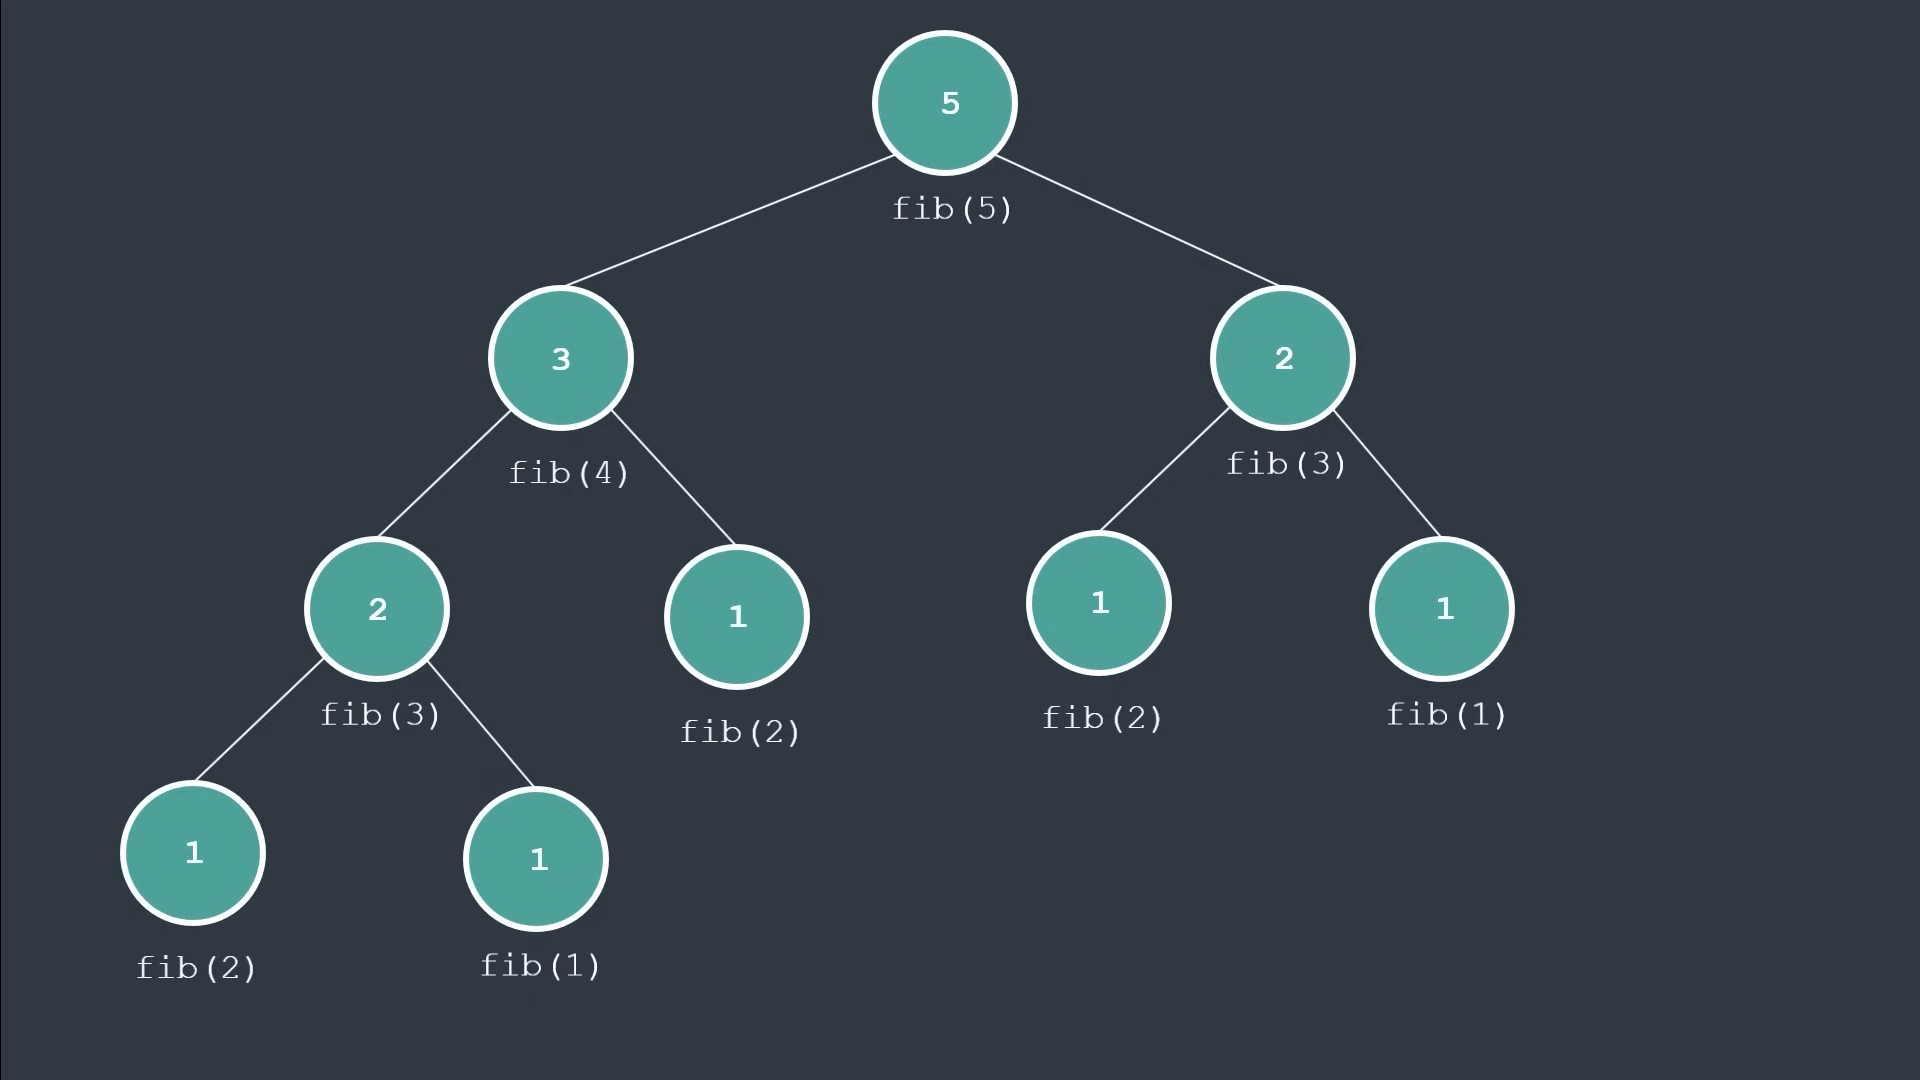
\includegraphics[width=0.95\textwidth]{figures/fb01.png}
\end{frame}
\begin{frame}{Naive Approach}
    \centering
    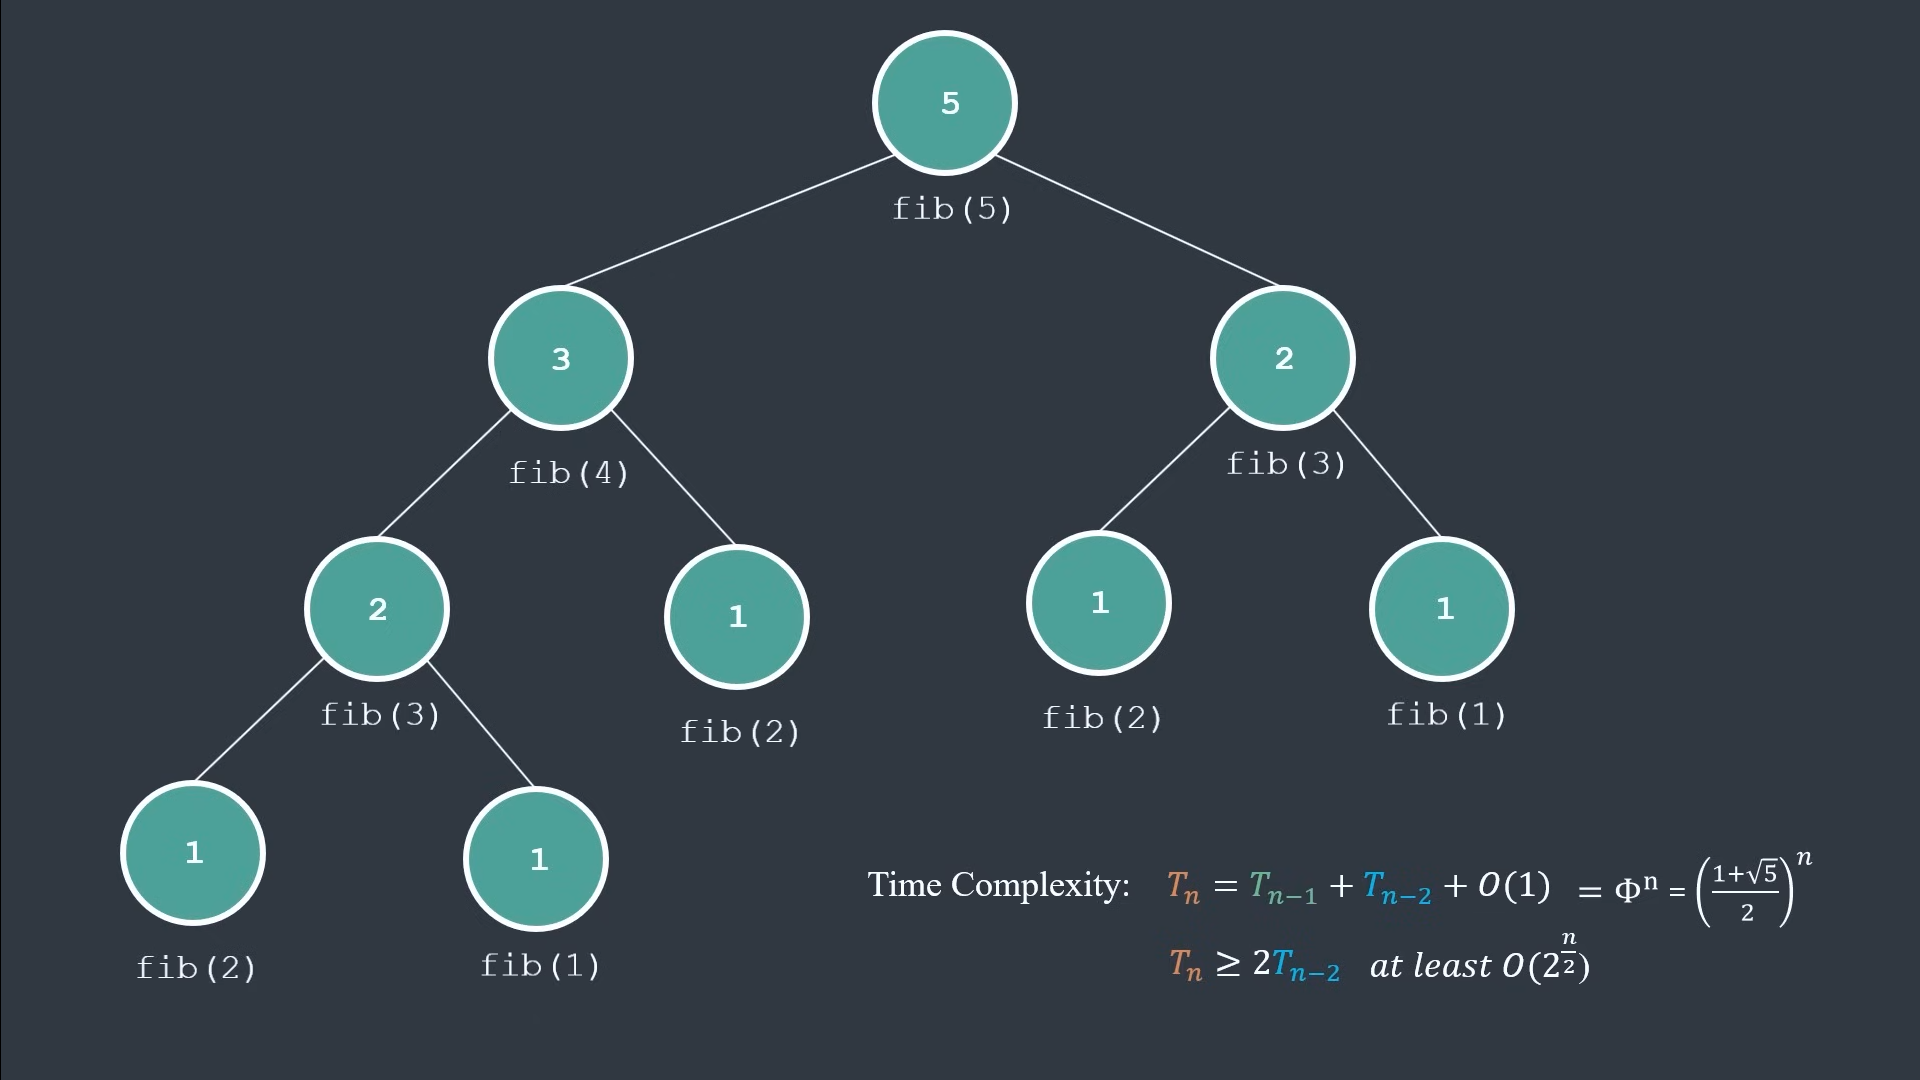
\includegraphics[width=0.95\textwidth]{figures/fb02.png}
\end{frame}
\begin{frame}{Naive Approach}
    \centering
    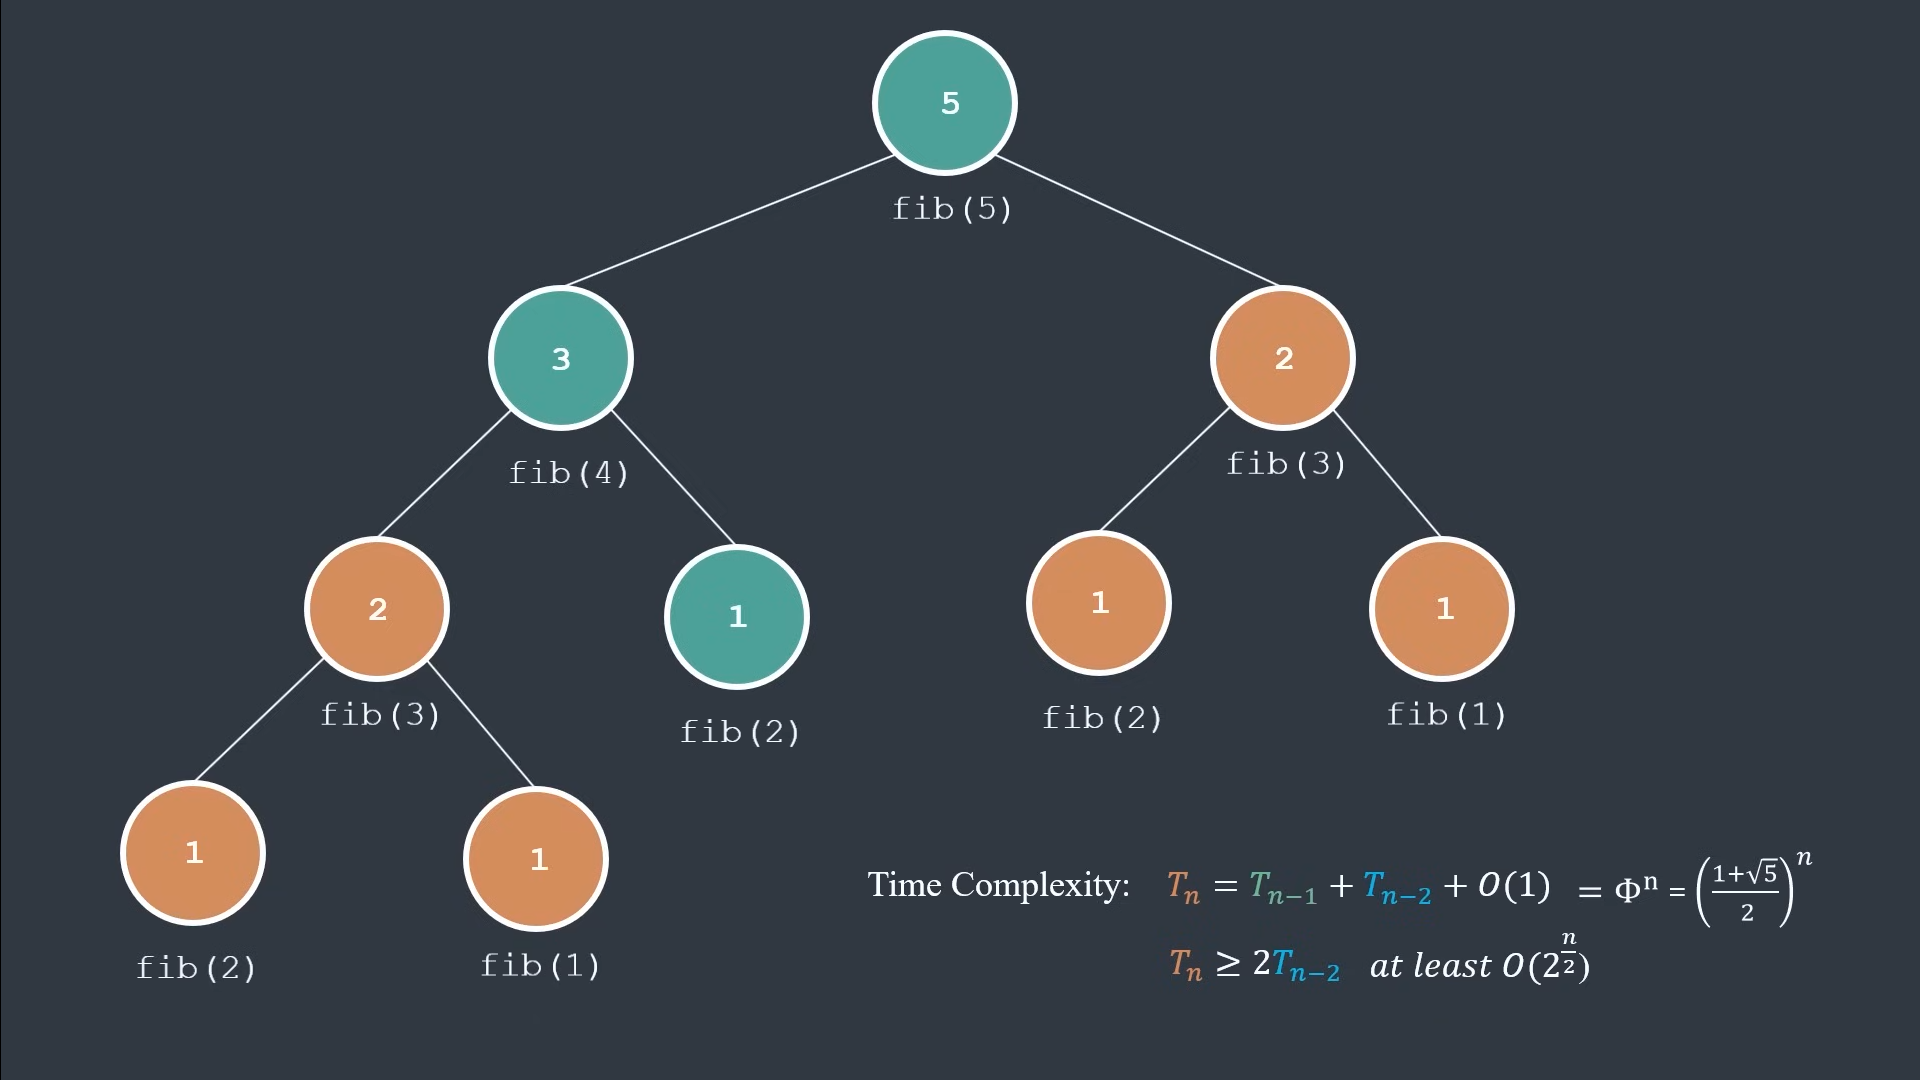
\includegraphics[width=0.95\textwidth]{figures/fb03.png}
\end{frame}
\begin{frame}{Naive Approach}
    \centering
    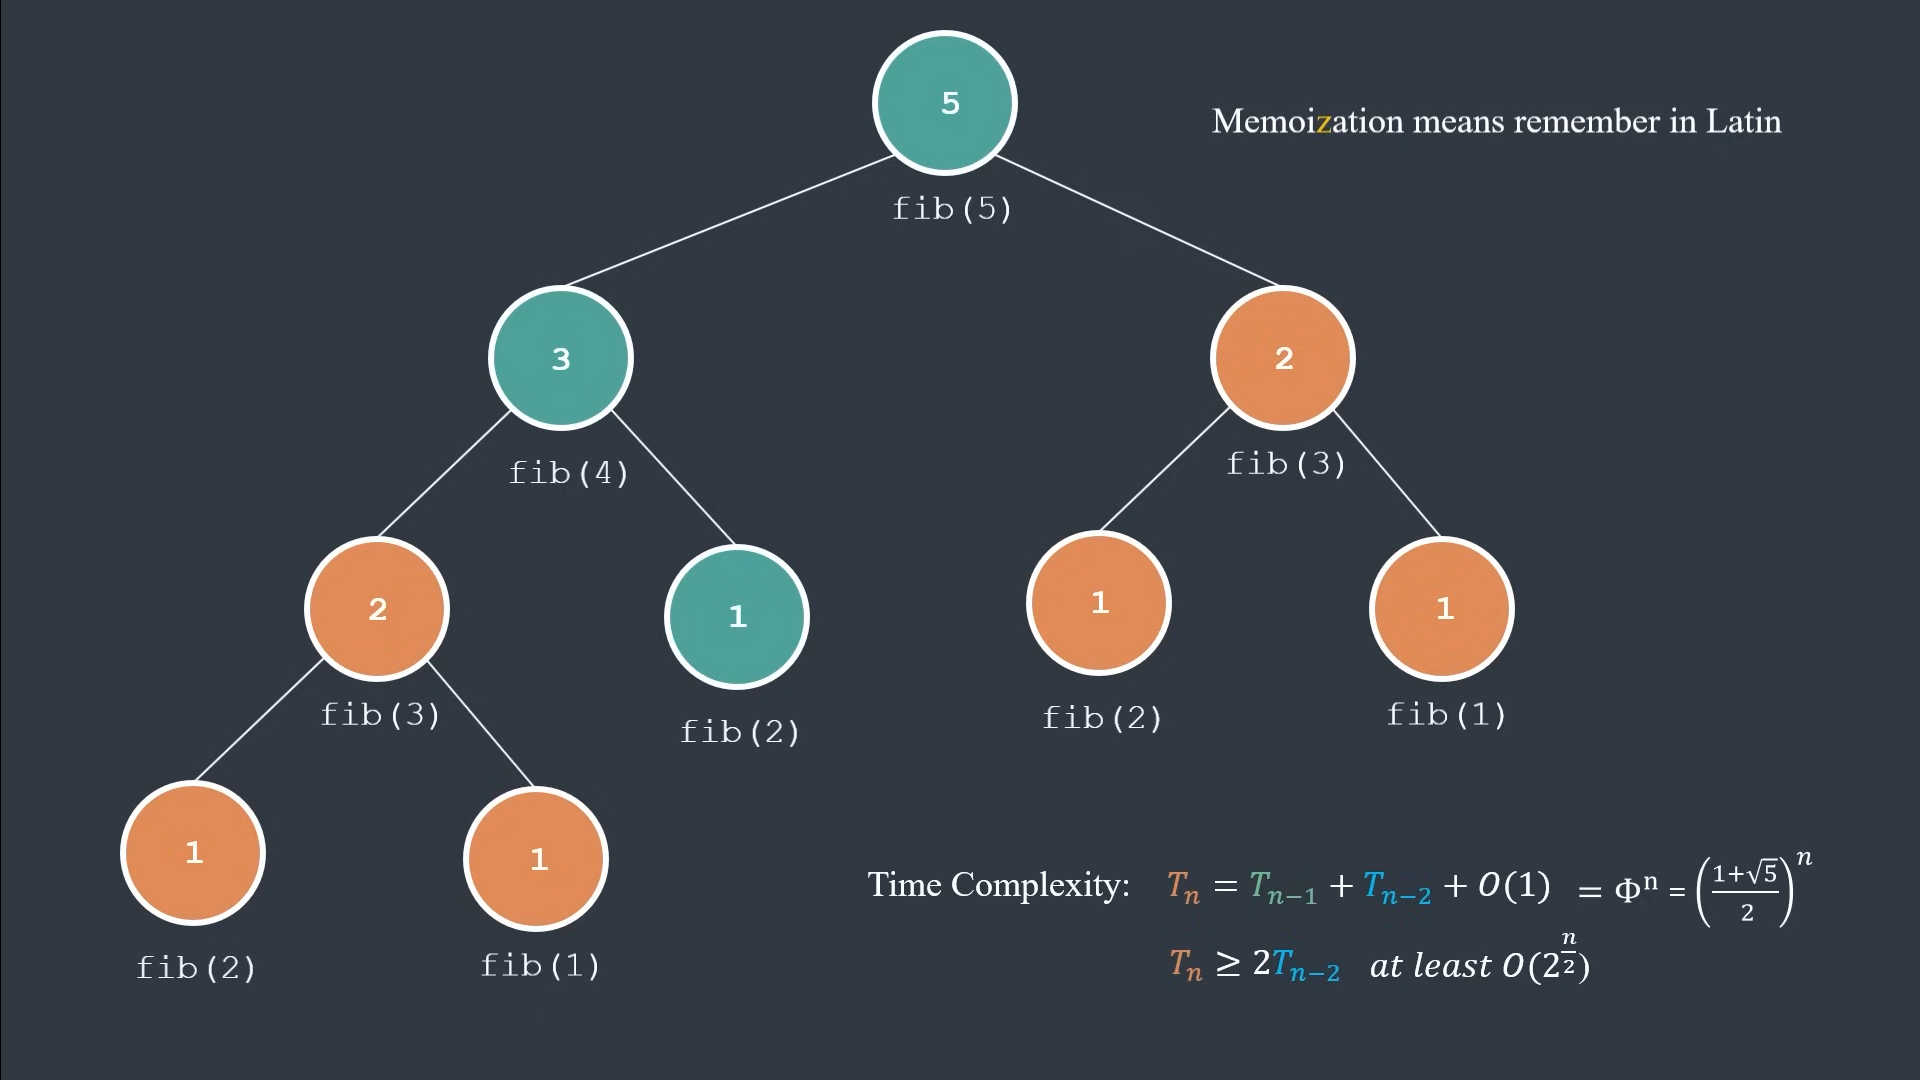
\includegraphics[width=0.95\textwidth]{figures/fb04.png}
\end{frame}

\begin{frame}[fragile]{Memoization Approach}
    \begin{minted}
    [tabsize=4, obeytabs, frame=lines, framesep=2mm, baselinestretch=1.2, bgcolor=LightGray, fontsize=\scriptsize, linenos]{python}
    memo = {} # adding a dictionary...
    def fib(n):
        if n in memo: # asking if n is in dict...
            return memo[n] # if so, we are done!
        if n <= 2:
            result = 1
        else:
            result = fib(n - 1) + fib(n - 2)
        return result
    \end{minted}
    \pause
    \begin{minted}
    [tabsize=4, obeytabs, framesep=2mm, baselinestretch=1.2, bgcolor=LightGray, fontsize=\scriptsize]{text}
    print(fib(7))
    Output: 13
    print(fib(50))
    Output: 12586269025
    \end{minted}
    \pause
    \Large
    Time Complexity: $O(n)$.
\end{frame}

\begin{frame}{ }
    \centering
    \LARGE
    \textcolor{blue}{\textbf{DP}} = \textcolor{orange}{\textbf{Recursion}} + \textcolor{olive}{\textbf{Memoization}}
\end{frame}

\begin{frame}[fragile]{Bottom-up Approach}
    \begin{minted}
    [tabsize=4, obeytabs, frame=lines, framesep=2mm, baselinestretch=1.2, bgcolor=LightGray, fontsize=\scriptsize, linenos]{python}
    def fib(n):
        memo = {}
        for i in range(1, n + 1):
            if i <= 2:
                result = 1
            else:
                result = memo[n - 1] + memo[n - 2]
            memo[i] = result
        return memo[n]
    \end{minted}
\end{frame}

\begin{frame}{ }
    \centering
    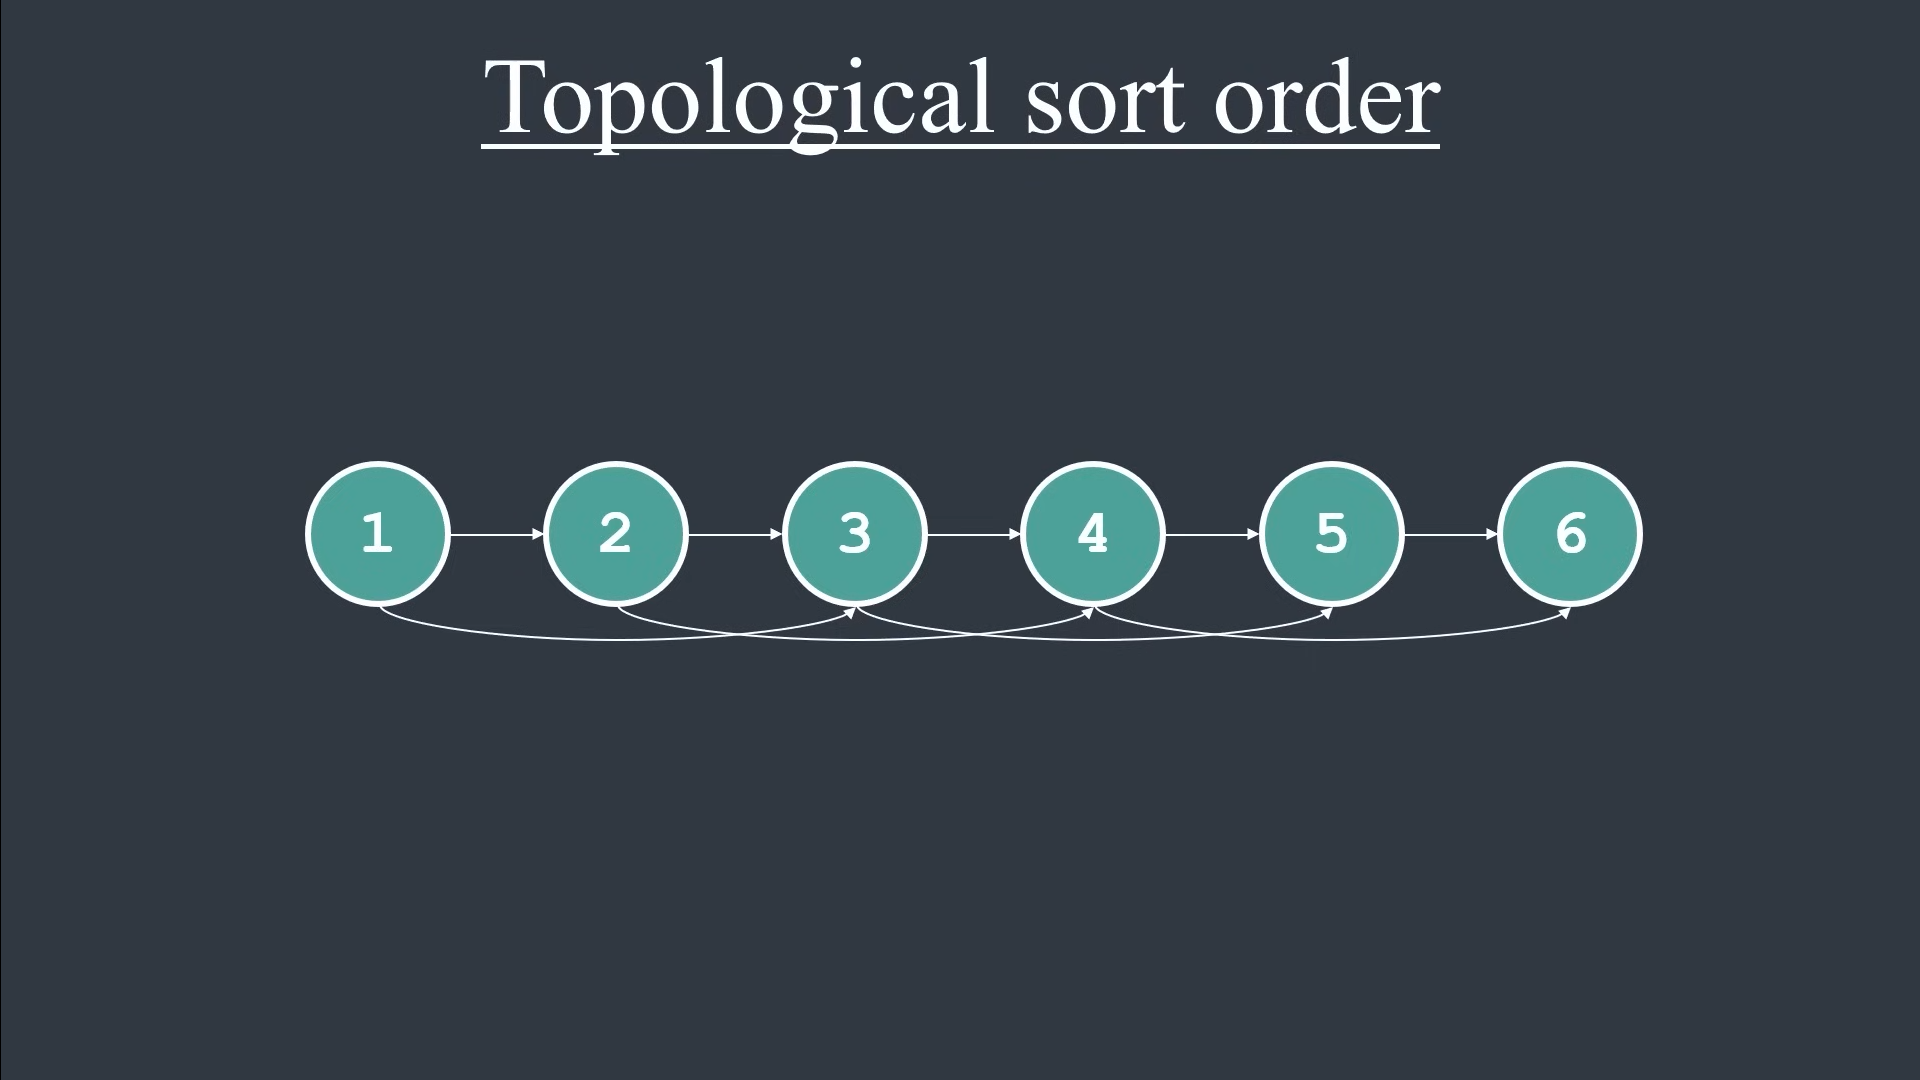
\includegraphics[width=\textwidth]{figures/topo.png}
\end{frame}

\section{Longest Palindromic Sequence}

\begin{frame}{Longest Palindromic Sequence}
    \begin{exampleblock}{Definition:}
        A palindrome is a string that is unchanged when reversed.
    \end{exampleblock}
    \begin{itemize}
     \item Examples: \texttt{radar}, \texttt{civic}, \texttt{t}, \texttt{bb}, \texttt{redder}.
     \item Given: A string $X[1 \ldots n]$, $n \geq 1$.
     \item To find: Longest palindrome that is a subsequence.
     \item Example: Given ``c h a r a c t e r''.
     \item Output: ``c a r a c''.
     \item Answer will be $\geq 1$ in length.
    \end{itemize}
\end{frame}

\begin{frame}[fragile]{Strategy}
    $L(i, j)$: length of longest palindromic subsequence of $X[i \ldots j]$ for $i \leq j$.
    \begin{minted}
    [tabsize=4, obeytabs, frame=lines, framesep=2mm, baselinestretch=1.2, bgcolor=LightGray, fontsize=\scriptsize, linenos]{python}
    def L(i, j):
        if i == j:
            return 1
        if X[i] == X[j]:
            if i + 1 == j:
                return 2
            else:
                return 2 + L(i + i, j - 1)
        else:
            return max( L(i + 1, j), L(i, j - 1) )
    \end{minted}
\end{frame}

\begin{frame}{Analysis}
    As written, program can run in exponential time: suppose all symbols $X[i]$ are distinct.
    \begin{equation*}
        \begin{align*}
            T(n) &= \text{running time on input of length } n \\
            T(n) &=
                    \begin{cases}
                        1         & n = 1 \\
                        2T(n - 1) & n > 1 \\
                    \end{cases} \\
                 &= 2^{n - 1}
        \end{align*}
    \end{equation*}
\end{frame}

\begin{frame}{What is missing?}
    \begin{itemize}
        \item Complexity is exponential... why? \pause
        \item We are still not completing all the DP notions...
        \item There is \textbf{recursion} but there is not \textbf{Memoization}... \pause
        \item Cache is missing!
        \item There is a single line of code that will fix it...
    \end{itemize}
\end{frame}

\begin{frame}{Understanding the Subproblems}
    The problem typically involves checking whether a substring of a given string is a palindrome. If the input string has a length of \( n \), then the natural way to define subproblems is:
    \begin{itemize}
        \item Consider all possible substrings $s[i:j]$ of the string.
        \item For each substring, determine whether it is a palindrome.
    \end{itemize}
\end{frame}

\begin{frame}{Counting the Subproblems}
    A substring is defined by two indices, \( i \) (starting index) and \( j \) (ending index), where \( 0 \leq i \leq j < n \). This means:
    \begin{itemize}
        \item \( i \) can take values from \( 0 \) to \( n-1 \).
        \item For each \( i \), \( j \) can take values from \( i \) to \( n-1 \).
    \end{itemize}
\end{frame}

\begin{frame}{Total Number of Subproblems}
    The total number of such \( (i, j) \) pairs (i.e., total subproblems) is given by the summation:
    \[
    \sum_{i=0}^{n-1} (n - i) = n + (n-1) + (n-2) + \dots + 1
    \]
    Using the formula for the sum of the first \( n \) natural numbers:
    \[
    \sum_{k=1}^{n} k = \frac{n(n+1)}{2}
    \]
    Thus, the number of subproblems is:
    \[
    n^2
    \]
\end{frame}

\begin{frame}{Formula for Computing the Complexity of a DP}
    \begin{large}
        \texttt{\# of subproblems} $\times$ \texttt{time to solve each subproblem}
    \end{large}
    \toRight{Given that smaller ones are already solved\footnote{lookup is $\Theta(1)$}.}
    \bigskip
    So,
    \begin{itemize}
        \item Given $n^2$ distinct subproblems...
        \item By solving each subproblem only once...
        \item Running time reduces to:
            {\LARGE
            $$
                \Theta(n^2) \cdot \Theta(1) = \Theta(n^2)
            $$
            }
    \end{itemize}
\end{frame}

\begin{frame}[fragile]{New Strategy}
    \begin{itemize}
        \item Memoize $L(i, j)$, hash inputs to get output value, and lookup hash table to see if the subproblem is already solved, else recurse.
    \end{itemize}

    \begin{minted}
    [tabsize=4, obeytabs, frame=lines, framesep=2mm, baselinestretch=1.2, bgcolor=LightGray, fontsize=\scriptsize, linenos]{python}
    def L(i, j):
        if i == j:
            return 1
        if X[i] == X[j]:
            if i + 1 == j:
                return 2
            else:
                return 2 + L(i + i, j - 1)
        else:
            return max( L(i + 1, j), L(i, j - 1) )
    \end{minted}
    \pause
    \begin{tikzpicture}[remember picture, overlay, node distance=3cm, text width=4cm, on grid, auto]
        \draw[orange, very thick, ->](5.35, 4.00) to [out=180,in=0](2.40, 4.575);
        \draw (7.50, 4.00) node[draw, orange, very thick, text=black]
            {\scriptsize
                Look at \verb|L[i, j]|
                and don't recurse if
                \verb|L[i, j]| is already
                computed.
            };
    \end{tikzpicture}
\end{frame}

\begin{frame}{Memoizing Vs. Iterating}
    \begin{enumerate}
        \item Memoizing uses a dictionary for $L(i, j)$ where value of $L$ is looked up by using $i, j$ as a key. Could just use a 2-D array here where null entries signify that the problem has not yet been solved.
        \item Can solve subproblems in order of increasing $j - i$ so smaller ones are solved first.
    \end{enumerate}
\end{frame}

\section{Longest Common Subsequence}

\begin{frame}{}
    \begin{itemize}
        \item Given two sequences $x[1 \cdots m]$ and $y[1 \cdots n]$, find a\footnote[2]{``a'' not ``the''} longest subsequence common to them both.
    \end{itemize} \pause
    \vspace{10mm}
    {\Huge x: \texttt{A B C B D A B}}\\
    \\
    {\Huge y: \texttt{B D C A B A}} \\
    \begin{itemize} \pause
        \item BDA ? \pause
        \item BDAB \pause
        \item BCAB \pause
        \item BCBA \pause
    \end{itemize}
    \texttt{LCS(x, y)} as notation \textbf{not function}...
\end{frame}

\begin{frame}{Brute-force LCS algorithm}
    \begin{itemize} \pause
        \item Check every subsequence of $x[1 \cdots m]$ to see if it is also a subsequence of $y[1 \cdots n]$.
    \end{itemize} \pause
    \begin{exampleblock}{Analysis}
        \begin{itemize}
            \item Checking = $O(n)$ time per subsequence.
            \item $2^m$ subsequences of $x$ (each bit-vector of length $m$ determines a distinct subsequence of $x$).
        \end{itemize}
        Worst-case running time $= O(n2^m)$ \pause \textcolor{red}{\textbf{Exponential time!}}
    \end{exampleblock}
\end{frame}

\begin{frame}{Towards a Better Algorithm}
    \begin{exampleblock}{Simplification:}
        \begin{enumerate}
            \item Look at the \textcolor{red}{\textit{length}} of a longest-common subsequence.
            \item Extend the algorithm to find the LCS itself.
        \end{enumerate}
    \end{exampleblock}
    \begin{itemize} \pause
        \item \textcolor{red}{\textbf{Notation:}} Denote the length of a sequence $s$ as $|s|$. \pause
        \item \textcolor{red}{\textbf{Strategy:}} Consider \textbf{prefixes} of $x$ and $y$:
            \begin{itemize}
                \item Define $c[i, j] = | LCS(x[1 \cdots i], y[1 \cdots j]) |$.
                \item Then, $c[m, n] = | LCS(x, y) |$.
            \end{itemize}
    \end{itemize}
\end{frame}

\begin{frame}{Recursive formulation}
    \begin{tcolorbox}[title=Theorem]
        \begin{equation*}
            \begin{align*}
                c[i, j] &=
                            \begin{cases}
                                0 & \text{ if } i = 0 \text{ or } j = 0 \text{, } \\
                                c[i - 1, j - 1] & \text{ if } x[i] = y[j] \text{, } \\
                                \max \{ c[i, j - 1], c[i - 1, j] \} & \text{ otherwise.}
                            \end{cases}
            \end{align*}
        \end{equation*}
    \end{tcolorbox}
    \textcolor{red}{\textbf{Proof:}} Case $x[i] = y[j] \ldots$ \\
    \\
    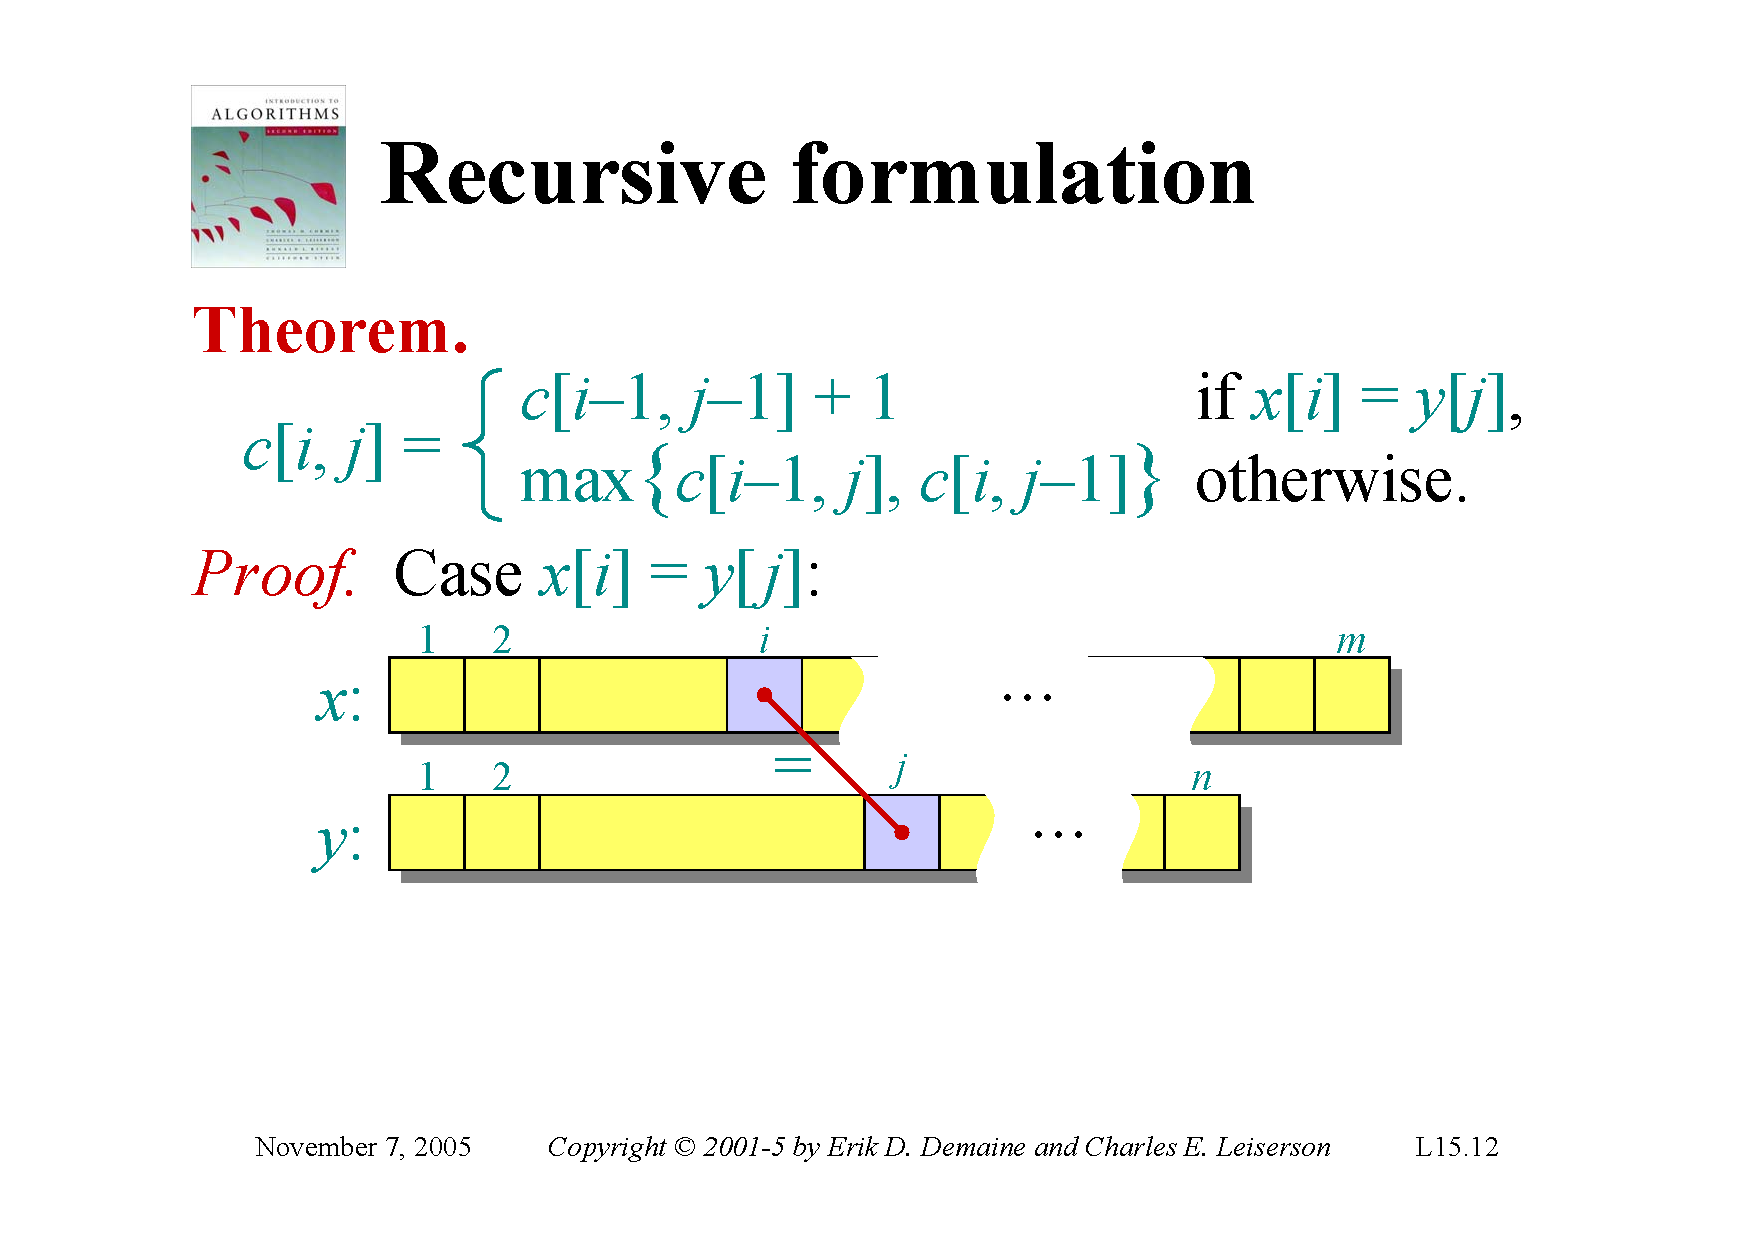
\includegraphics[width=\textwidth,trim=3cm 5cm 3cm 10.50cm, clip]{figures/proof01.pdf}
\end{frame}

\begin{frame}{Recursive formulation}
    \textcolor{red}{\textbf{Proof:}} Case $x[i] = y[j] \ldots$ \\
    \\
    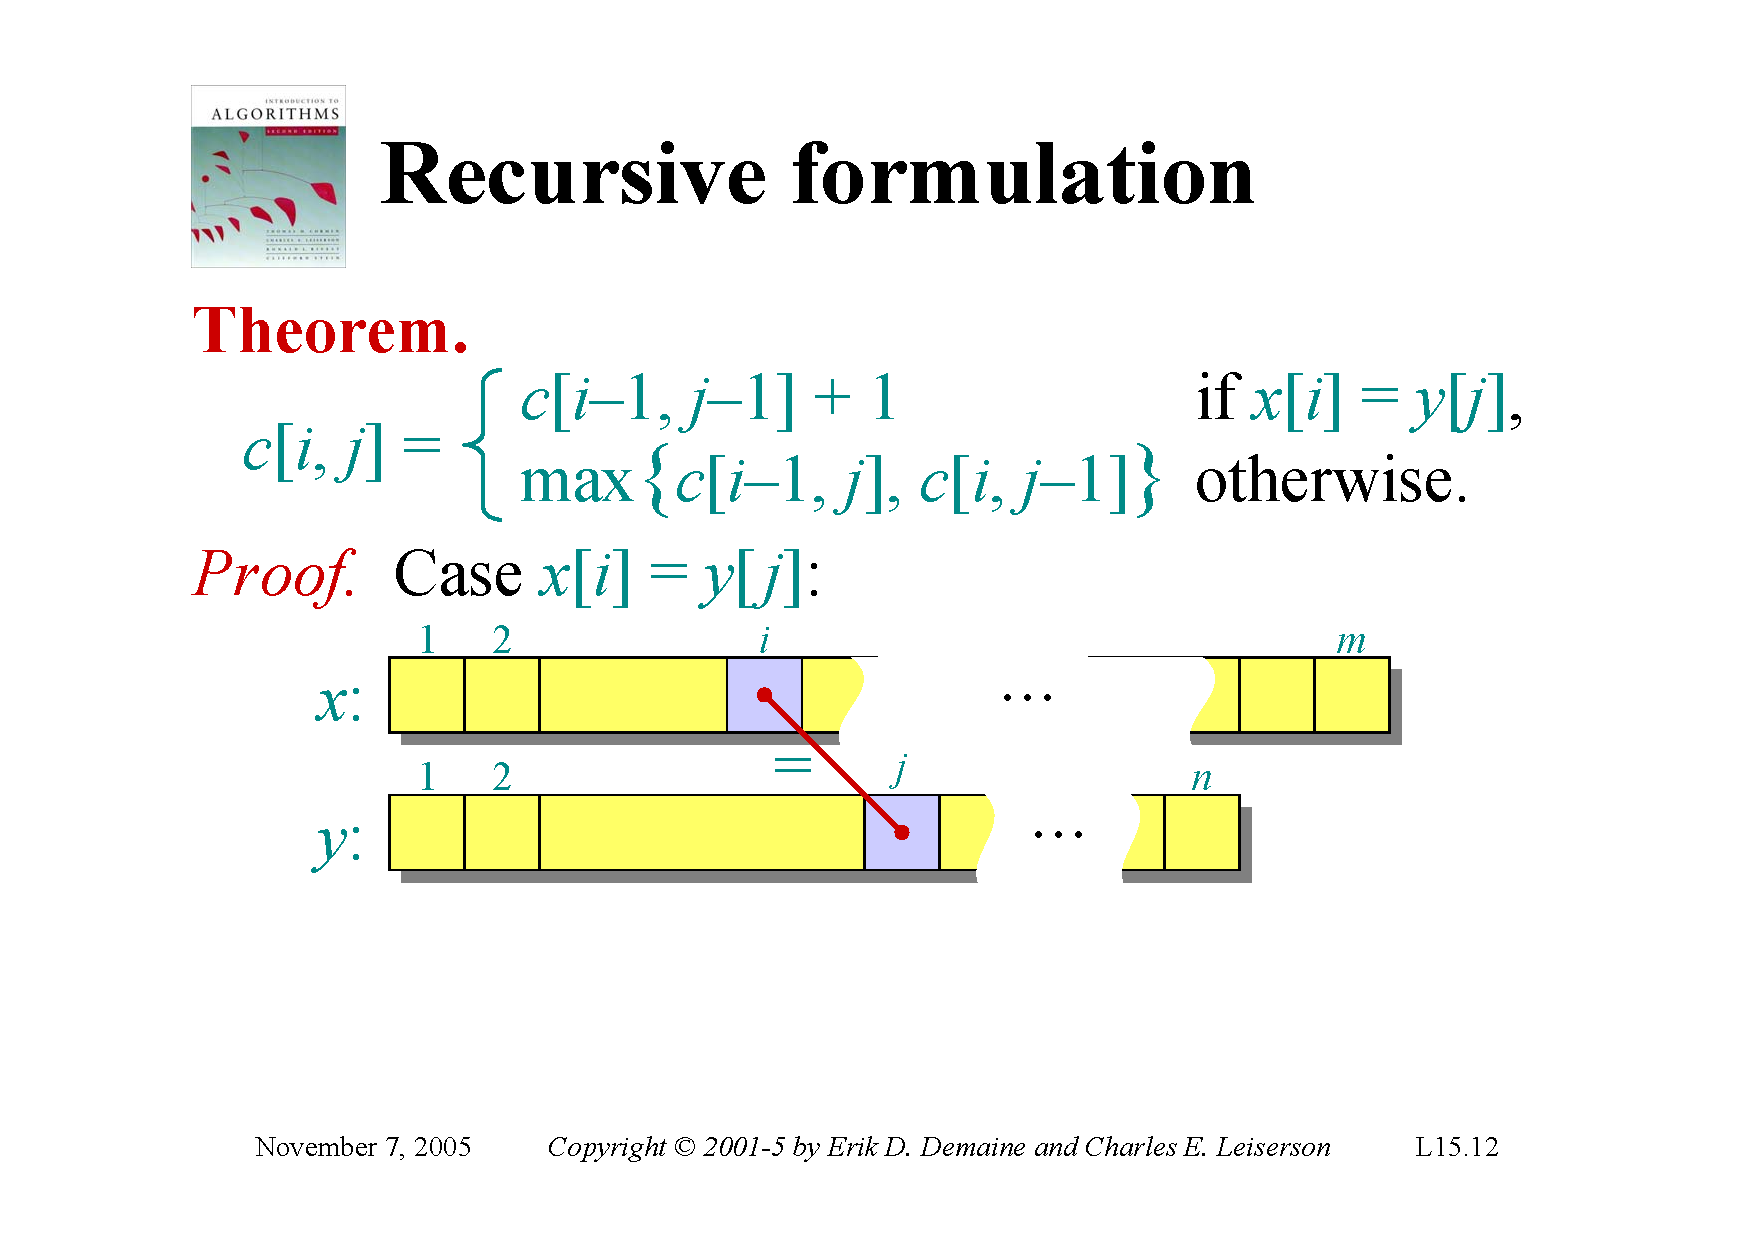
\includegraphics[width=\textwidth,trim=3cm 5cm 3cm 10.50cm, clip]{figures/proof01.pdf}
    \begin{itemize}
        \item Let $z[1 \cdots k] = LCS(x[1 \cdots i], y[1 \cdots j])$, where $c[i, j] = k$. \pause
        \item Then, $z[k] =$ \pause $x[i] ( = y[j])$\pause, or else $z$ could be extended. \pause
        \item Thus, $z[1 \cdots k–1]$ is CS of $x[1 \cdots i - 1]$ and $y[1 \cdots j - 1]$.
    \end{itemize}
\end{frame}

\begin{frame}{Step-by-Step Example of LCS Algorithm}
    We will use the dynamic programming (DP) approach to compute the LCS for the following strings:\\

    {\Huge X = ``ACDBE''} \\
    \\
    {\Huge Y = ``ABCDE''}
\end{frame}

\begin{frame}{Step 1: Create a DP Table}
    \begin{itemize}
        \item We construct a $(m+1) \times (n+1)$ table, where $m$ and $n$ are the lengths of $X$ and $Y$, respectively. The table will store the LCS length at each step.
        \item \textbf{Initial Table (before computation):} We initialize the first row and first column with 0s (LCS of empty strings is 0).
    \end{itemize}
\end{frame}

\begin{frame}{Step 1: Create a DP Table}
    \centering
    \begin{tabular}{|c|c|c|c|c|c|c|} \hline
                      & $\varnothing$ & A & B & C & D & E \\ \hline
        $\varnothing$ &        0      & 0 & 0 & 0 & 0 & 0 \\ \hline
               A      &        0      &   &   &   &   &   \\ \hline
               C      &        0      &   &   &   &   &   \\ \hline
               D      &        0      &   &   &   &   &   \\ \hline
               B      &        0      &   &   &   &   &   \\ \hline
               E      &        0      &   &   &   &   &   \\ \hline
    \end{tabular}
\end{frame}

\begin{frame}{Step 2: Fill the DP Table Using Recurrence}
    We iterate over each character of $X$ and $Y$ and apply the recurrence:
    \begin{equation*}
        \begin{align*}
            L[i, j] &=
                        \begin{cases}
                            L[i - 1, j - 1] + 1 & \text{ if } x[i] = y[j] \text{, } \\
                            \max \{ c[i, j - 1], c[i - 1, j] \} & \text{ otherwise.}
                        \end{cases}
        \end{align*}
    \end{equation*}
    \centering
    \begin{tabular}{|c|c|c|c|c|c|c|} \hline
                      & $\varnothing$ & A & B & C & D & E \\ \hline
        $\varnothing$ &        0      & 0 & 0 & 0 & 0 & 0 \\ \hline
               A      &        0      &   &   &   &   &   \\ \hline
               C      &        0      &   &   &   &   &   \\ \hline
               D      &        0      &   &   &   &   &   \\ \hline
               B      &        0      &   &   &   &   &   \\ \hline
               E      &        0      &   &   &   &   &   \\ \hline
    \end{tabular}
\end{frame}

\begin{frame}{Step 2: Fill the DP Table Using Recurrence}{Filling the table...}
    \vspace{-10mm}
    \scriptsize
    \begin{equation*}
        \begin{align*}
            L[i, j] &=
                        \begin{cases}
                            L[i - 1, j - 1] + 1 & \text{ if } x[i] = y[j] \text{, } \\
                            \max \{ c[i, j - 1], c[i - 1, j] \} & \text{ otherwise.}
                        \end{cases}
        \end{align*}
    \end{equation*}
    \begin{itemize}
        \item Compare `A' ($X[1]$) with each character in $Y$.
        \item `A' matches `A' $\longrightarrow L[1,1] = L[0,0] + 1 = 1$.
        \item Other cells get the max of left or top.
    \end{itemize}
    \vspace{6mm}
    \normalsize
    \centering
    \begin{tabular}{|c|c|c|c|c|c|c|} \hline
                      & $\varnothing$ & A & B & C & D & E \\ \hline
        $\varnothing$ &        0      & 0 & 0 & 0 & 0 & 0 \\ \hline
               A      &        0      & 1 & 1 & 1 & 1 & 1 \\ \hline
               C      &        0      &   &   &   &   &   \\ \hline
               D      &        0      &   &   &   &   &   \\ \hline
               B      &        0      &   &   &   &   &   \\ \hline
               E      &        0      &   &   &   &   &   \\ \hline
    \end{tabular}
\end{frame}

\begin{frame}{Step 2: Fill the DP Table Using Recurrence}{Filling the table...}
    \vspace{-10mm}
    \scriptsize
    \begin{equation*}
        \begin{align*}
            L[i, j] &=
                        \begin{cases}
                            L[i - 1, j - 1] + 1 & \text{ if } x[i] = y[j] \text{, } \\
                            \max \{ c[i, j - 1], c[i - 1, j] \} & \text{ otherwise.}
                        \end{cases}
        \end{align*}
    \end{equation*}
    \begin{itemize}
        \item Compare `C' ($X[2]$) with each character in $Y$.
        \item `C' matches `C' $\longrightarrow L[2,3] = L[1,2] + 1 = 2$.
        \item Other cells get the max of left or top.
    \end{itemize}
    \vspace{6mm}
    \normalsize
    \centering
    \begin{tabular}{|c|c|c|c|c|c|c|} \hline
                      & $\varnothing$ & A & B & C & D & E \\ \hline
        $\varnothing$ &        0      & 0 & 0 & 0 & 0 & 0 \\ \hline
               A      &        0      & 1 & 1 & 1 & 1 & 1 \\ \hline
               C      &        0      & 1 & 1 & 2 & 2 & 2 \\ \hline
               D      &        0      &   &   &   &   &   \\ \hline
               B      &        0      &   &   &   &   &   \\ \hline
               E      &        0      &   &   &   &   &   \\ \hline
    \end{tabular}
\end{frame}

\begin{frame}{Step 2: Fill the DP Table Using Recurrence}{Filling the table...}
    \vspace{-10mm}
    \scriptsize
    \begin{equation*}
        \begin{align*}
            L[i, j] &=
                        \begin{cases}
                            L[i - 1, j - 1] + 1 & \text{ if } x[i] = y[j] \text{, } \\
                            \max \{ c[i, j - 1], c[i - 1, j] \} & \text{ otherwise.}
                        \end{cases}
        \end{align*}
    \end{equation*}
    \begin{itemize}
        \item Compare `D' ($X[3]$) with each character in $Y$.
        \item `D' matches `D' $\longrightarrow L[3,4] = L[2,3] + 1 = 3$.
        \item Other cells get the max of left or top.
    \end{itemize}
    \vspace{6mm}
    \normalsize
    \centering
    \begin{tabular}{|c|c|c|c|c|c|c|} \hline
                      & $\varnothing$ & A & B & C & D & E \\ \hline
        $\varnothing$ &        0      & 0 & 0 & 0 & 0 & 0 \\ \hline
               A      &        0      & 1 & 1 & 1 & 1 & 1 \\ \hline
               C      &        0      & 1 & 1 & 2 & 2 & 2 \\ \hline
               D      &        0      & 1 & 1 & 2 & 3 & 3 \\ \hline
               B      &        0      &   &   &   &   &   \\ \hline
               E      &        0      &   &   &   &   &   \\ \hline
    \end{tabular}
\end{frame}

\begin{frame}{Step 2: Fill the DP Table Using Recurrence}{Filling the table...}
    \vspace{-10mm}
    \scriptsize
    \begin{equation*}
        \begin{align*}
            L[i, j] &=
                        \begin{cases}
                            L[i - 1, j - 1] + 1 & \text{ if } x[i] = y[j] \text{, } \\
                            \max \{ c[i, j - 1], c[i - 1, j] \} & \text{ otherwise.}
                        \end{cases}
        \end{align*}
    \end{equation*}
    \begin{itemize}
        \item Compare `B' ($X[4]$) with each character in $Y$.
        \item `B' matches `B' $\longrightarrow L[4,2] = L[3,1] + 1 = 2$.
        \item Other cells get the max of left or top.
    \end{itemize}
    \vspace{6mm}
    \normalsize
    \centering
    \begin{tabular}{|c|c|c|c|c|c|c|} \hline
                      & $\varnothing$ & A & B & C & D & E \\ \hline
        $\varnothing$ &        0      & 0 & 0 & 0 & 0 & 0 \\ \hline
               A      &        0      & 1 & 1 & 1 & 1 & 1 \\ \hline
               C      &        0      & 1 & 1 & 2 & 2 & 2 \\ \hline
               D      &        0      & 1 & 1 & 2 & 3 & 3 \\ \hline
               B      &        0      & 1 & 2 & 2 & 3 & 3 \\ \hline
               E      &        0      &   &   &   &   &   \\ \hline
    \end{tabular}
\end{frame}

\begin{frame}{Step 2: Fill the DP Table Using Recurrence}{Filling the table...}
    \vspace{-10mm}
    \scriptsize
    \begin{equation*}
        \begin{align*}
            L[i, j] &=
                        \begin{cases}
                            L[i - 1, j - 1] + 1 & \text{ if } x[i] = y[j] \text{, } \\
                            \max \{ c[i, j - 1], c[i - 1, j] \} & \text{ otherwise.}
                        \end{cases}
        \end{align*}
    \end{equation*}
    \begin{itemize}
        \item Compare `E' ($X[5]$) with each character in $Y$.
        \item `E' matches `E' $\longrightarrow L[5,5] = L[4,4] + 1 = 4$.
        \item Other cells get the max of left or top.
    \end{itemize}
    \vspace{6mm}
    \normalsize
    \centering
    \begin{tabular}{|c|c|c|c|c|c|c|} \hline
                      & $\varnothing$ & A & B & C & D & E \\ \hline
        $\varnothing$ &        0      & 0 & 0 & 0 & 0 & 0 \\ \hline
               A      &        0      & 1 & 1 & 1 & 1 & 1 \\ \hline
               C      &        0      & 1 & 1 & 2 & 2 & 2 \\ \hline
               D      &        0      & 1 & 1 & 2 & 3 & 3 \\ \hline
               B      &        0      & 1 & 2 & 2 & 3 & 3 \\ \hline
               E      &        0      & 1 & 2 & 2 & 3 & 4 \\ \hline
    \end{tabular}
\end{frame}

\begin{frame}{Step 3: Extract the LCS}
    \begin{itemize}
        \item The \textbf{LCS} length is in the bottom-right cell, $L[5,5] = 4$.
        \item To trace back the \textbf{LCS}, we start from $L[5,5]$ and follow:
        \begin{itemize}
            \item If $X[i] = Y[j]$, include it in the \textbf{LCS}.
            \item Otherwise, move to the maximum value from the left or top.
        \end{itemize}
    \end{itemize}

    Tracing Back from L[5,5]:
    \begin{enumerate}
        \item E ($X[5] = Y[5]$) $\longrightarrow$ Add `E'
        \item D ($X[3] = Y[4]$) $\longrightarrow$ Add `D'
        \item C ($X[2] = Y[3]$) $\longrightarrow$ Add `C'
        \item A ($X[1] = Y[1]$) $\longrightarrow$ Add `A'
    \end{enumerate}
    Thus, the LCS = ``ACDE''.
\end{frame}

\begin{frame}{Longest Common Subsequence -- Formal Steps of DP}{Step 1: Characterizing a longest common subsequence}
    \begin{itemize}
        \item You can solve the LCS problem with a brute-force approach:
        \begin{enumerate}
            \item Enumerate all subsequences of X.
            \item Check each subsequence to see weather it is also subsequence of Y.
            \item Keep track of the longest subsequence.
        \end{enumerate}
        \item Because X has $2^m$ possible subsequence, time is exponential and, ergo, impractical.
    \end{itemize}
\end{frame}

\begin{frame}{Longest Common Subsequence -- Formal Steps of DP}{Step 1: Characterizing a longest common subsequence}
    \begin{itemize}
        \item The LCS problem has an optimal-substructure property.
        \item the natural classes of subproblems correspond to pairs of \textit{``prefixes''} of the two input sequences:
        \begin{itemize}
            \item Given the sequence $X=\langle x_1, x_2, \ldots, x_m\rangle$:
            \item We can define the \textit{i-th} \textbf{prefix} of X, for $i = 0, 1, \ldots, m$, as $X_i = \langle x_1, x_2, \ldots, x_i\rangle$.
            \item For instance, if $X = \langle A B C B D A B \rangle$, then $X_4 = \langle A B C B \rangle$ and $X_0$ in the empty sequence.
        \end{itemize}
    \end{itemize}
\end{frame}

\begin{frame}{Longest Common Subsequence -- Formal Steps of DP}{Step 1: Characterizing a longest common subsequence}
    \begin{tcolorbox}[title=Theorem 14.1 (Optimal substructure of an LCS)]
        Let $X=\langle x_1, x_2, \ldots, x_m\rangle$ and $Y=\langle y_1, y_2, \ldots, y_n\rangle$ be sequences, and let $Z=\langle z_1, z_2, \ldots, z_k\rangle$ be any LCS of $X$ and $Y$.
        \begin{enumerate}
            \item If $x_m = y_n$, then $z_k = x_m = y_n$ and $Z_{k - 1}$ is a LCS of $X_{m-1}$ and $Y_{n-1}$. \pause
            \item If $x_m \neq y_n$ and $z_k \neq x_m$, then $Z$ is a LCS of $X_{m-1}$ and $Y$. \pause
            \item If $x_m \neq y_n$ and $z_k \neq y_n$, then $Z$ is a LCS of $X$ and $Y_{n-1}$.
        \end{enumerate}
    \end{tcolorbox}
    \toRight{Proof in CLRS page 395.}
\end{frame}

\begin{frame}{Longest Common Subsequence -- Formal Steps of DP}{Step 1: Characterizing a longest common subsequence}
    \begin{itemize}
        \item Theorem 14.1 says that an LCS of two sequences contains within it an LCS of prefixes of the two sequences.
        \item Thus, the LCS problem has an optimal-substructure property.
        \item A recursive solution also has the overlapping-subproblems property (as we’ll see in a moment).
    \end{itemize}
\end{frame}

\begin{frame}{Longest Common Subsequence -- Formal Steps of DP}{Step 2: A recursive solution}
    \begin{itemize}
        \item To find an LCS of $X$ and $Y$, you might need to find the LCSs of $X$ and $Y_{n-1}$ and of $X_{m-1}$ and $Y$ (overlapping property).
        \item Each of these subproblems has the subsubproblem of finding an LCS of $X_{m-1}$ and $Y_{n-1}$.
        \item Many other subproblems share subsubproblems.
    \end{itemize}
\end{frame}

\begin{frame}{Longest Common Subsequence -- Formal Steps of DP}{Step 2: A recursive solution}
    The optimal substructure of the LCS problem gives the recursive formula:
    \begin{equation*}
        \begin{align*}
            c[i, j] &=
                        \begin{cases}
                            0 & \text{ if } i = 0 \text{ or } j = 0 \text{, } \\
                            c[i - 1, j - 1] + 1 & \text{ if } i,j > 0 \text{ and } x[i] = y[j] \text{, } \\
                            \max \{ c[i, j - 1], c[i - 1, j] \} & \text{ if } i,j > 0 \text{ and } x[i] \neq y[j].
                        \end{cases}
        \end{align*}
    \end{equation*}
    \begin{itemize} \pause
        \item Define $c[i,j] =$ length of LCS of $X_i$ and $Y_j$. Want $c[m,n]$. \pause
        \item Again, could write a recursive algorithm based on this formulation, but...
    \end{itemize}
\end{frame}

\begin{frame}{Longest Common Subsequence -- Formal Steps of DP}{Step 2: A recursive solution}
    \begin{itemize}
        \item Try with $X=\langle a,t,o,m \rangle$ and $Y=\langle a,n,t \rangle$.
        \item Numbers in nodes are values of $i, j$ in each recursive call.
        \item Dashed lines indicate subproblems already computed.
    \end{itemize}
    \centering
    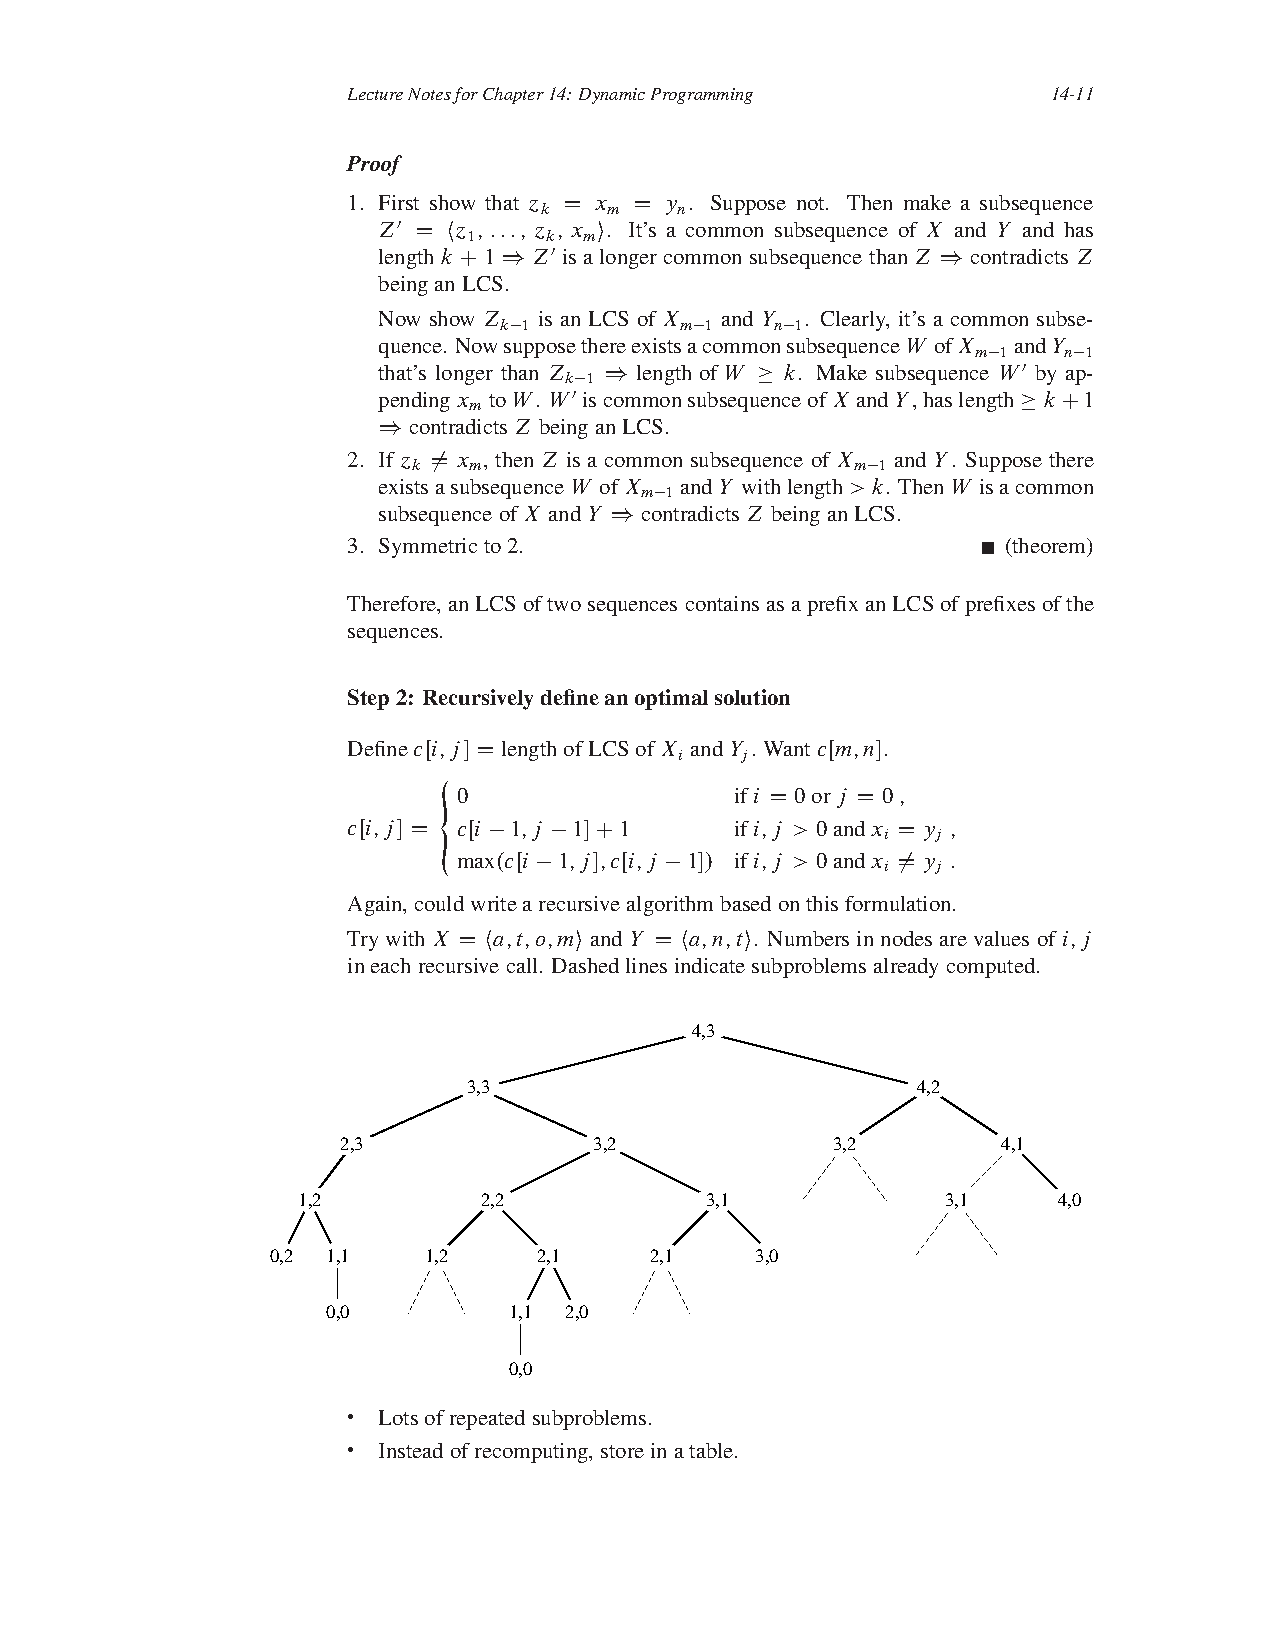
\includegraphics[width=\textwidth,clip,trim=4cm 4.25cm 3cm 17cm]{figures/overlapping.pdf}
    \vspace{-10mm}
    \toRight{\tiny Lots of repeated subproblems. Instead of recomputing, store in a table.}
\end{frame}

\begin{frame}{Longest Common Subsequence -- Formal Steps of DP}{Step 3: Computing the length of an LCS}
    \centering
    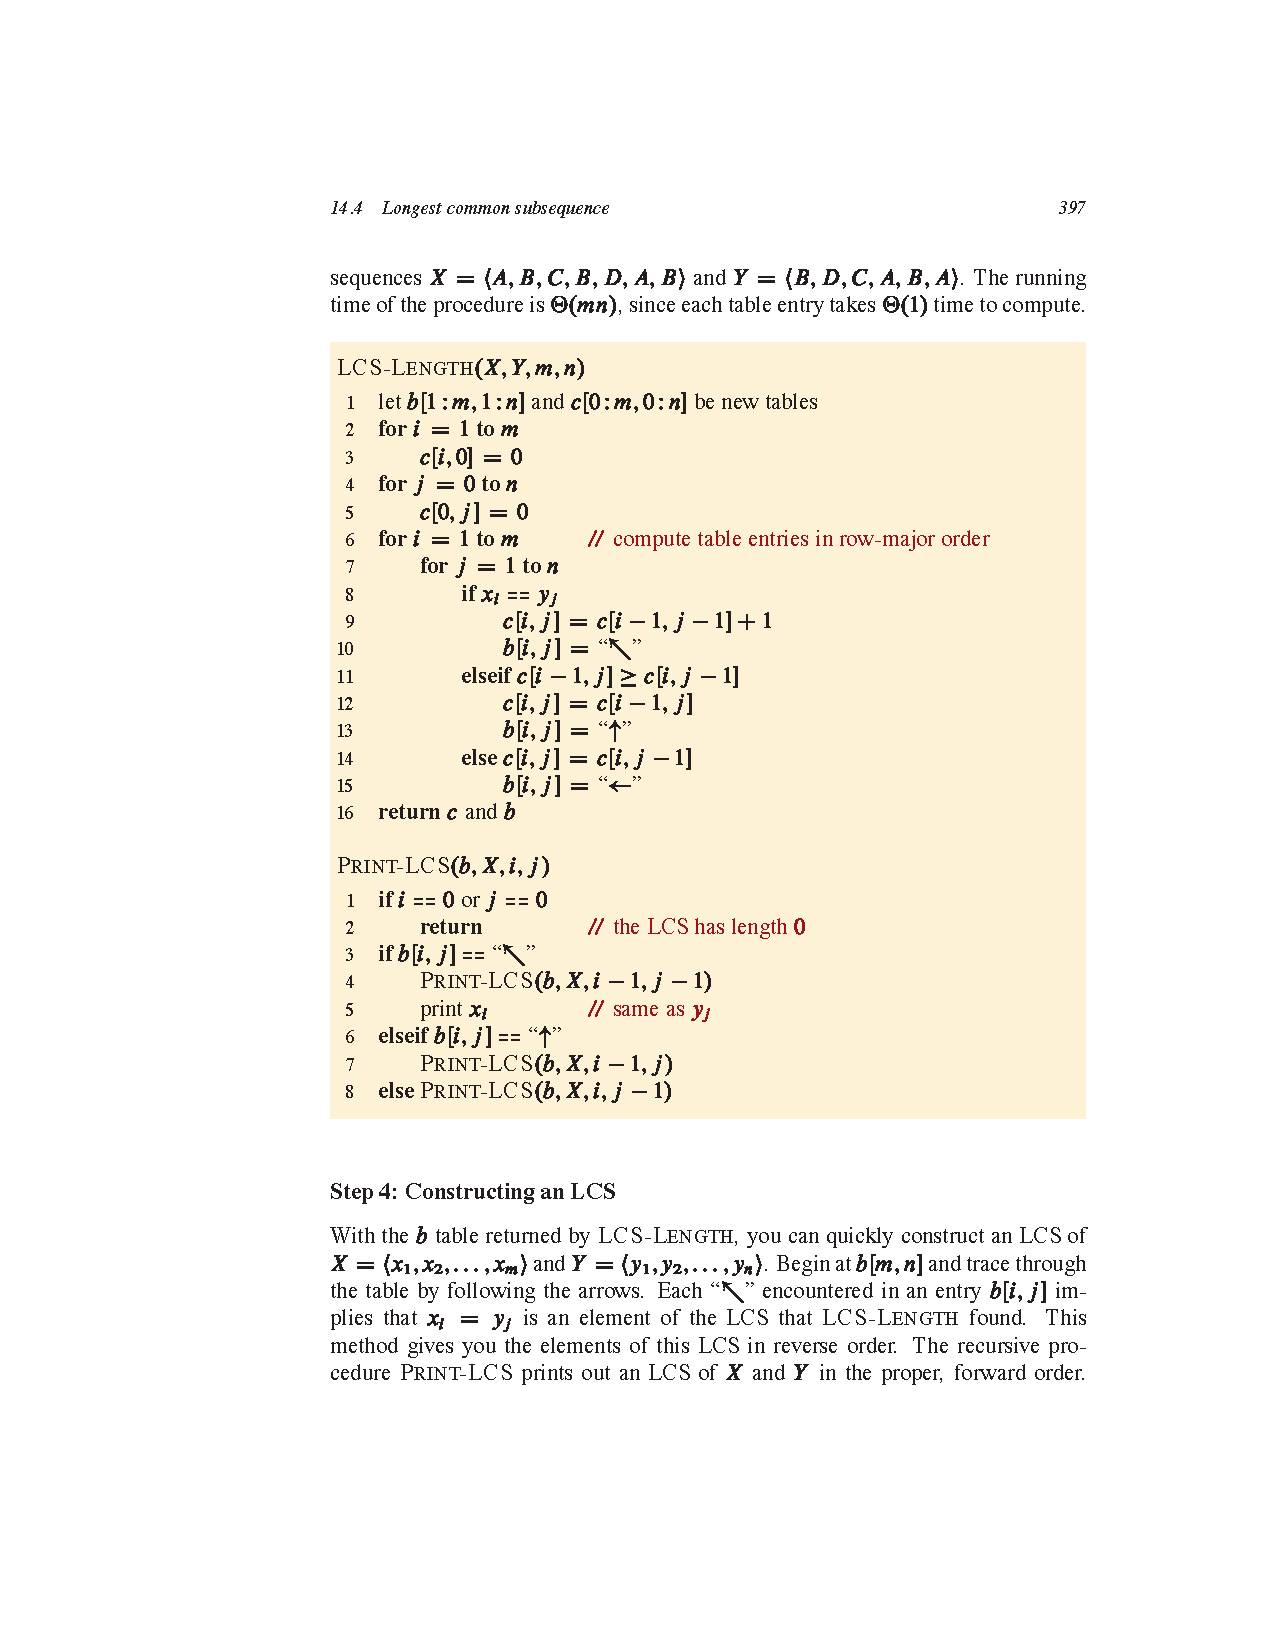
\includegraphics[width=0.7\textwidth,clip,trim=5.50cm 13.75cm 4.5cm 6cm]{figures/pseudocodes}
\end{frame}

\begin{frame}{Longest Common Subsequence -- Formal Steps of DP}{Step 3: Computing the length of an LCS}
    \centering
    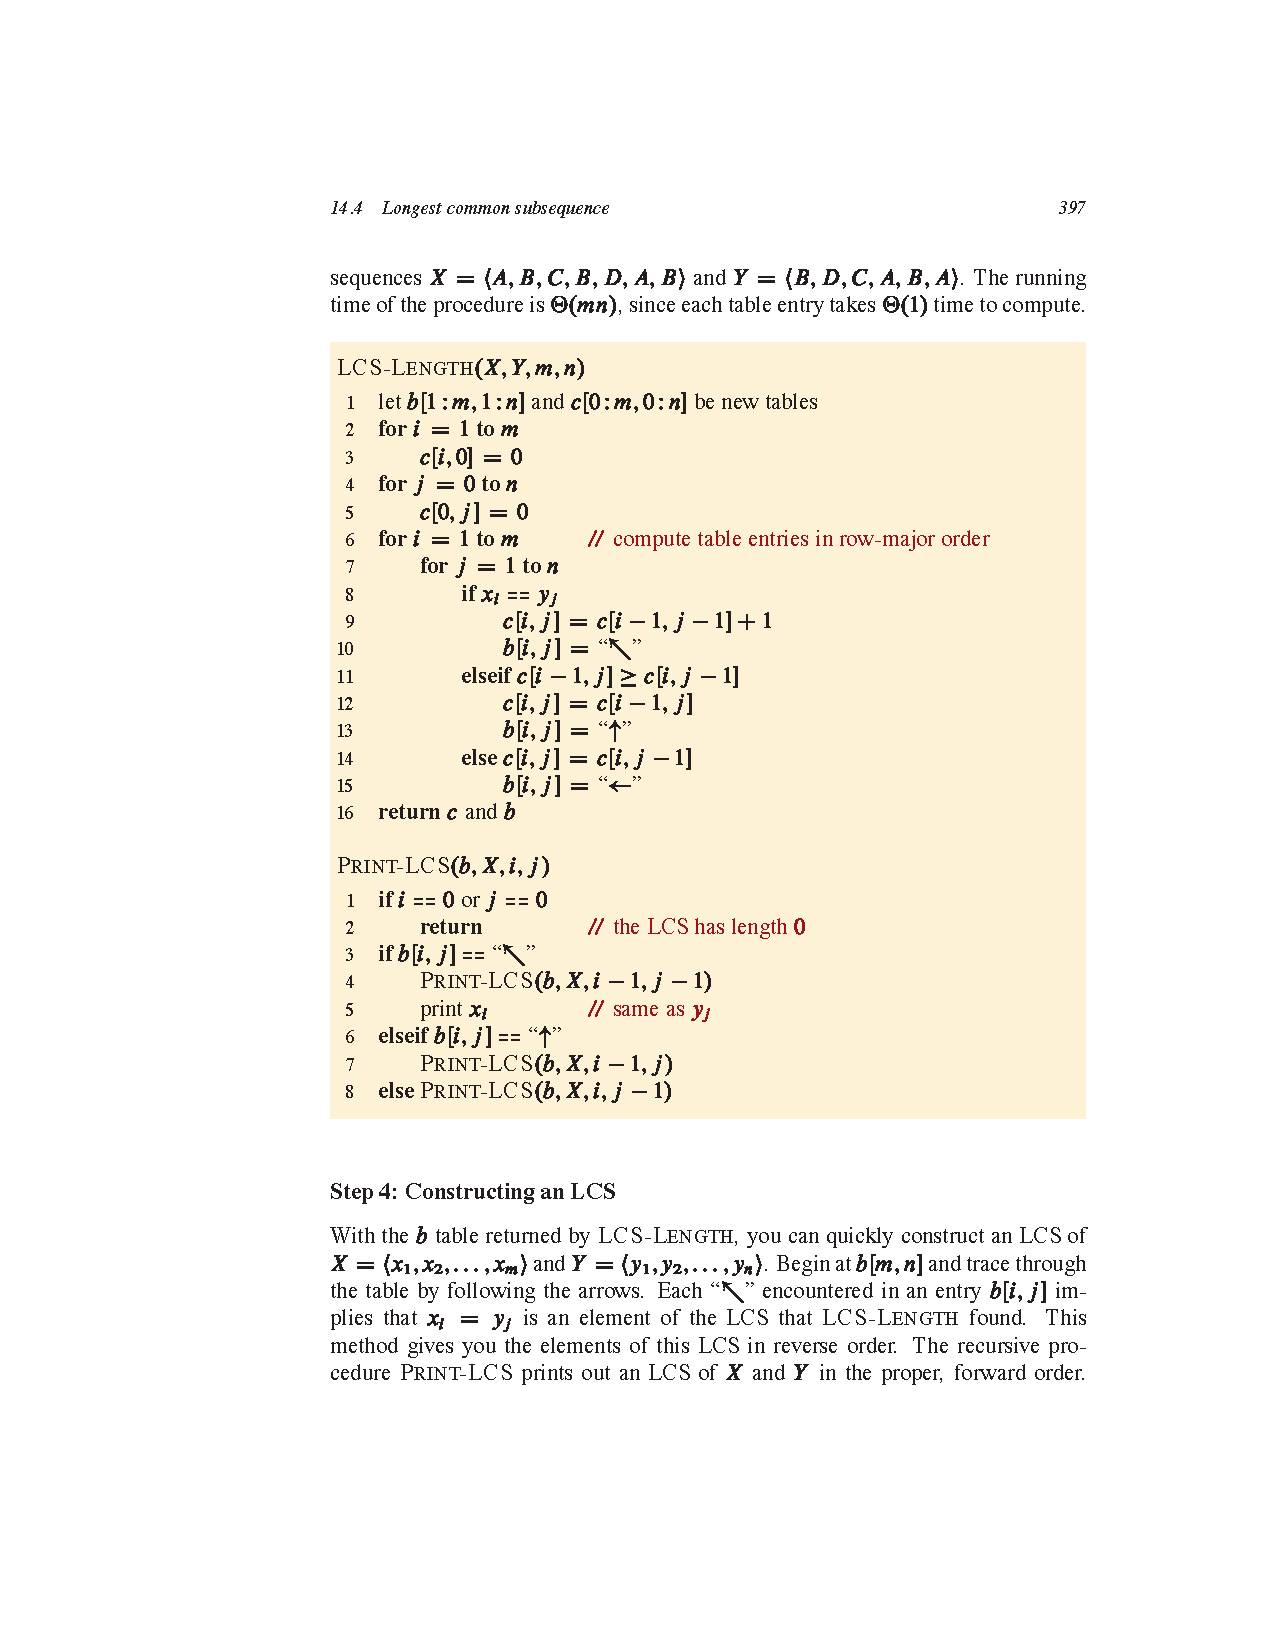
\includegraphics[width=0.7\textwidth,clip,trim=5.50cm 8cm 4.5cm 14.25cm]{figures/pseudocodes}
\end{frame}

\begin{frame}{Longest Common Subsequence -- Formal Steps of DP}{Step 3: Computing the length of an LCS}
    \centering
    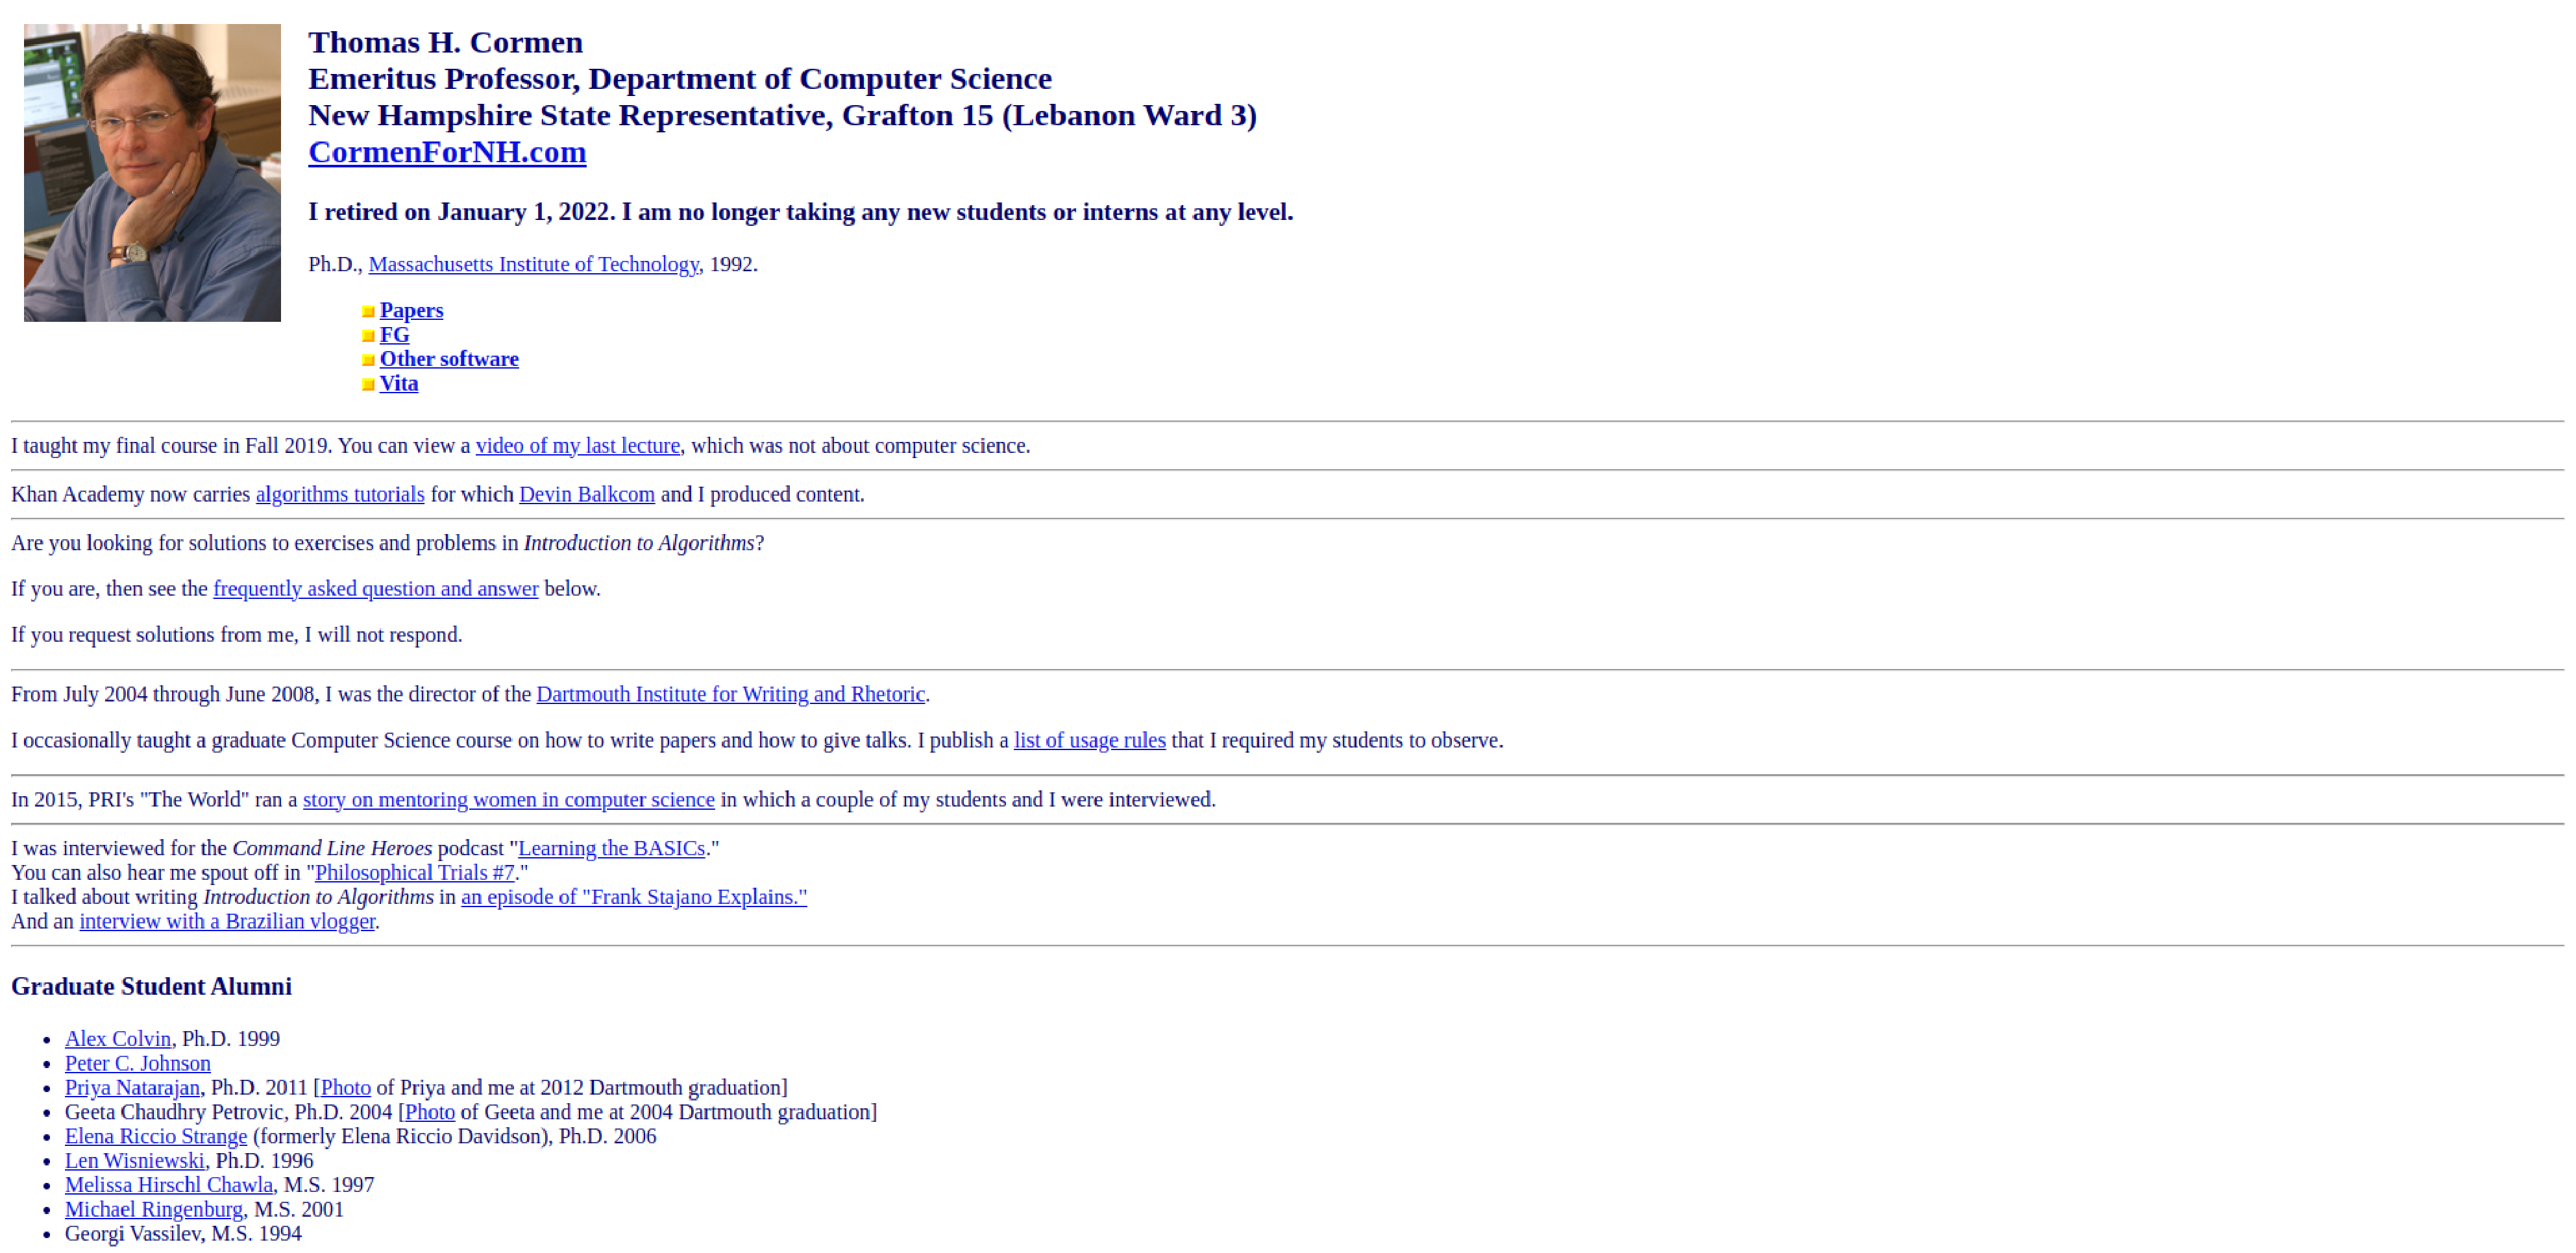
\includegraphics[width=0.9\textwidth]{figures/thc}
    \url{https://www.cs.dartmouth.edu/~thc/} \\
    Implementations \href{https://mitp-content-server.mit.edu/books/content/sectbyfn/books_pres_0/11599/clrsPython.zip}{\textcolor{blue}{\textbf{here}}}
\end{frame}

\begin{frame}{Longest Common Subsequence -- Formal Steps of DP}{Step 3: Computing the length of an LCS}
    \centering
    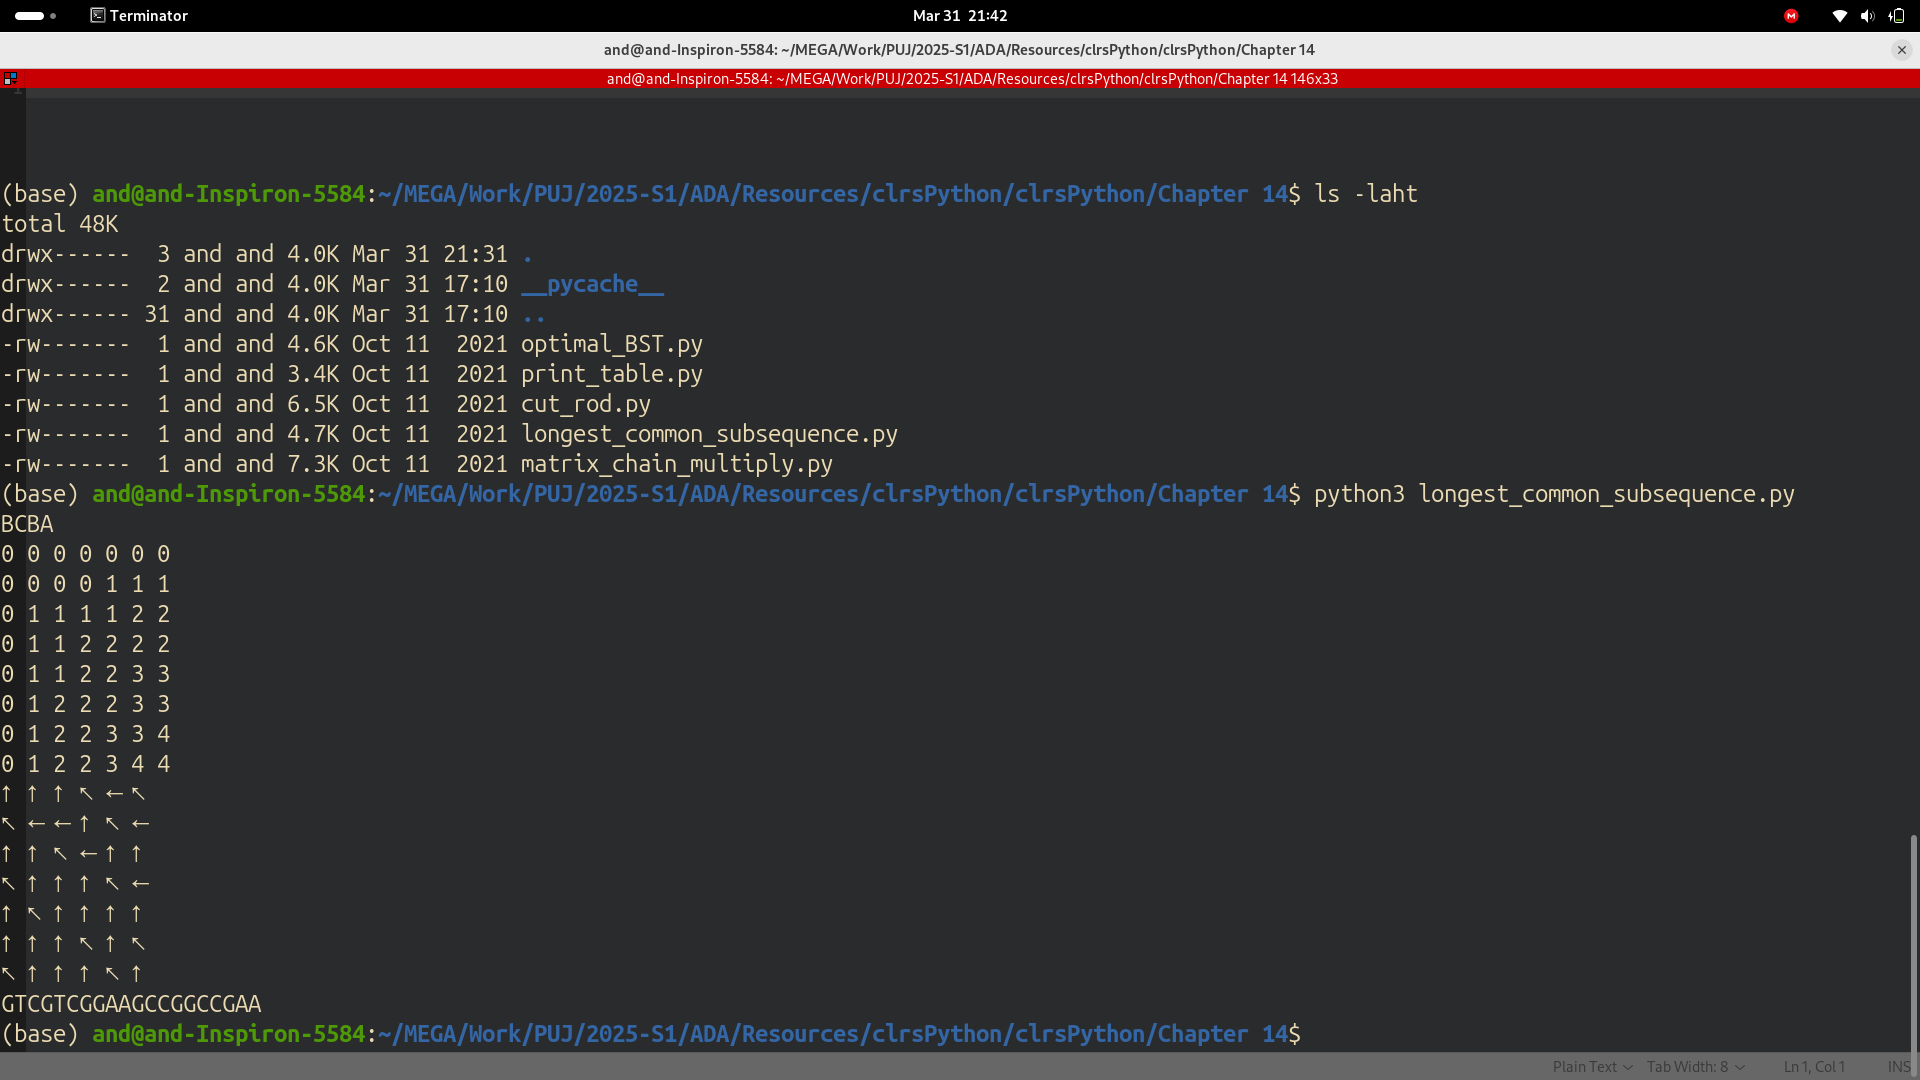
\includegraphics[width=0.9\textwidth]{figures/output}
\end{frame}

\begin{frame}{Longest Common Subsequence -- Formal Steps of DP}{Step 4: Constructing an LCS}
    \centering
    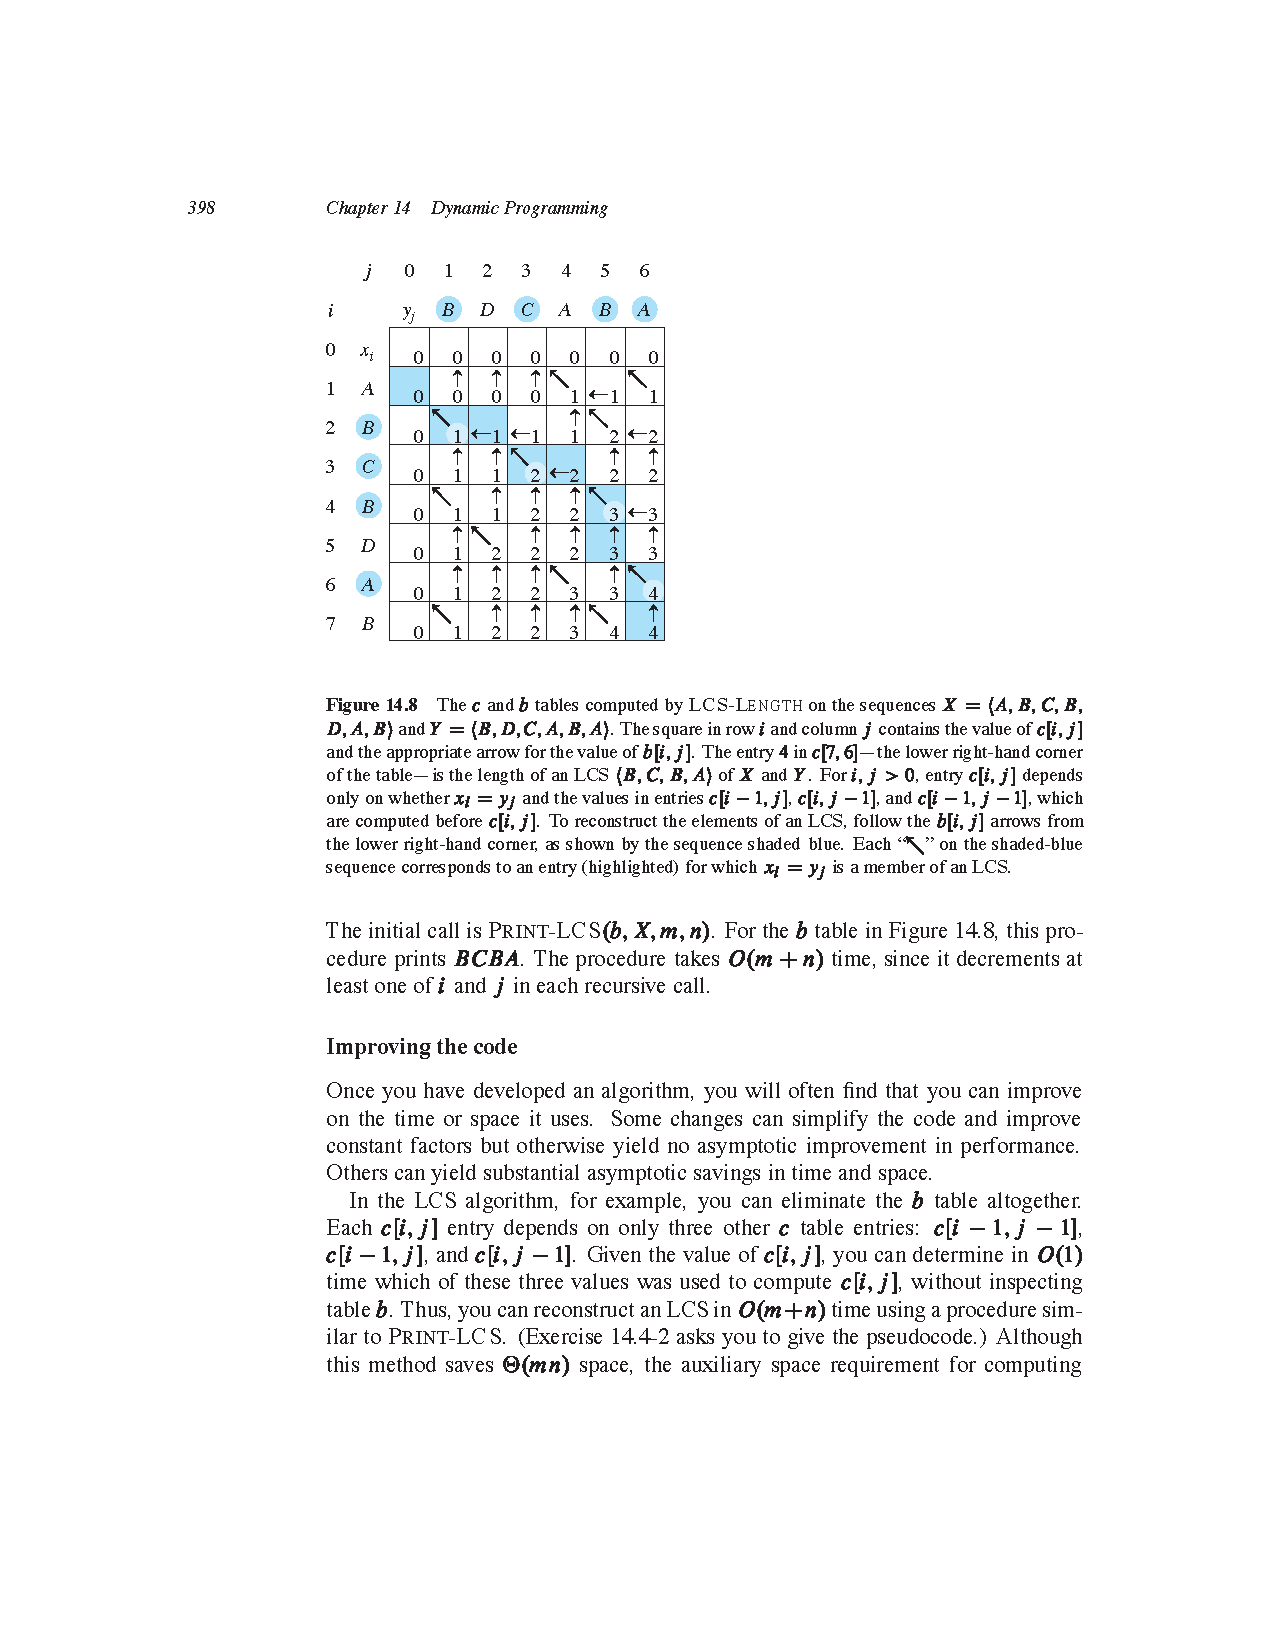
\includegraphics[width=0.62\textwidth,clip,trim=5.53cm 13cm 3.27cm 4cm]{figures/p398}
\end{frame}

\begin{frame}{Homework}
    \Large
    Determine an LCS of $\langle1, 0, 0, 1, 0, 1, 0, 1\rangle$ and $\langle0, 1, 0, 1, 1, 0, 1, 1, 0\rangle$.
\end{frame}

\section{All-pairs shortest paths problem}

\begin{frame}{Introduction}
    Different types of algorithms can be used to solve the all-pairs shortest paths problem:
    \begin{itemize}
        \item Dynamic programming
        \item Matrix multiplication
        \item Floyd-Warshall algorithm
        \item Johnson’s algorithm
        \item Difference constraints
    \end{itemize}
\end{frame}

\begin{frame}{Single-Source Shortest Paths}
    \begin{itemize}
        \item Given directed graph $G = (V, E)$, vertex $s \in V$ and edge weights $w : E \rightarrow \mathbb{R}$
        \item Find $\delta(s, v)$, equal to the shortest-path weight $s \rightarrow v, \forall v \in V$ (or $-\infty$ if negative weight cycle along the way, or $\infty$ if no path)
    \end{itemize} \pause
    \bigskip
    \scriptsize
    \centering
    \begin{tabular}{ c | c | c}
        \textbf{Situtation}         & \textbf{Algorithm}                    & \textbf{Time} \\ \hline
        unweigthed ($w = 1$)        & BFS                                   & \pause $O(V + E)$    \\
        non-negative edge weights   & Dijkstra                              & \pause $O(E + V \lg V)$\\
        general                     & Bellman-Ford                          & \pause $O(VE)$       \\
        acyclic graph (DAG)         & Topological sort + one pass of B-F    & \pause $O(V + E)$    \\
    \end{tabular}\\
    \bigskip
    All of the above results are the best known. We achieve a $O(E + V \lg V )$ bound on Dijkstra’s algorithm using \textbf{Fibonacci heaps}.
\end{frame}

\begin{frame}{All-Pairs Shortest Paths (APSP)}
    \begin{itemize}
        \item Given edge-weighted graph, $G = (V, E, w)$.
        \item Find $\delta(u, v)$ for all $u, v \in V$.
        \item A simple way of solving APSP problems is by running a single-source shortest path algorithm from each of the $V$ vertices in the graph.
    \end{itemize}\pause
    \bigskip
    \tiny
    \centering
    \begin{tabular}{ c | c | c | c}
        \textbf{Situtation}         & \textbf{Algorithm}    & \textbf{Time}         & $E=\Theta(V^2)$ \\ \hline
        unweigthed ($w = 1$)        & $|V| + $ BFS          & $O(V E)$              & $O(V^3)$ \\
        non-negative edge weights   & $|V| + $ Dijkstra     & $O(V E + V^2 \lg V)$  & $O(V^3)$ \\
        general                     & $|V| + $ Bellman-Ford & $O(V^2 E)$            & $O(V^4)$ \\
        general                     & Johnson’s             & $O(V E + V^2 \lg V)$  & $O(V^3)$ \\
    \end{tabular}\\
    \bigskip
    \footnotesize
    These results (apart from the third) are also best known --don’t know how to beat $|V| \times Dijkstra$.
\end{frame}

\begin{frame}{Algorithms to solve APSP}
    Dynamic Programming (attempt 1):
    \begin{enumerate}
    \scriptsize
        \item \textbf{Sub-problems}:
        \item \textbf{Guessing}:
        \item \textbf{Recurrence}:
        \item \textbf{Topological ordering}:
        \item \textbf{Original problem}:
    \end{enumerate}
\end{frame}

\begin{frame}{Algorithms to solve APSP\footnote{\scriptsize For all the algorithms described, we assume that $w(u, v) = \infty$ if $(u, v) \notin E$}}
    Dynamic Programming (attempt 1):
    \begin{enumerate}
    \scriptsize
        \item \textbf{Sub-problems}: $d_{uv}^{(m)} =$ weight of shortest path $u \rightarrow v$ using $\leq m$ edges. \pause
        \item \textbf{Guessing}: What's the last edge (x, v)? \pause
        \item \textbf{Recurrence}:
        \begin{equation*}
            \begin{align*}
                d_{uv}^{(m)} &= min( d_{ux}^{(m - 1)} + w(x, v) & \text{ for } x \in V) \\
                d_{uv}^{(0)} &=
                    \begin{cases}
                        0 & \text{ if } u = v. \\
                        \infty & \text{otherwise}.
                    \end{cases}
            \end{align*}
        \end{equation*} \pause
        \item \textbf{Topological ordering}: for $m = 0, 1, 2, . . . , n - 1$: for $u$ and $v$ in $V$. \pause
        \item \textbf{Original problem}: If graph contains no negative-weight cycles (by Bellman-Ford analysis), then shortest path is simple $\Rightarrow \delta(u, v) = d_{uv}^{(n)} = d_{uv^\prime}^{(n - 1)} = \cdots$
    \end{enumerate}
\end{frame}

\begin{frame}{Bottom-up via Relaxation Steps\footnote{{\scriptsize In the above pseudocode, we omit superscripts because more relaxation can never hurt.}}}
    \begin{codebox}
        \li \For $m \gets 1$ \To $n$ \By 1
        \li \hspace{0.5cm} \For u in V
        \li \hspace{1.0cm} \For v in V
        \li \hspace{1.5cm} \For x in V
        \li \hspace{2.0cm} \If $d_{uv} > d_{ux} + d_{xv}$
        \li \hspace{2.5cm} $d_{uv} = d_{ux} + d_{xv}$
    \end{codebox}
\end{frame}

\begin{frame}{Time complexity}
    \begin{itemize}
        \item In this Dynamic Program, we have $O(V^3)$ total sub-problems.
        \item Each sub-problem takes $O(V)$ time to solve, since we need to consider $V$ possible choices.
        \item This gives a total runtime complexity of $O(V^4)$.
        \item Note that this is no better than $|V| \times$ Bellman-Ford.
    \end{itemize}
\end{frame}

\begin{frame}{Matrix Multiplication}
    Recall the task of standard matrix multiplication:
    \begin{itemize}
        \item Given $n \times n$ matrices $A$ and $B$, compute $C = A \cdot B$, such that $c_{ij} = \sum_{k=1}^{n} a_{ik} \cdot b_{kj}$. \pause
        \begin{enumerate}
            \item $O(n^3)$ using standard algorithm. \pause
            \item $O(n^{2.807})$  using Strassen algorithm. \pause
            \item $O(n^{2.376})$  using Coppersmith-Winograd algorithm. \pause
            \item $O(n^{2.3728})$ using Vassilevska-Williams algorithm.
        \end{enumerate}
    \end{itemize}
\end{frame}

\begin{frame}{Connection to Shortest Paths}
    \begin{itemize}
        \item Let's define $\oplus = \min$ and $\odot = +$.
        \item Then, $C = A \odot B$ produces $c_{ij} = \min_k (a_{ik} + b_{kj})$.
        \item Define $D^{(m)} = (d_{ij}^{(m)})$, $W = (w(i, j))$, $V = \{1,2, \ldots, n\}$
    \end{itemize}
    \bigskip
    With the above definitions, we see that $D^{(m)}$ can be expressed as $D^{(m-1)} \odot W$. In other words, $D^{(m)}$ can be expressed as the circle-multiplication of $W$ with itself $m$ times.
\end{frame}

\begin{frame}{Matrix Multiplication Algorithm}
    \begin{itemize}
        % $n - 2$ multiplications
        \item $\Rightarrow O(n^4)$ time (still no better). \pause
        \item Repeated squaring: $((W^2)^2)^{2 \cdots}$ \pause $= W^{2^{\lg n}}$ \pause $= W^{n - 1} = (\delta(i, j))$ if no negative-weight cycles. \pause
        \item Time complexity of this algorithm is now \textcolor{red}{$O(n^3 \lg n)$}.
    \end{itemize}
\end{frame}

\begin{frame}{Floyd-Warshall Algorithms}
    Dynamic Programming (attempt 2):
    \begin{enumerate}
        \item \textbf{Sub-problems}: $c_{uv}^{(k)} =$ weight of shortest path $u \rightarrow v$ whose intermediate vertices $\in \{1,2, \ldots, k\}$ \pause
        \item \textbf{Guessing}:  \pause Does shortest path use vertex $k$? \pause
        \item \textbf{Recurrence}:
        \begin{equation*}
            \begin{align*}
                c_{uv}^{(0)} &= w(u, v) \\
                c_{uv}^{(k)} &= \min(c_{uv}^{(k-1)}, c_{ux}^{(k-1)} + c_{xv}^{(k-1)})
            \end{align*}
        \end{equation*}  \pause
        \item \textbf{Topological order}: for $k$: for $u$ and $v$ in $V$:
        \item \textbf{Original problem}: $\delta(u, v) = c_{uv}^{(n)}$. Negative weight cycle $\Leftrightarrow$ negative $c_{uu}^{(n)}$
    \end{enumerate}
\end{frame}

\begin{frame}{Time Complexity}
    This Dynamic Program contains $O(V^3)$ problems as well. However, in this case, it takes only $O(1)$ time to solve each sub-problem, which means that the total runtime of this algorithm is $O(V^3)$.
\end{frame}

\begin{frame}{Bottom-up via Relaxation}
    \begin{codebox}
        \li $C = (w(u, v))$
        \li \For $k \gets 1$ \To $n$
        \li \hspace{0.5cm} \For u in V
        \li \hspace{1.0cm} \For v in V
        \li \hspace{1.5cm} \If $c_{uv} > c_{uk} + c_{kv}$
        \li \hspace{2.0cm} $c_{uv} = c_{uk} + c_{kv}$
    \end{codebox}
\end{frame}

\begin{frame}{Johnson’s algorithm}
    \begin{enumerate}
        \item Find function $h: V \rightarrow \mathbb{R}$ such that $w_h (u, v) = w(u, v) + h(u) - h(v) \geq 0$ for all $u, v \in V$ or determine that a negative-weight cycle exists.
        \item Run Dijkstra’s algorithm on $(V, E, w_h)$ from every source vertex $s \in V \Rightarrow$ get $\delta_h (u, v)$ for all $u, v \in V$.
        \item Given $\delta_h (u, v)$, it is easy to compute $\delta(u, v)$.
    \end{enumerate}
\end{frame}

\begin{frame}{Proof}
    \textbf{Claim}. $\delta(u, v) = \delta_h (u, v) - h(u) + h(v)$. \\
    \\
    \textit{Proof}. Look at any $u \rightarrow v$ path $p$ in the graph $G$:
    \begin{itemize}
        \footnotesize
        \item Say $p$ is $v_0 \rightarrow v_1 \rightarrow v_2 \rightarrow \cdots \rightarrow v_k$, where $v_0 = u$ and $v_k = v$.
        \begin{equation*}
            \begin{align*}
                w_h (p) &= \sum_{i = 1}^{k} w_h (v_{i - 1}, v_i) \\
                        &= \sum_{i = 1}^{k} [w(v_{i - 1}, v_i) + h(v_{i-1}) - h(v_i)] \\
                        &= \sum_{i = 1}^{k} w(v_{i - 1}, v_i) + h(v_0) - h(v_k) \\
                        &= w(p) + h(u) - h(v)
            \end{align*}
        \end{equation*}
        \item Hence all $u \rightarrow v$ paths change in weight by the same offset $h(u) - h(v)$, which implies that the shortest path is preserved. \qed
    \end{itemize}
\end{frame}

\begin{frame}{How to find $h$?}
    We know that
        $$w_h (u, v) = w(u, v) + h(u) - h(v) \geq 0$$
    This is equivalent to,
        $$h(v) - h(u) \leq w(u, v)$$
    for all $(u, v) \in V$. This is called a \textbf{system of difference constraints}.
    \begin{tcolorbox}[title=Theorem.]
        If $(V, E, w)$ has a negative-weight cycle, then there exists no solution to the above system of difference constraints.
    \end{tcolorbox}
\end{frame}

\begin{frame}{\textit{Proof}}
    \scriptsize
    Say $v_0 \rightarrow v_1 \rightarrow \cdots \rightarrow v_k \rightarrow v_0$ is a negative weight cycle.\\
    Let us assume to the contrary that the system of difference constraints has a solution; let's call it $h$.\\
    This gives us the following system of equations,

    \begin{equation*}
        \begin{align*}
            h(v_1) - h(v_0) & \leq w(v_0, v_1) \\
            h(v_2) - h(v_1) & \leq w(v_1, v_2) \\
            h(v_3) - h(v_2) & \leq w(v_2, v_3) \\
                            & \vdots \\
            h(v_k) - h(v_{k-1}) & \leq w(v_{k-1}, v_k) \\
            h(v_0) - h(v_k) & \leq w(v_k, v_0) \\
        \end{align*}
    \end{equation*}

    Summing all these equations gives us
    $$
        0 \leq w(cycle) < 0
    $$
    which is obviously not possible. \\
    From this, we can conclude that no solution to the above system of difference constraints exists if the graph $(V, E, w)$ has a negative weight cycle. \qed
\end{frame}

\begin{frame}{}
    \begin{tcolorbox}[title=Theorem.]
        If $(V, E, w)$ has no negative-weight cycle, then we can find a solution to the difference constraints.
    \end{tcolorbox}
    \scriptsize
    \textit{Proof}. Add a new vertex $s$ to $G$, and add edges $(s, v)$ of weight $0$ for all $v \in V$.
    \begin{itemize}
        \item Clearly, these new edges do not introduce any new negative weight cycles to the graph.
        \item Adding these new edges ensures that there now exists at least one path from $s$ to $v$. This implies that $\delta(s, v)$ is finite for all $v \in V$
        \item We now claim that $h(v) = \delta(s, v)$. This is obvious from the triangle inequality: $\delta(s, u) + w(u, v) \geq \delta(s, v) \Leftrightarrow \delta(s, v) - \delta(s, u) \leq w(u, v) \Leftrightarrow h(v) - h(u) \leq w(u, v)$. \qed
    \end{itemize}
\end{frame}

\begin{frame}{Time Complexity}
    \begin{enumerate}
        \item The first step involves running Bellman-Ford from $s$, which takes $O(VE)$ time.  We also pay a pre-processing cost to reweight all the edges ($O(E)$). \pause
        \item We then run Dijkstra's algorithm from each of the $V$ vertices in the graph; the total time complexity of this step is $O(VE + V^2 \lg V)$. \pause
        \item We then need to reweight the shortest paths for each pair; this takes $O(V^2)$ time. \pause
    \end{enumerate}
    The total running time of this algorithm is \textcolor{red}{$O(VE + V^2 \lg V)$}.
\end{frame}

\section{Rod Cutting Problem}

\begin{frame}{Rod Cutting Problem}
    \textbf{Problem Statement:}\\
    Given a rod of length $n$ inches and a table of prices $p_i$ for $i = 1, 2, \dots, n$, determine the maximum revenue obtainable by cutting the rod and selling the pieces.

    \vspace{1em}
    \textbf{Example Price Table:}
    \centering
    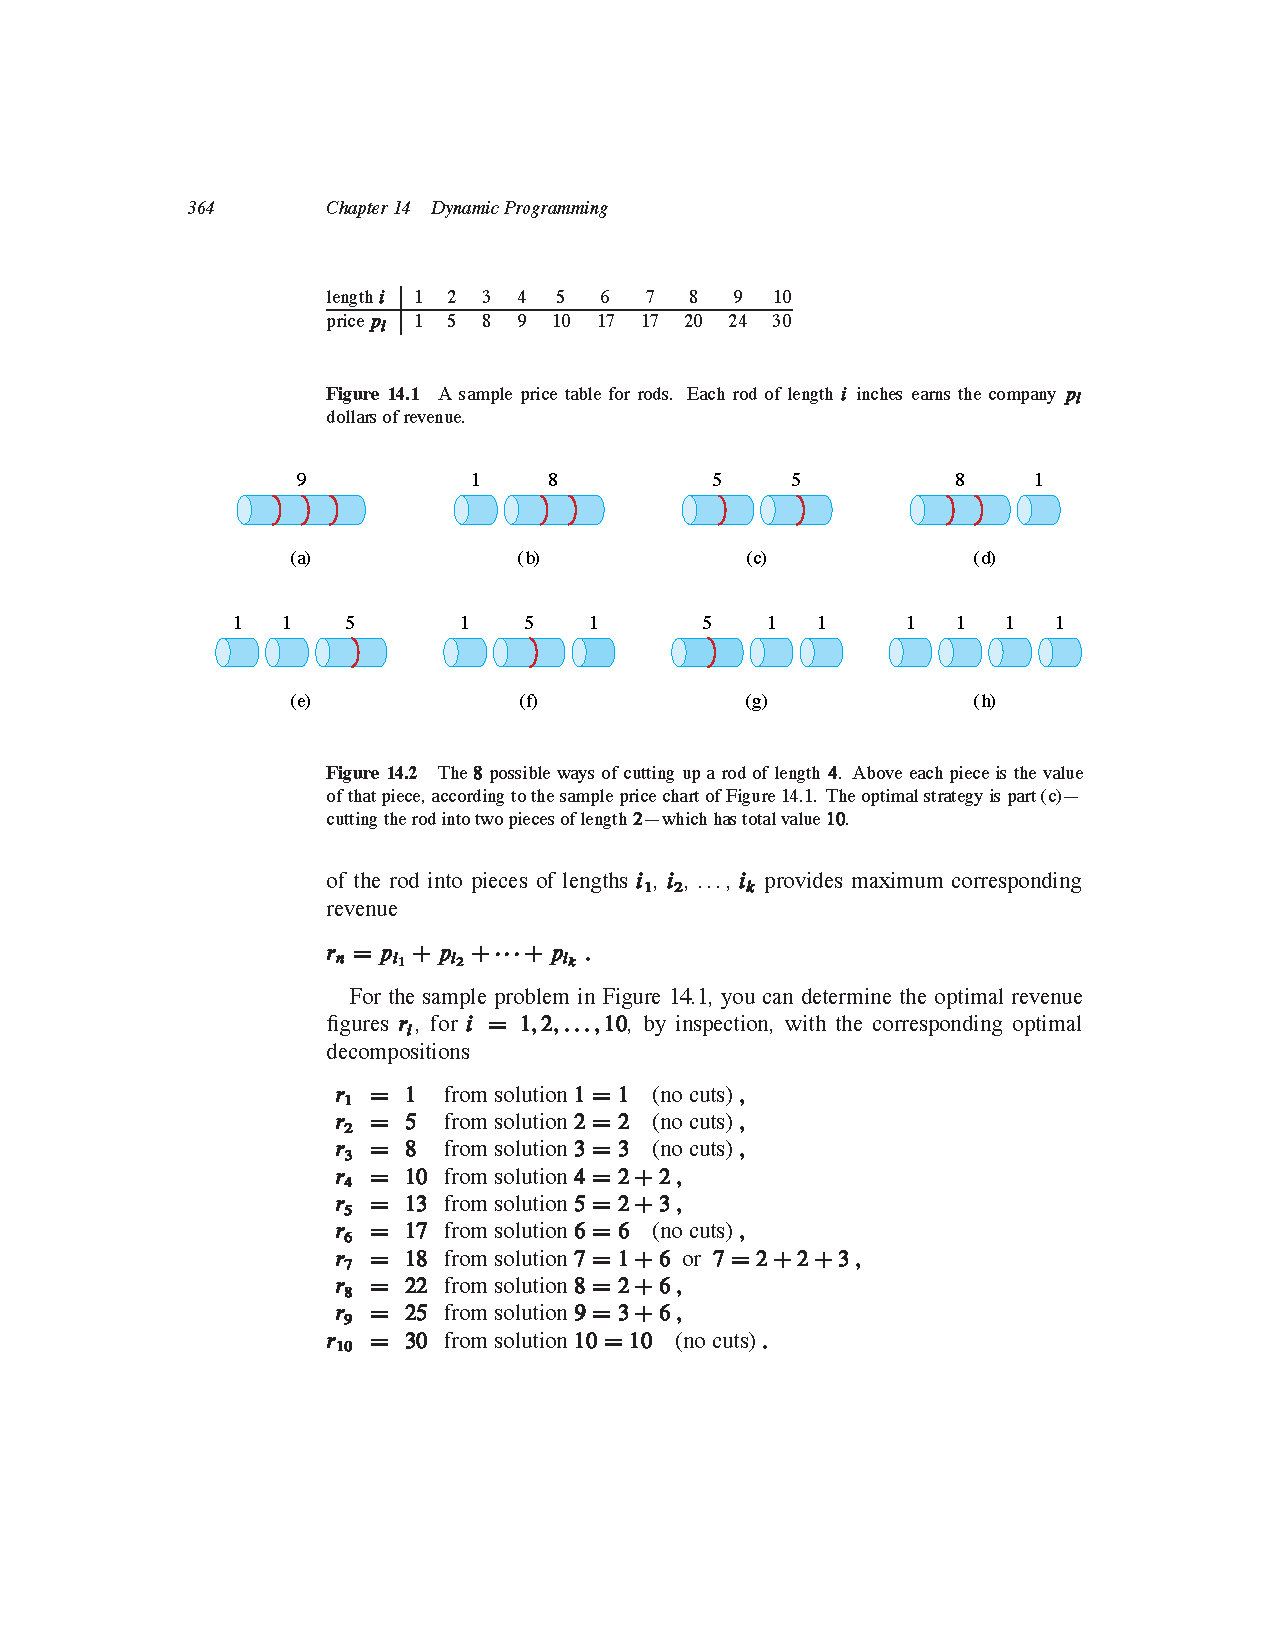
\includegraphics[width=\textwidth,clip=true,trim=5cm 22cm 8cm 4.5cm]{figures/p364}
\end{frame}

\begin{frame}{Problem Statement}
    \centering
    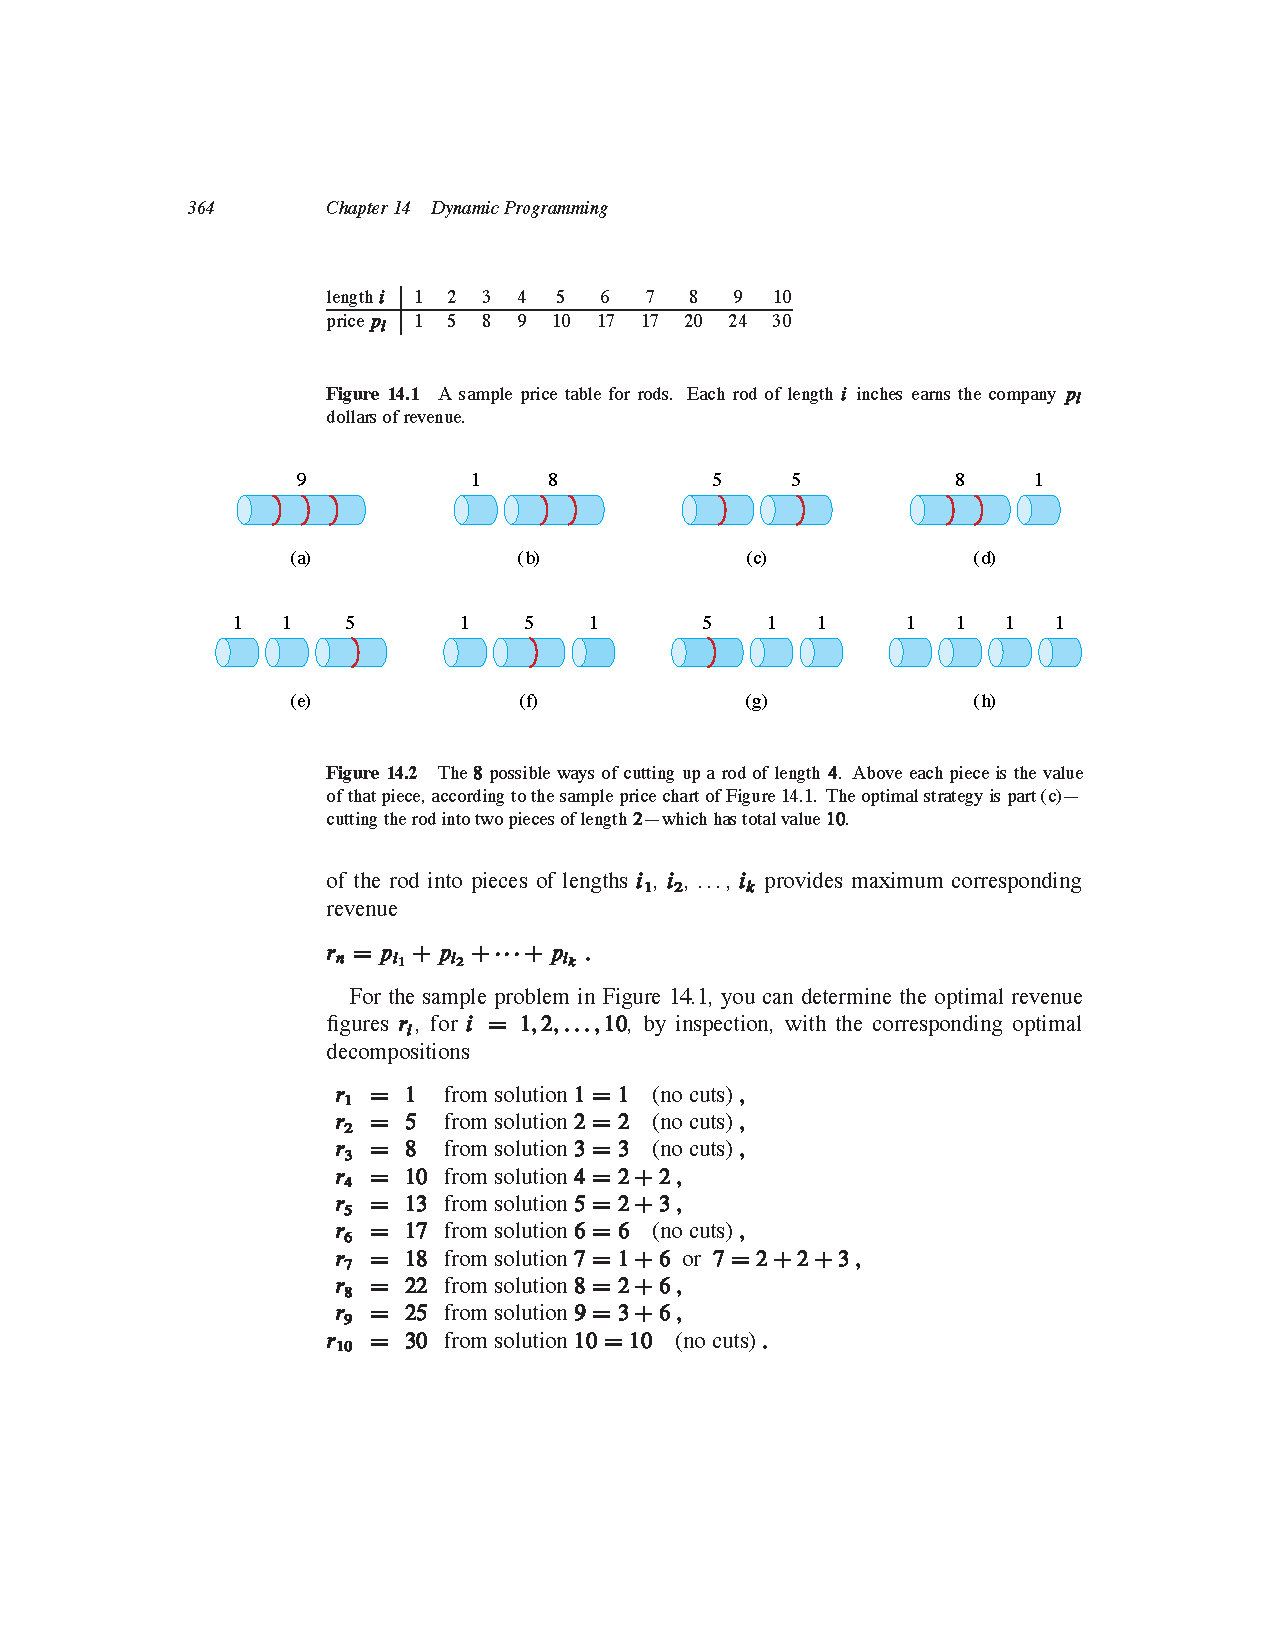
\includegraphics[width=\textwidth,clip=true,trim=3cm 13.5cm 3cm 8cm]{figures/p364}
\end{frame}

\begin{frame}{Recursive Formulation}
    Let $r_n$ be the maximum revenue for a rod of length $n$. Then:

    \[
        r_n = \max_{1 \leq i \leq n} (p_i + r_{n-i})
    \]
    \textbf{Base case:} $r_0 = 0$ \\

    \vspace{1em}
    \textbf{Exponential Time Algorithm:}
    \centering
    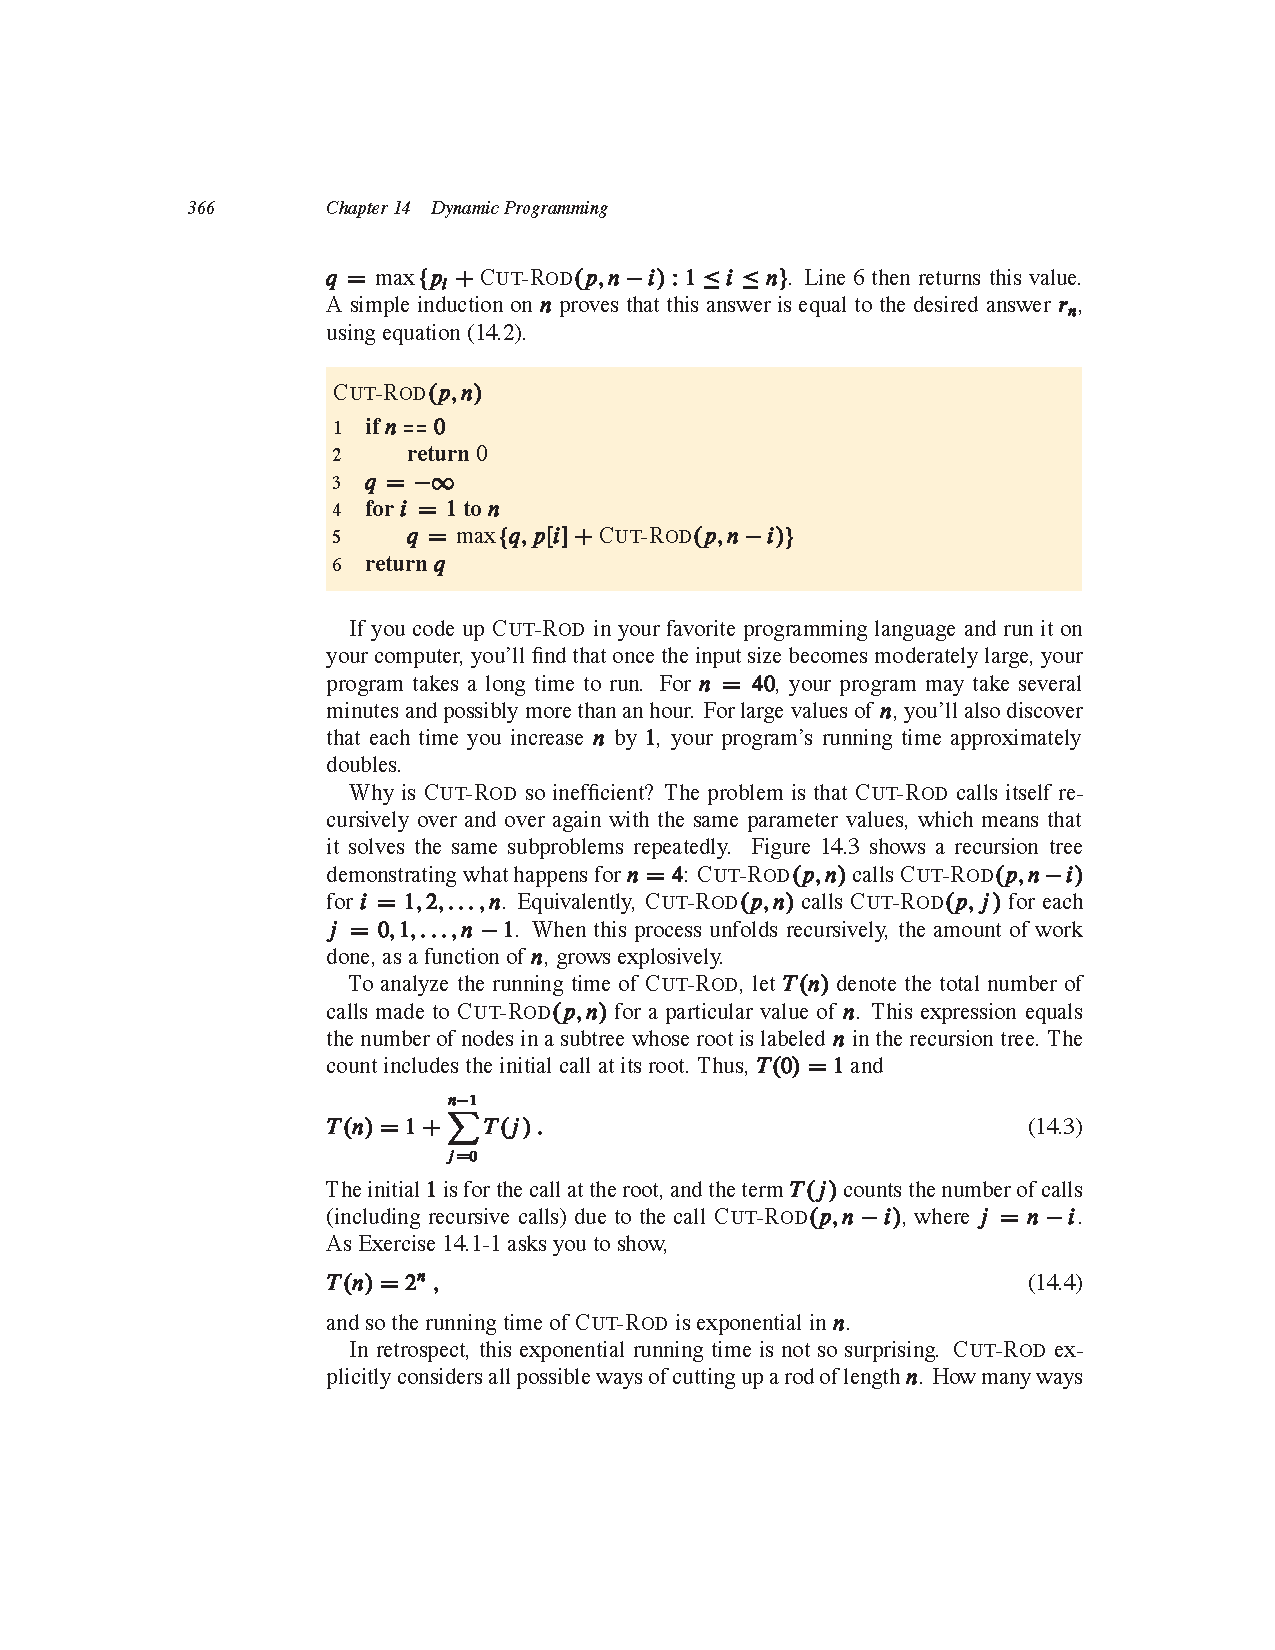
\includegraphics[width=\textwidth,clip=true,trim=4.75cm 18cm 3cm 6cm]{figures/p366}
\end{frame}

\begin{frame}{Recursive Formulation}
    \begin{itemize}
        \item Let $T(n)$ denote the total number of calls made to \textsc{cut-rod}$(p,n)$ for a particular value of $n$.
        \item The number of nodes in a subtree whose root is labeled $n$ in the recursion tree.
    \end{itemize}
    $$
        T(n) = 1 + \sum_{j = 0}^{n - 1} T(j).
    $$
\end{frame}

\begin{frame}{Recursive Formulation}
    \centering
    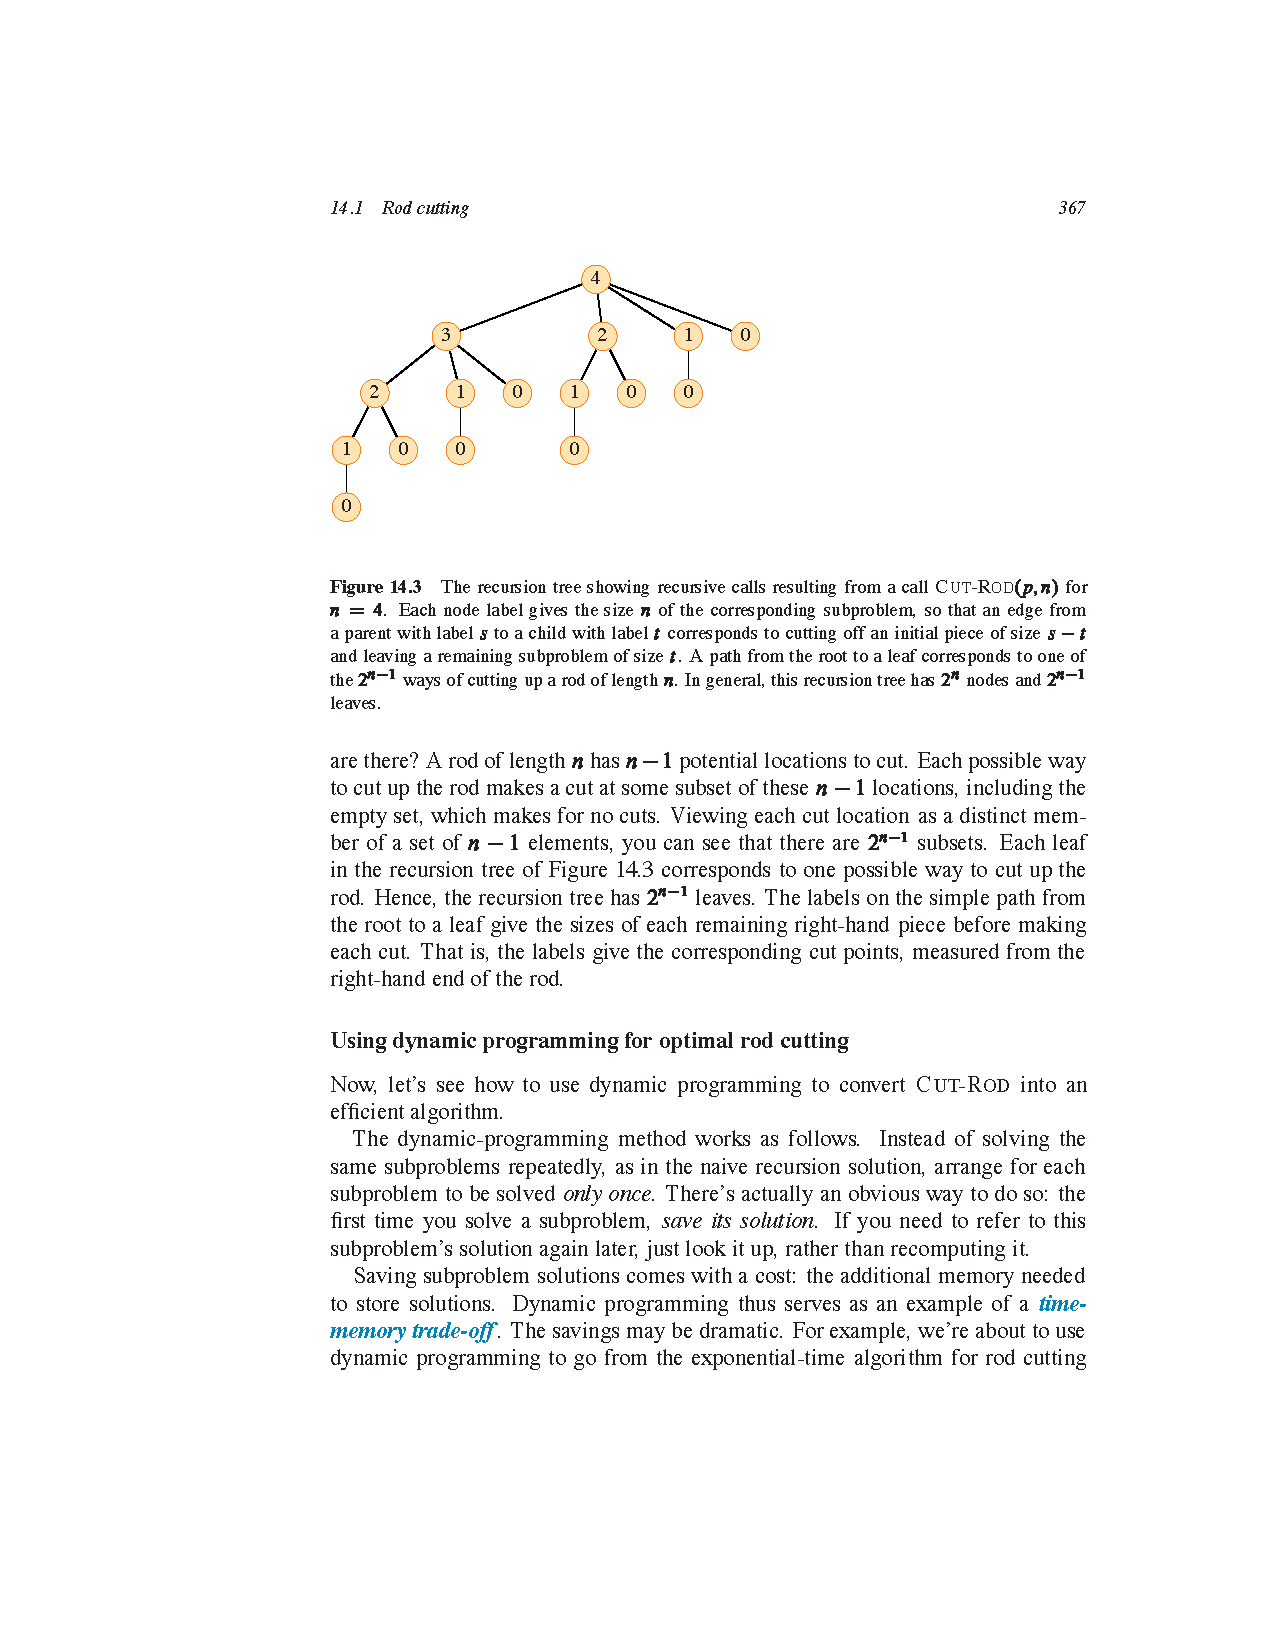
\includegraphics[width=0.95\textwidth,clip=true,trim=5cm 19cm 8cm 4cm]{figures/p367}
\end{frame}

\begin{frame}{Memoized Version}
    Avoids recomputation by storing already computed values.

    \centering
    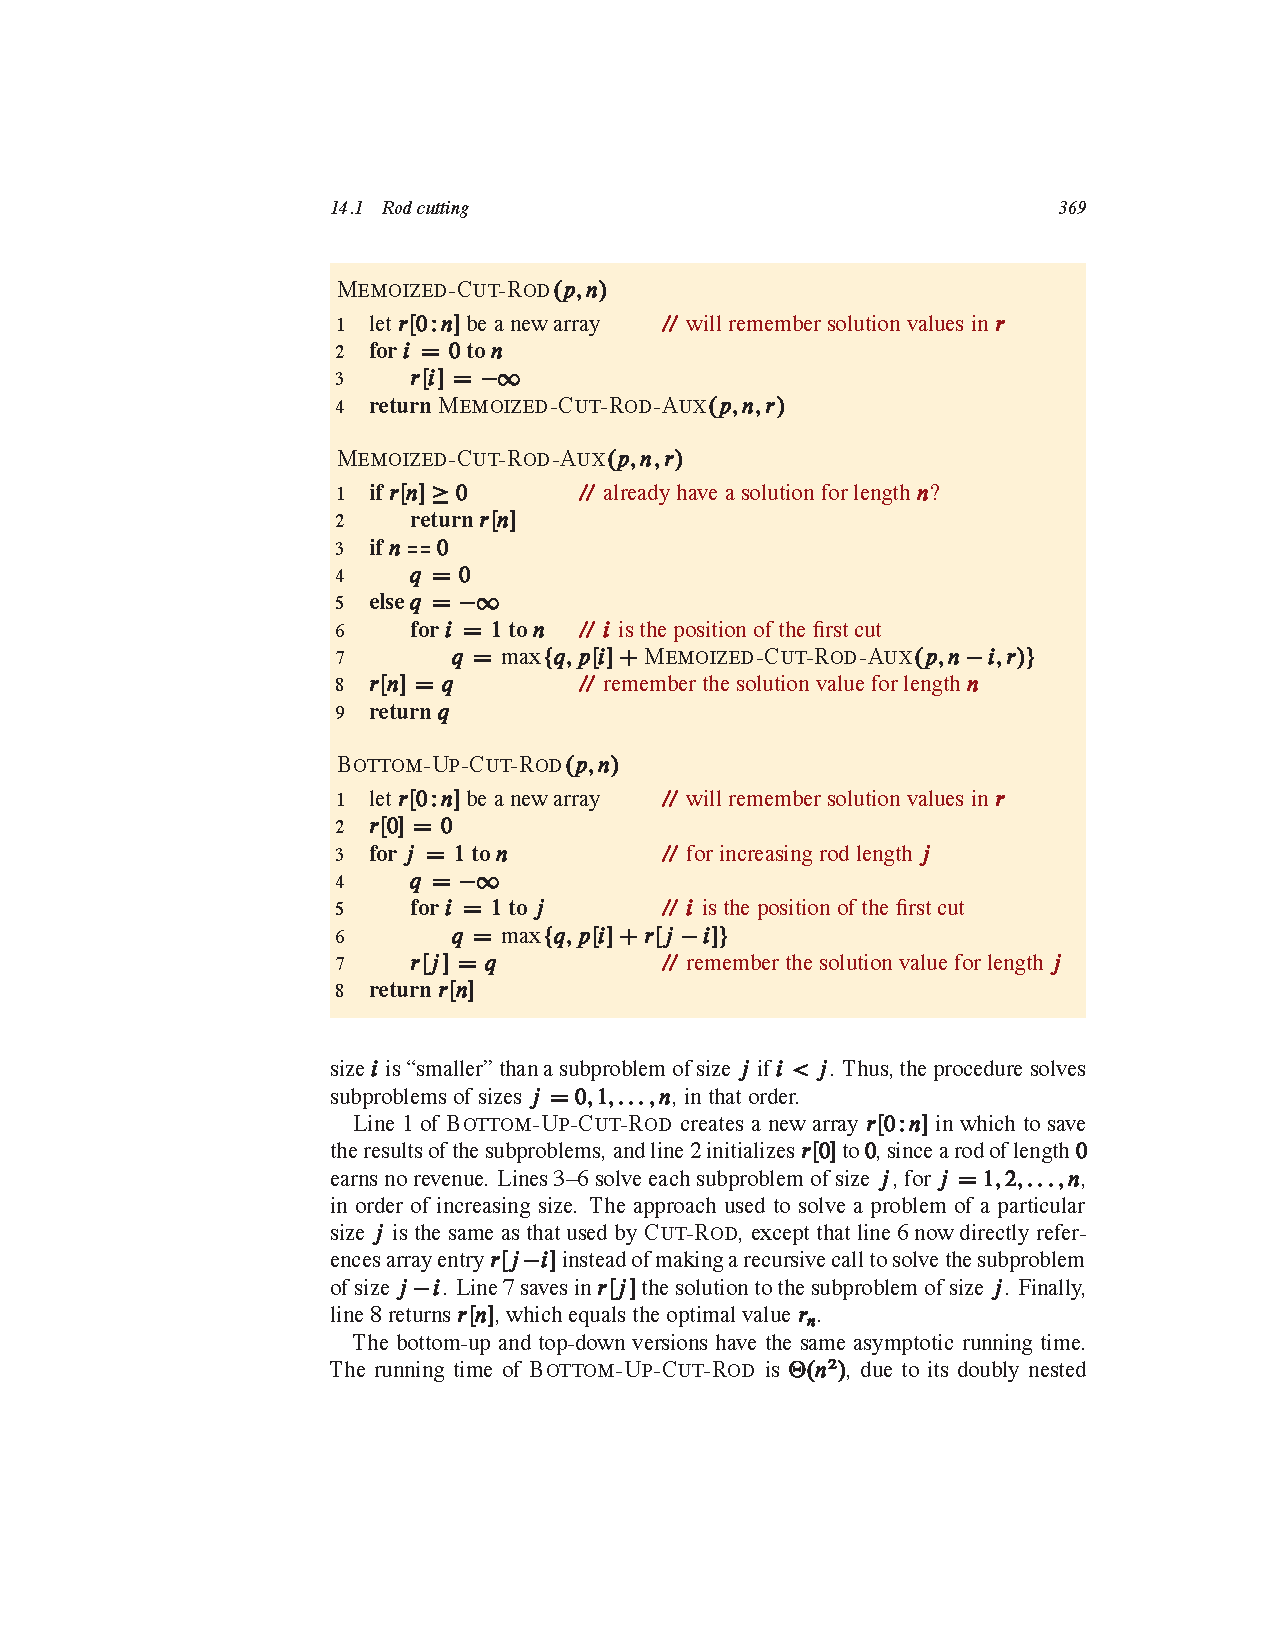
\includegraphics[width=0.8\textwidth,clip=true,trim=5cm 15.5cm 3cm 4cm]{figures/p369}
\end{frame}

\begin{frame}{Bottom-Up Dynamic Programming}
    \centering
    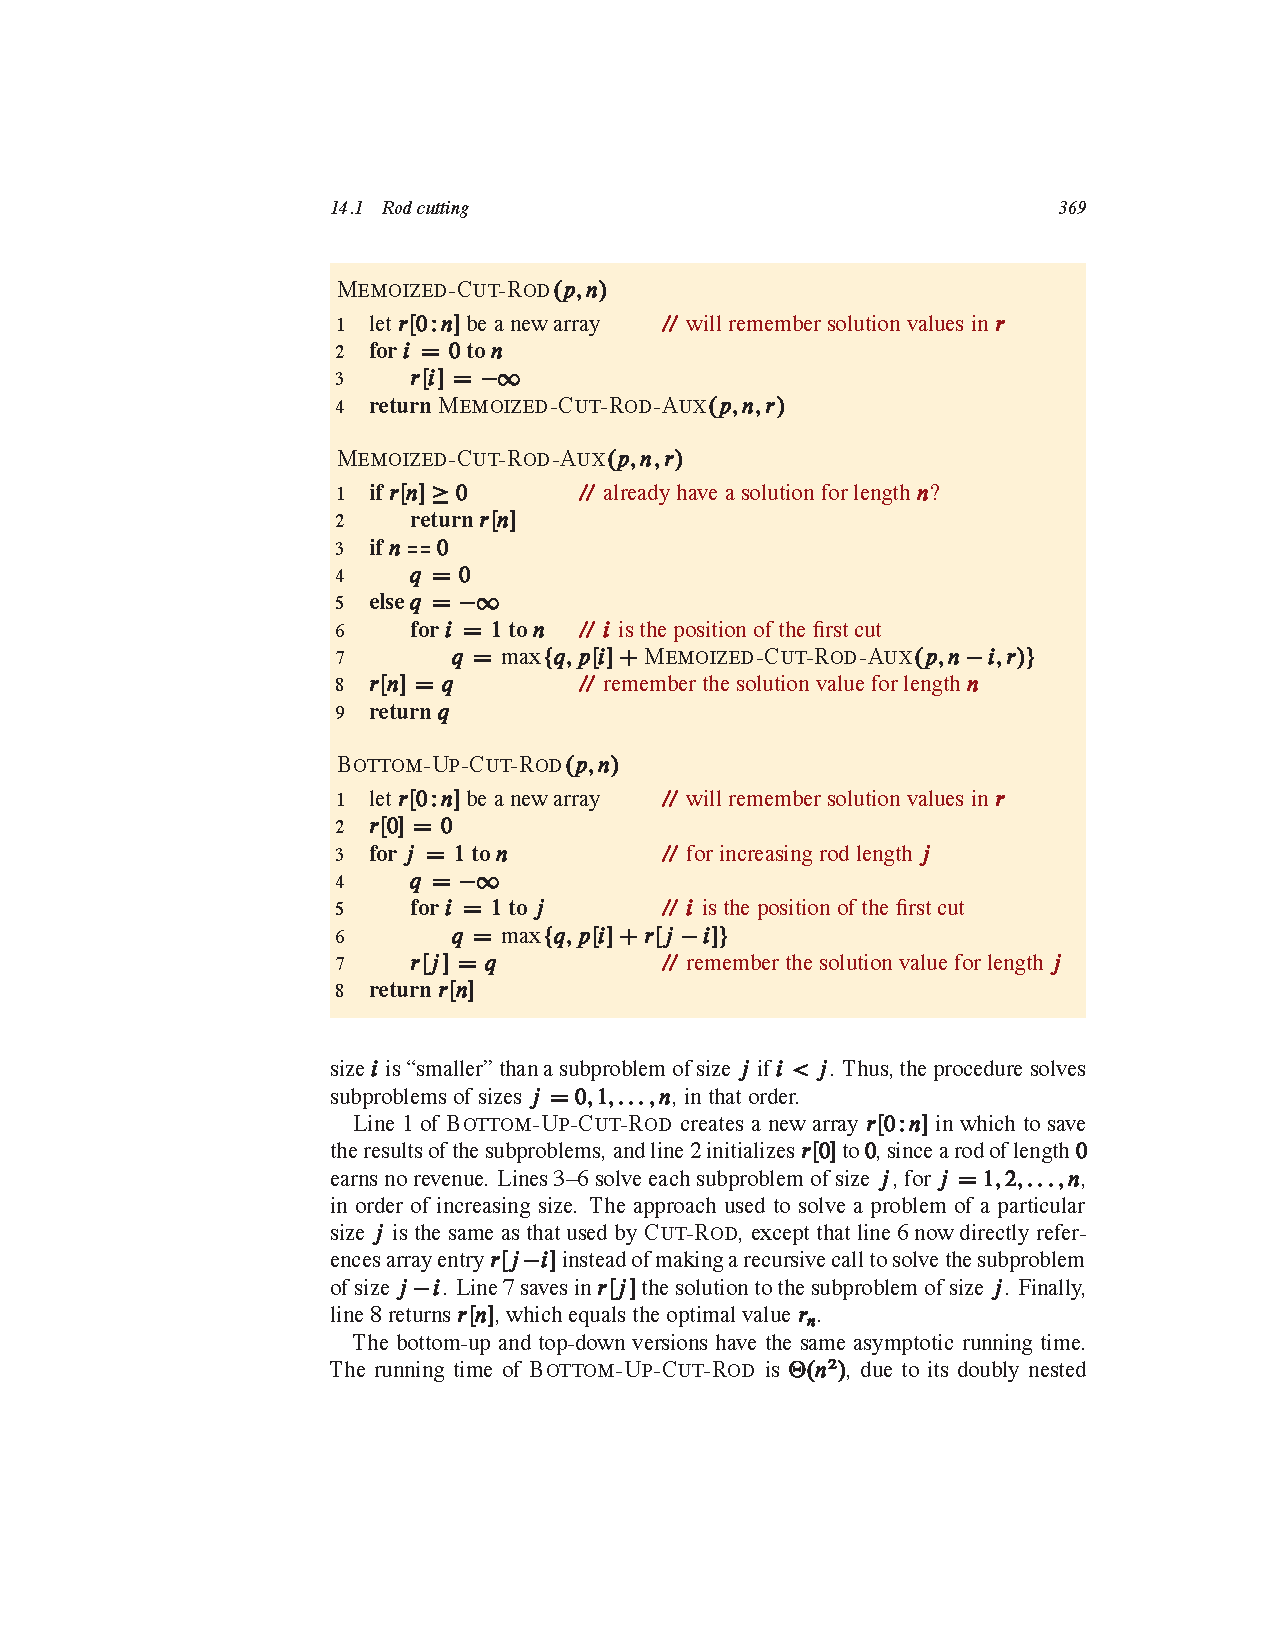
\includegraphics[width=\textwidth,clip=true,trim=5cm 10.5cm 3cm 12.5cm]{figures/p369}

    \textbf{Time complexity:} $\mathcal{O}(n^2)$
\end{frame}

\begin{frame}{Subproblem graphs}
    \centering
    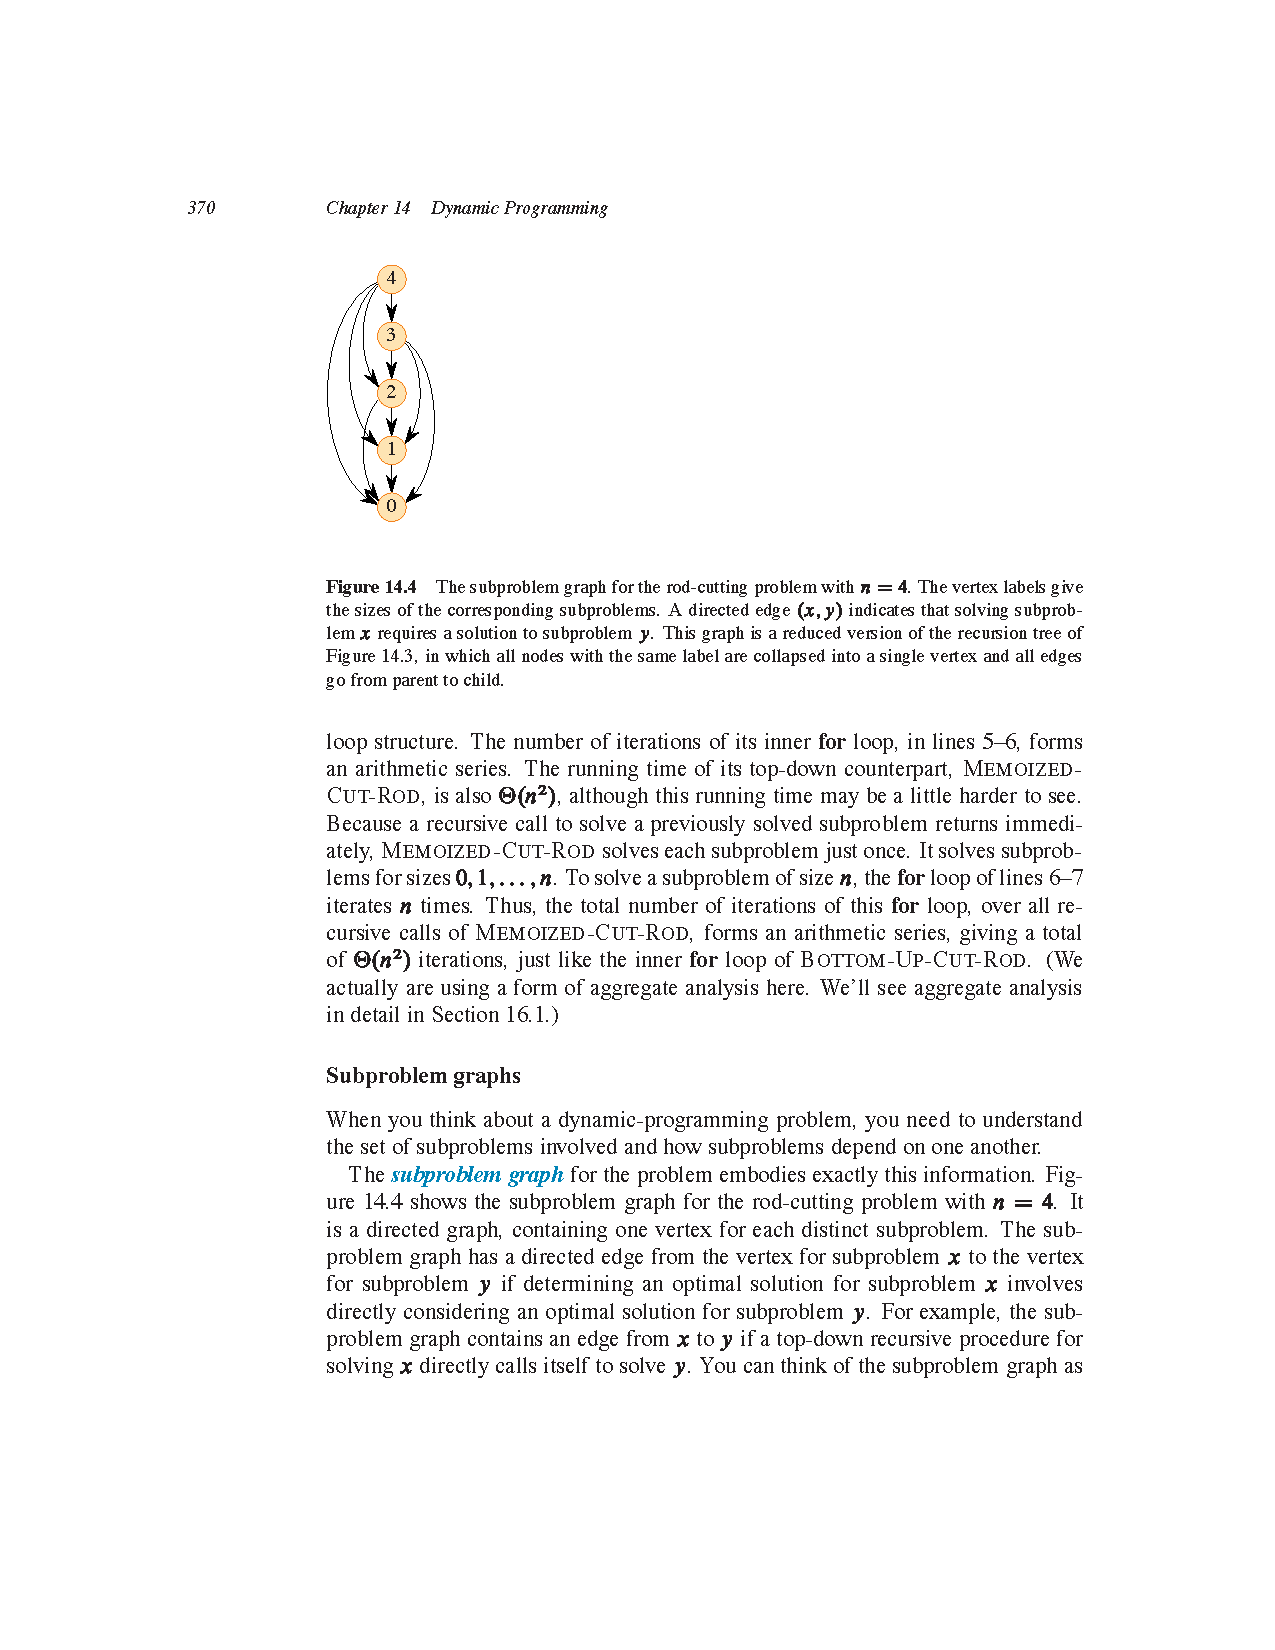
\includegraphics[width=0.9\textwidth,clip=true,trim=5cm 16cm 3cm 4cm]{figures/p370}
\end{frame}

\begin{frame}{Reconstructing the Solution}
    Store the optimal cuts as well:

    \begin{itemize}
        \item Maintain a second array $s[1..n]$.
        \item $s[j]$ stores the length of the first piece to cut from a rod of length $j$.
    \end{itemize}

    Then backtrack using $s[n]$ to print the actual cuts.\\
    \vspace{5mm}
    \begin{tabular}{c | r r r r r r r r r r r }
        \large
        $i$ & 0 & 1 & 2 & 3 & 4 & 5 & 6 & 7 & 8 & 9 & 10 \\ \hline
        $r[i]$ & 0 & 1 & 5 & 8 & 10 & 13 & 17 & 18 & 22 & 25 & 30 \\
        $s[i]$ &   & 1 & 2 & 3 & 2 & 2 & 6 & 1 & 2 & 3 & 10 \\
    \end{tabular}
\end{frame}

\begin{frame}{Reconstructing a solution}
    \centering
    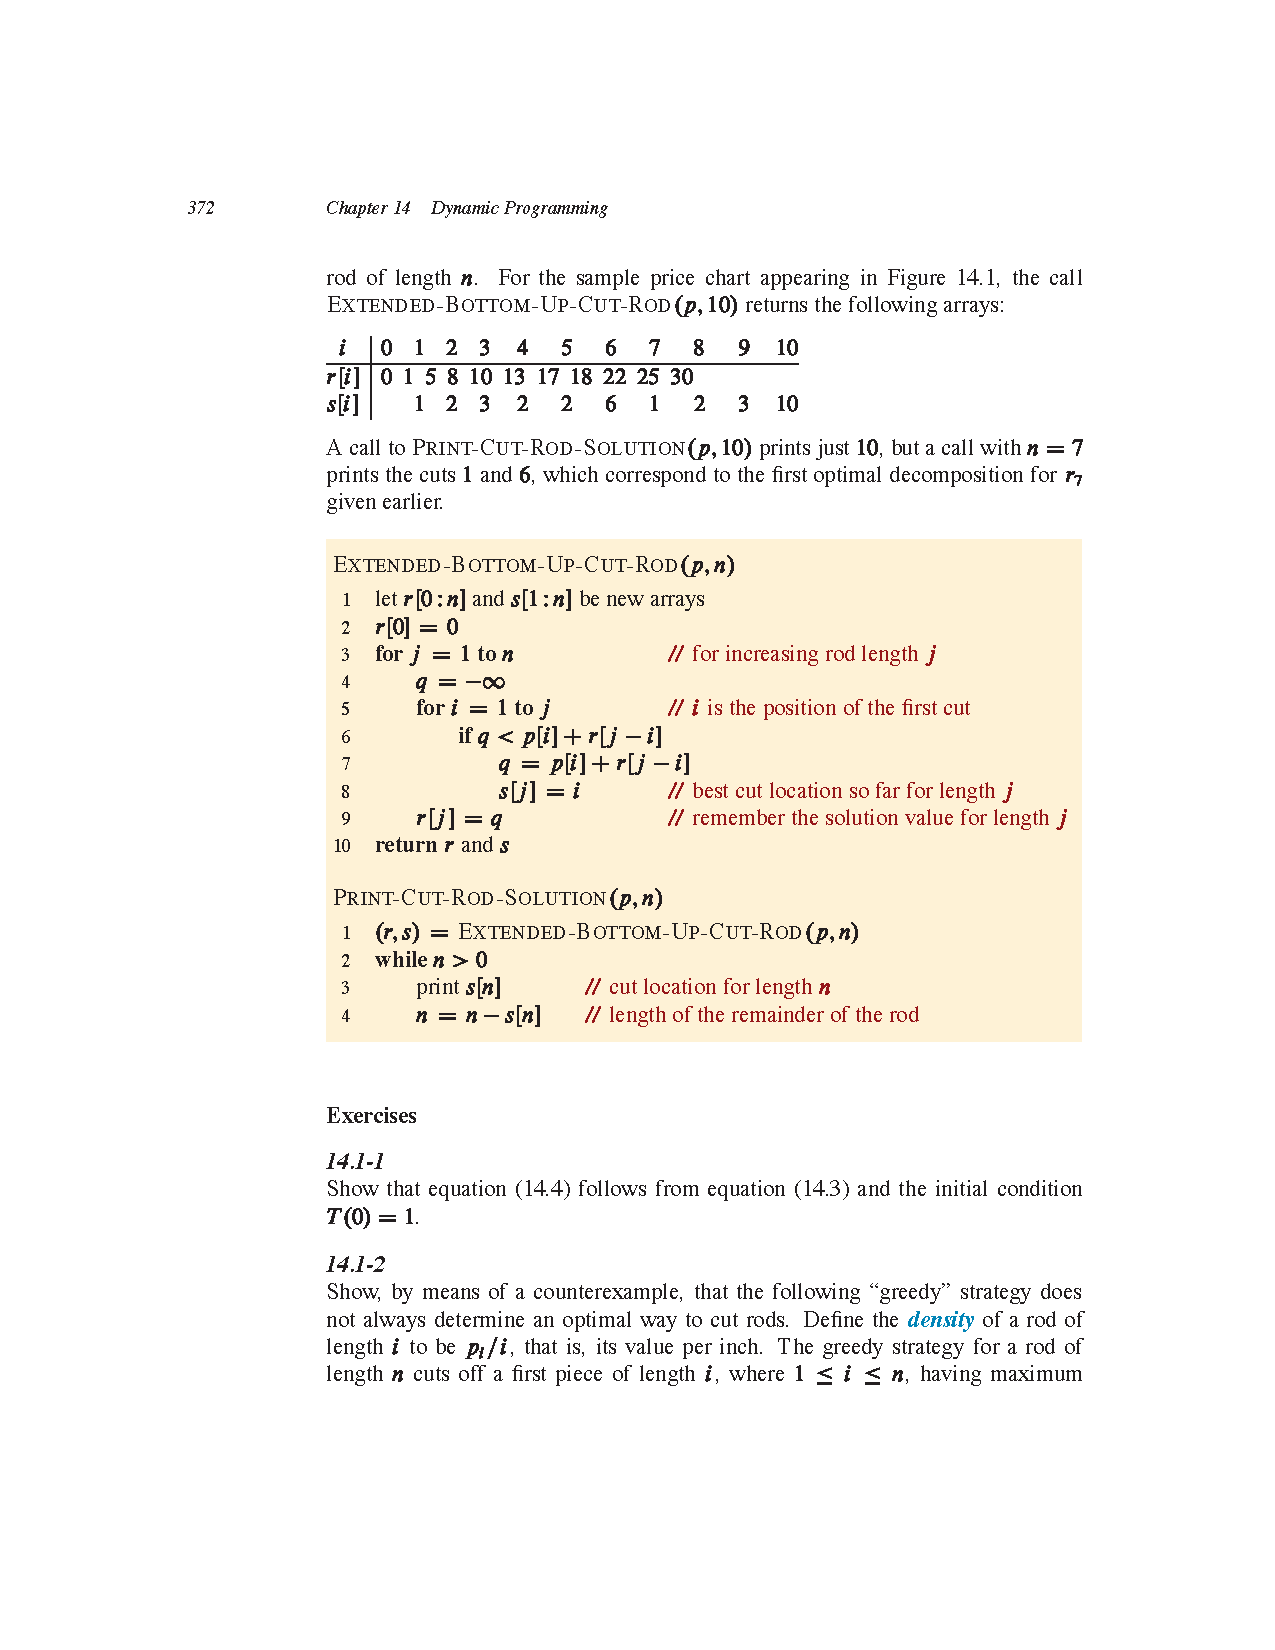
\includegraphics[width=\textwidth,clip=true,trim=5cm 13cm 3cm 9cm]{figures/p372}
\end{frame}

\begin{frame}{Code Implemantation}
    \centering
    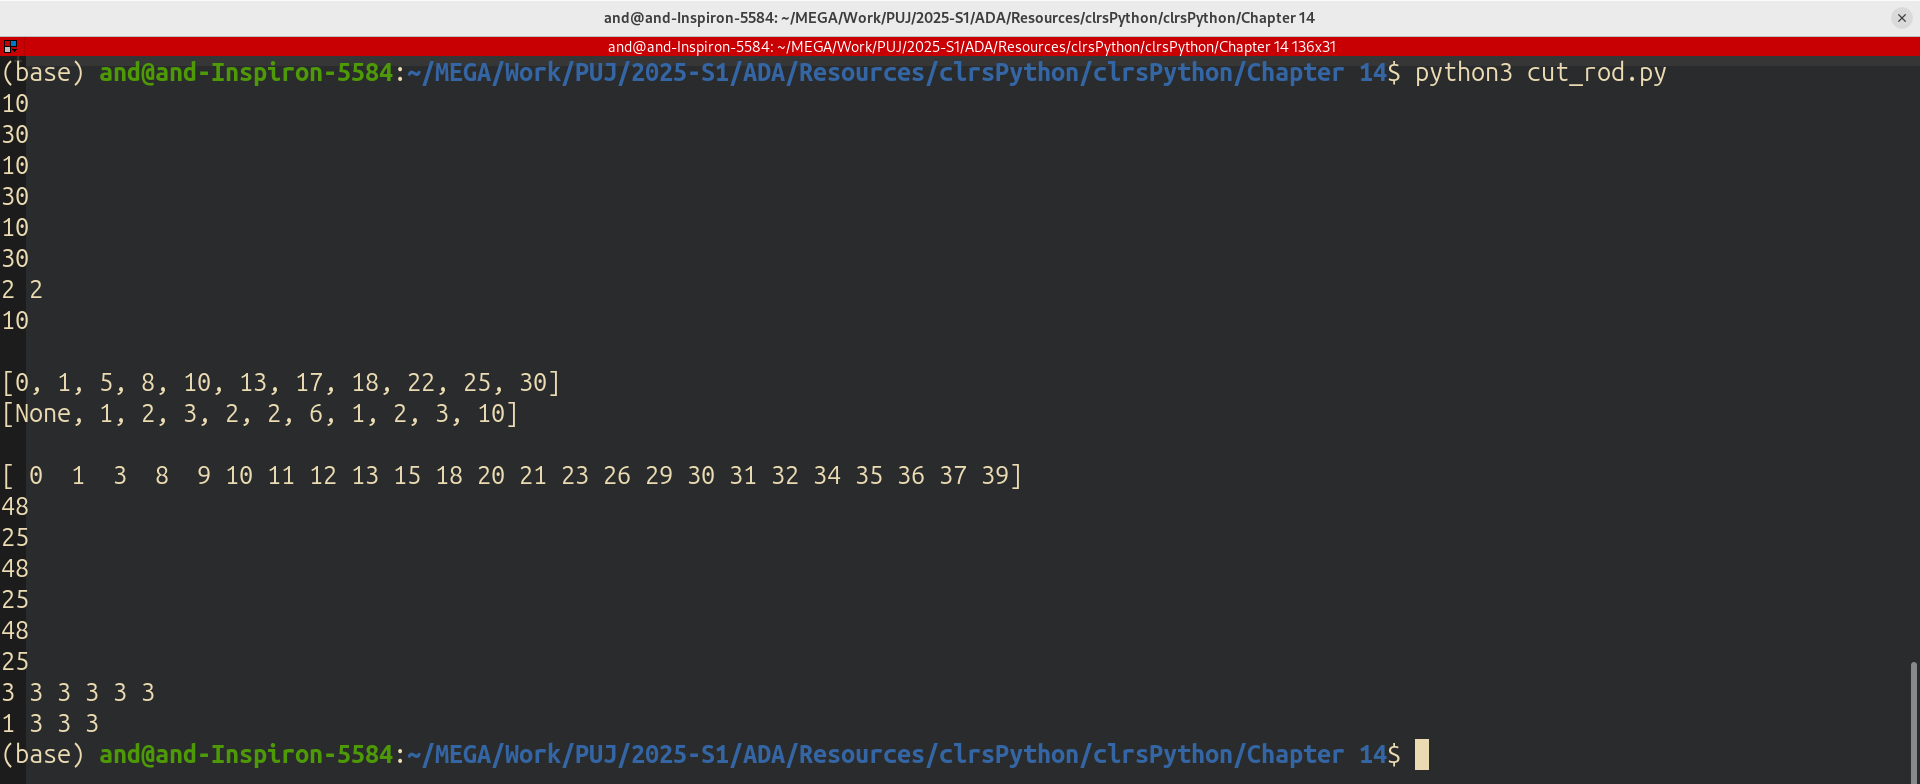
\includegraphics[width=\textwidth]{figures/implementation}
\end{frame}

% \begin{frame}{Learned lessons}
%     \begin{itemize}
%         \item Naive recursive solution has exponential time complexity.
%         \item Dynamic programming reduces it to $\mathcal{O}(n^2)$.
%         \item Optimal substructure and overlapping subproblems make DP suitable.
%     \end{itemize}
% \end{frame}

\section{Matrix-chain multiplication}

\begin{frame}{Matrix-chain multiplication}
    \textbf{Problem}: Given a sequence (chain) $\langle A_1, A_2, \ldots, A_n\rangle$ of $n$ matrices, compute the product $A_1 A_2 \cdots A_n$ using standard matrix multiplication (not Strassen's method) while minimizing the number of scalar multiplications.

    \begin{alertblock}{}
        How to parenthesize the product to minimize the number of scalar multiplications?
    \end{alertblock}
\end{frame}

\begin{frame}{Matrix-chain multiplication}
    For example, if the chain of matrices is $\langle A_1 , A_2 , A_3 , A_4 \rangle$, then you can fully parenthesize the product $A_1 \cdot A_2 \cdot A_3 \cdot A_4$ in five distinct ways:
    \vspace{5mm}

    \centering
    \begin{tabular}{c}
        $(A_1 (A_2 (A_3 A_4)))$, \\
        $(A_1 ((A_2 A_3) A_4))$, \\
        $((A_1 A_2) (A_3 A_4))$, \\
        $((A_1 (A_2 A_3)) A_4)$, \\
        $(((A_1 A_2) A_3) A_4)$ \\
    \end{tabular}
\end{frame}

\begin{frame}{Matrix-chain multiplication}
    The RECTANGULAR-MATRIX-MULTIPLY procedure computes $C = C + A \cdot B$ for three matrices $A = (a_{ij})$, $B = (b_{ij})$, and $C = (c_{ij})$, where $A$ is $p \times q$, $B$ is $q \times r$, and $C$ is $p \times r$.

    \centering
    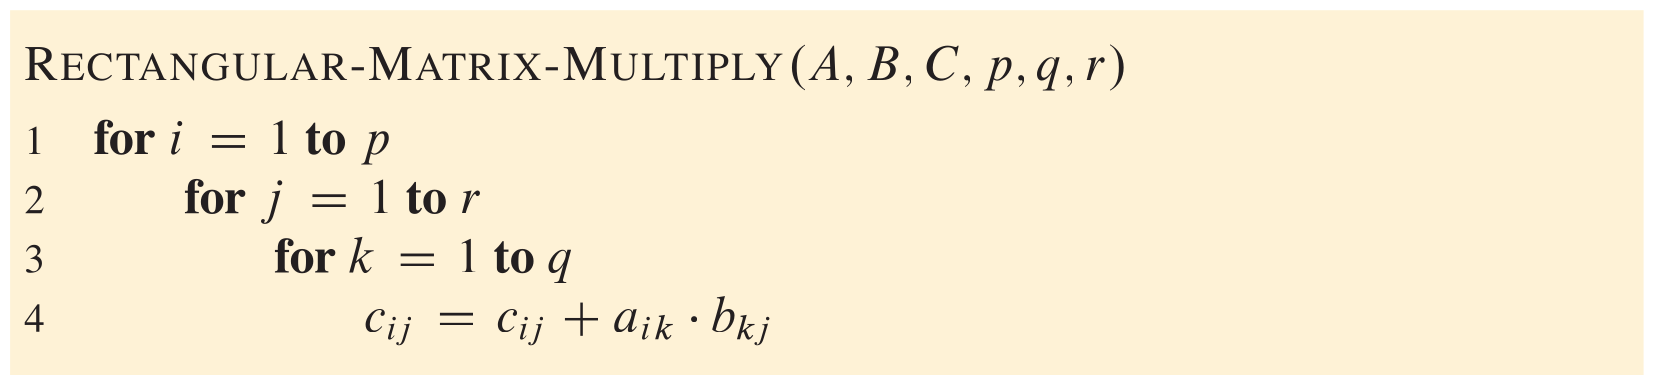
\includegraphics[width=\textwidth]{figures/rmp}
\end{frame}

\begin{frame}{Matrix-chain multiplication}
    \begin{itemize}
        \item Suppose multiplying matrices A and B: $C = A \cdot B$.
        \item The matrices must be compatible: number of columns of $A$ equals number of rows of $B$.
        \item If A is $p \times q$ and B is $q \times r$, then C is $p \times r$ and takes $pqr$ scalar multiplications.
    \end{itemize}
\end{frame}

\begin{frame}{Example}
    $A_1: 10 \times 100$, $A2: 100 \times 5$, $A3: 5 \times 50$. Compute $A_1 A_2 A_3$, which is $10 \times 50$.
    \begin{itemize}
        \item Try parenthesizing by $((A_1 A_2) A_3)$. First perform $10 \times 100 \times 5 = 5000$ multiplications, then perform $10 \times 5 \times 50 = 2500$, for a total of 7500.
        \item Try parenthesizing by $(A_1 (A_2 A_3))$. First perform $100 \times 5 \times 50 = 25,000$ multiplications, then perform $10 \times 100 \times 50 = 50,000$, for a total of 75,000.
        \item The first way is 10 times faster.
    \end{itemize}
\end{frame}

\begin{frame}{Input to the Problem}
    \begin{itemize}
        \item Let $A_i$ be $p_{i - 1} \times p_i$. The input is the sequence of dimensions $\langle p_0, p_1, p_2, \ldots , p_n \rangle$.
        \item \textbf{Note}: Not actually multiplying matrices. Just deciding an order with the lowest cost.
    \end{itemize}
\end{frame}

\begin{frame}{Counting the Number of Parenthesizations}
    \begin{itemize}
        \item Let $P(n)$ denote the number of ways to parenthesize a product of $n$ matrices. $P(1) = 1$.
        \item When $n \geq 2$, can split anywhere between $A_k$ and $A_{k + 1}$ for $k = 1, 2, \ldots, n - 1$. Then have to split the subproducts.
        \item Get
            \begin{equation*}
                \begin{align*}
                    P(n) =
                        \begin{cases}
                            1 & \text{ if } n = 1 \text{, } \\
                            \sum_{k = 1}^{n - 1} P(k)P(n - k) & \text{ if } n \geq 2 \text{.}
                        \end{cases}
                \end{align*}
            \end{equation*}
        \item The solution is $P(n) = \Omega \left( \frac{4^n}{n^{\frac{3}{2}}} \right)$. So brute force is a bad strategy.
    \end{itemize}
\end{frame}

\begin{frame}{Step 1: Structure of an optimal solution}
    \begin{itemize}
        \item Let $A_{i:j}$ be the matrix product $A_i A_{i+1} \cdots A_j$.
        \item If $i < j$, then must split between $A_k$ and $A_{k+1}$ for some $i \leq k < j \Rightarrow$  compute $A_{i:k}$ and $A_{k+1:j}$ and then multiply them together.
        \item Cost is
            \begin{equation*}
                \begin{align*}
                        & \text{ cost of computing } A_{i:k} \\
                    +   & \text{ cost of computing } A_{k+1:j} \\
                    +   & \text{ cost of multiplying them together.}
                \end{align*}
            \end{equation*}
    \end{itemize}
\end{frame}

\begin{frame}{Optimal substructure}
    \begin{itemize}
        \item Suppose that optimal parenthesization of $A_{i:j}$ splits between $A_k$ and $A_{k+1}$.
        \item Then the parenthesization of $A_{i:k}$ must be optimal.
        \item Otherwise, if there's a less costly way to parenthesize it, you'd use it and get a parenthesization of $A_{i:j}$ with a lower cost. Same for $A_{k+1:j}$.
        \item Therefore, to build an optimal solution to $A_{i:j}$:
            \begin{itemize}
                \item split it into how to optimally parenthesize $A_{i:k}$ and $A_{k+1:j}$,
                \item find optimal solutions to these subproblems,
                \item and then combine the optimal solutions.
            \end{itemize}
        \item Need to consider all possible splits.
    \end{itemize}
\end{frame}

\begin{frame}{Step 2: A recursive solution}
    \begin{itemize}
        \item Define the cost of an optimal solution recursively in terms of optimal subproblem solutions.
        \item Let $m[i, j]$ be the minimum number of scalar multiplications to compute $A_{i:j}$. For the full problem, want $m[1, n]$.
        \begin{itemize}
            \item If $i = j$, then just one matrix $ m[i, i] = 0$ for $i = 1, 2, \ldots, n$.
            \item If $i < j$, then suppose the optimal split is between $A_k$ and $A_{k+1}$, where $i \leq k < j$.
            \item Then $m[i, j] = m[i, k] + m[k+1, j] + p_{i-1} p_k p_j$.
        \end{itemize}
    \end{itemize}
\end{frame}

\begin{frame}{Step 2: A recursive solution}
    \begin{itemize}
        \item But that's assuming you know the value of $k$. Have to try all possible values and pick the best, so that
            \begin{equation*}
                \scriptsize
                \begin{align*}
                    m[i, j] =
                        \begin{cases}
                            0 & \text{ if } i = j \text{,} \\
                            min \{ m[i, k] + m[k+1, j] + p_{i-1} p_k p_j : i \leq k < j \} & \text{ if } i < j \text{.}
                        \end{cases}
                \end{align*}
            \end{equation*}
        \item That formula gives the cost of an optimal solution, but not how to construct it.
            \begin{itemize}
                \item Define $s[i, j]$ to be a value of $k$ to split $A_{i:j}$ in an optimal parenthesization.
                \item Then $s[i; j] = k$ such that $m[i, j] = m[i, k] + m[k+1, j] + p_{i-1} p_k p_j$.
            \end{itemize}
    \end{itemize}
\end{frame}

\begin{frame}{Step 3: Compute the optimal costs}
    \begin{itemize}
        \item Could implement a recursive algorithm based on the above equation for $m[i, j]$ but it would take exponential time.
        \item There are not all that many distinct subproblems:
            \begin{itemize}
                \item just one for each $i, j$ such that $1 \leq i \leq j \leq n$.
                \item there are ${n \choose 2} + n = \Theta (n^2)$ of them.
                \item thus, a recursive algorithm would solve the same subproblem over and over.
            \end{itemize}
        \item In other words, this problem has overlapping subproblems.
    \end{itemize}
\end{frame}

\begin{frame}{Step 3: Compute the optimal costs}
    \begin{itemize}
        \item Here is a tabular, bottom-up method to solve the problem.
        \item It solves subproblems in order of increasing chain length.
    \end{itemize}
    \centering
    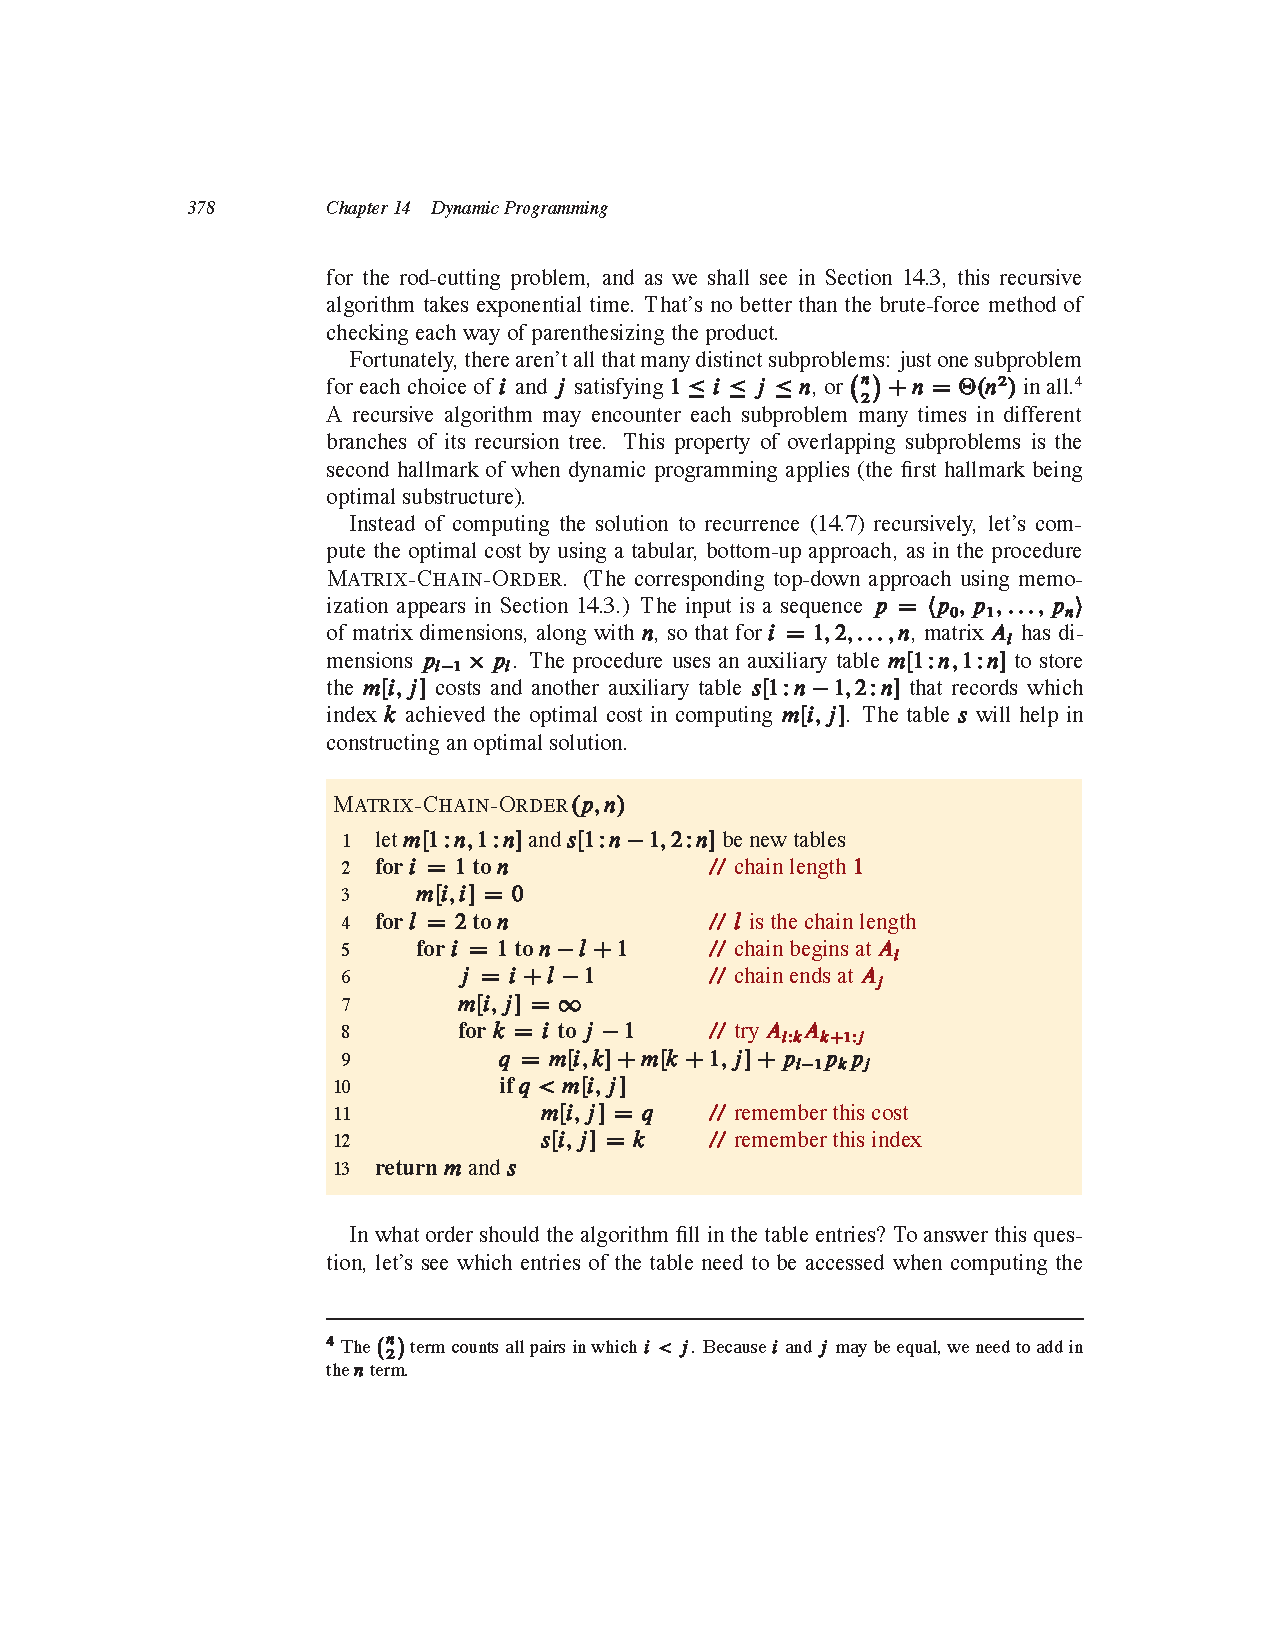
\includegraphics[width=0.7\textwidth, trim={5cm 7.5cm 4cm 13cm}, clip]{figures/p378} \\ \pause
    \textbf{Time}: $O(n^3)$, from triply nested loops. Also $\Omega (n^3) \Rightarrow \Theta (n^3)$.
\end{frame}

\begin{frame}{Step 4: Construct an optimal solution}
    \begin{itemize}
        \item With the $s$ table filled in, recursively print an optimal solution.
        \item Initial call is \textsc{Print-Optimal-Parens}$(s, 1, n)$.
    \end{itemize}
    \vspace{5mm}

    \centering
    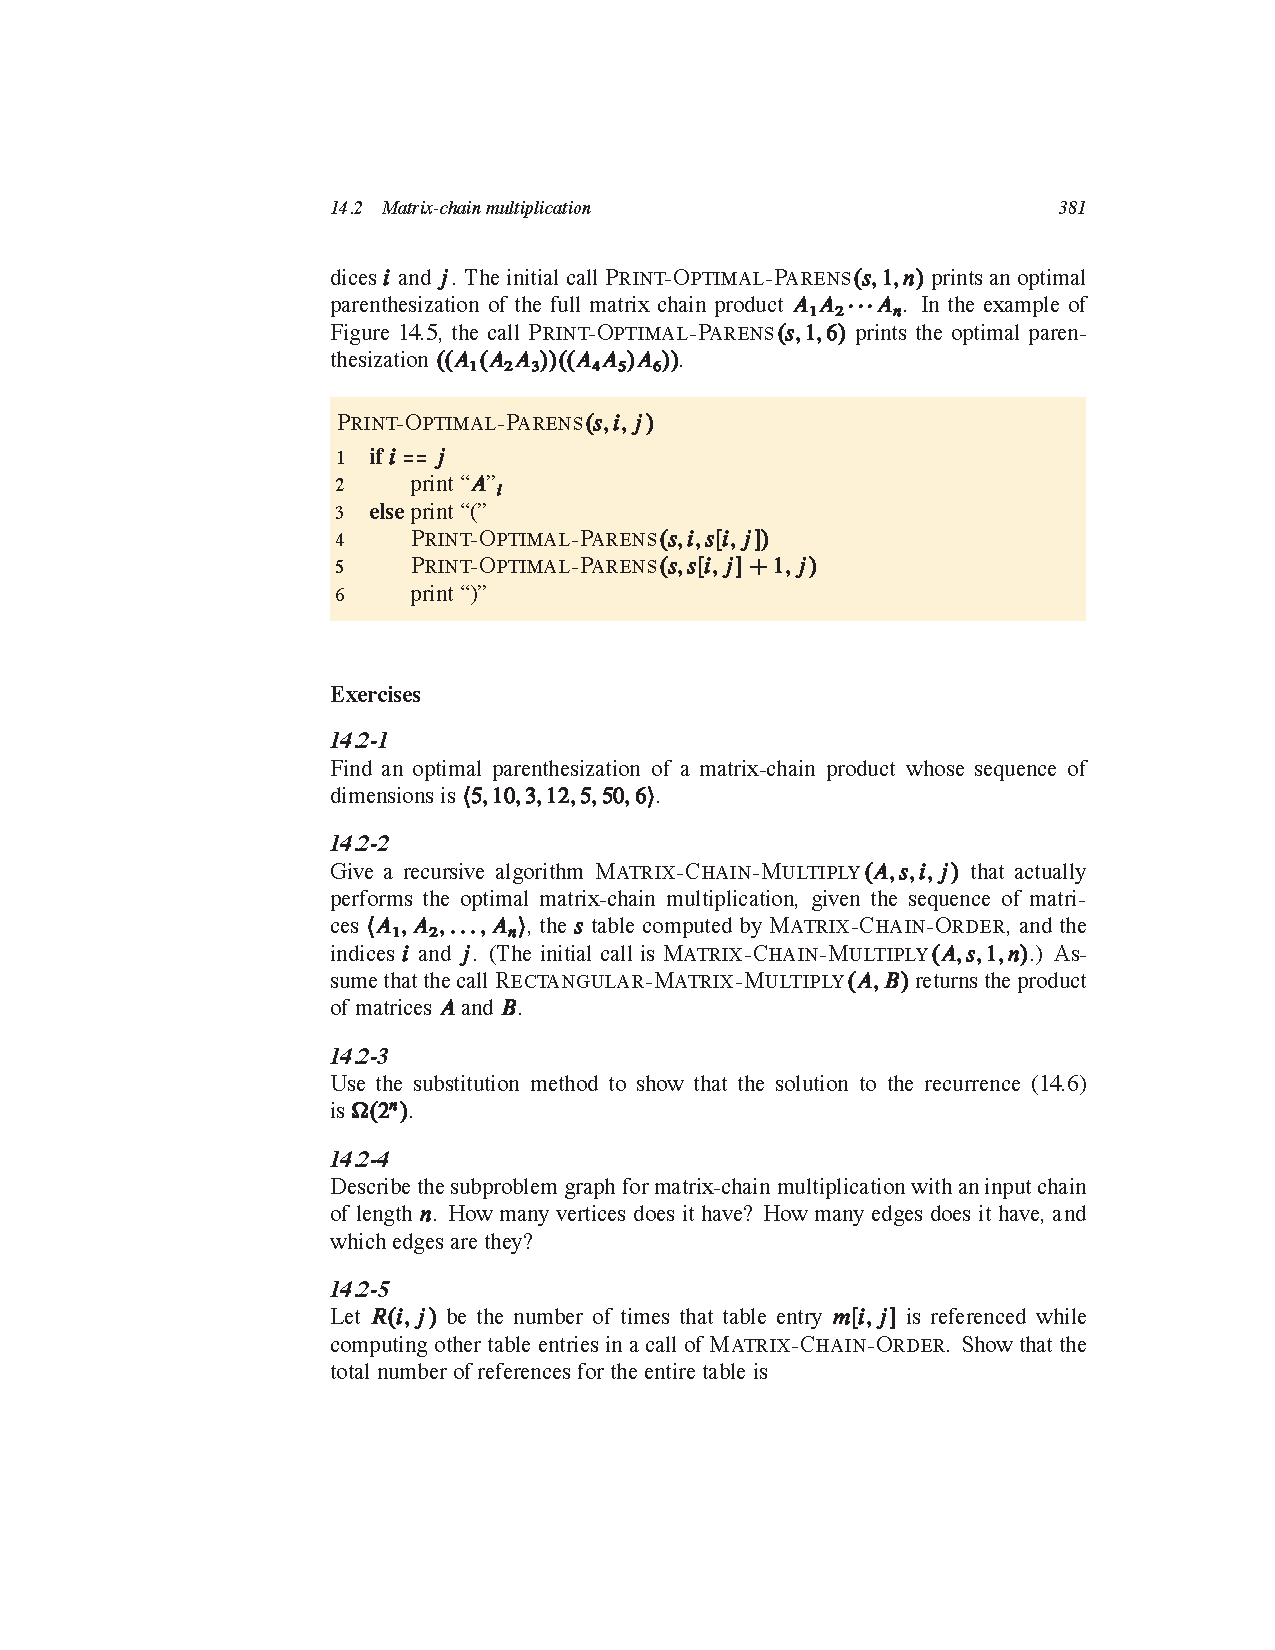
\includegraphics[width=0.9\textwidth, trim={4cm 17cm 5cm 6.75cm}, clip]{figures/p381}
\end{frame}

\begin{frame}{Example}
    \centering
    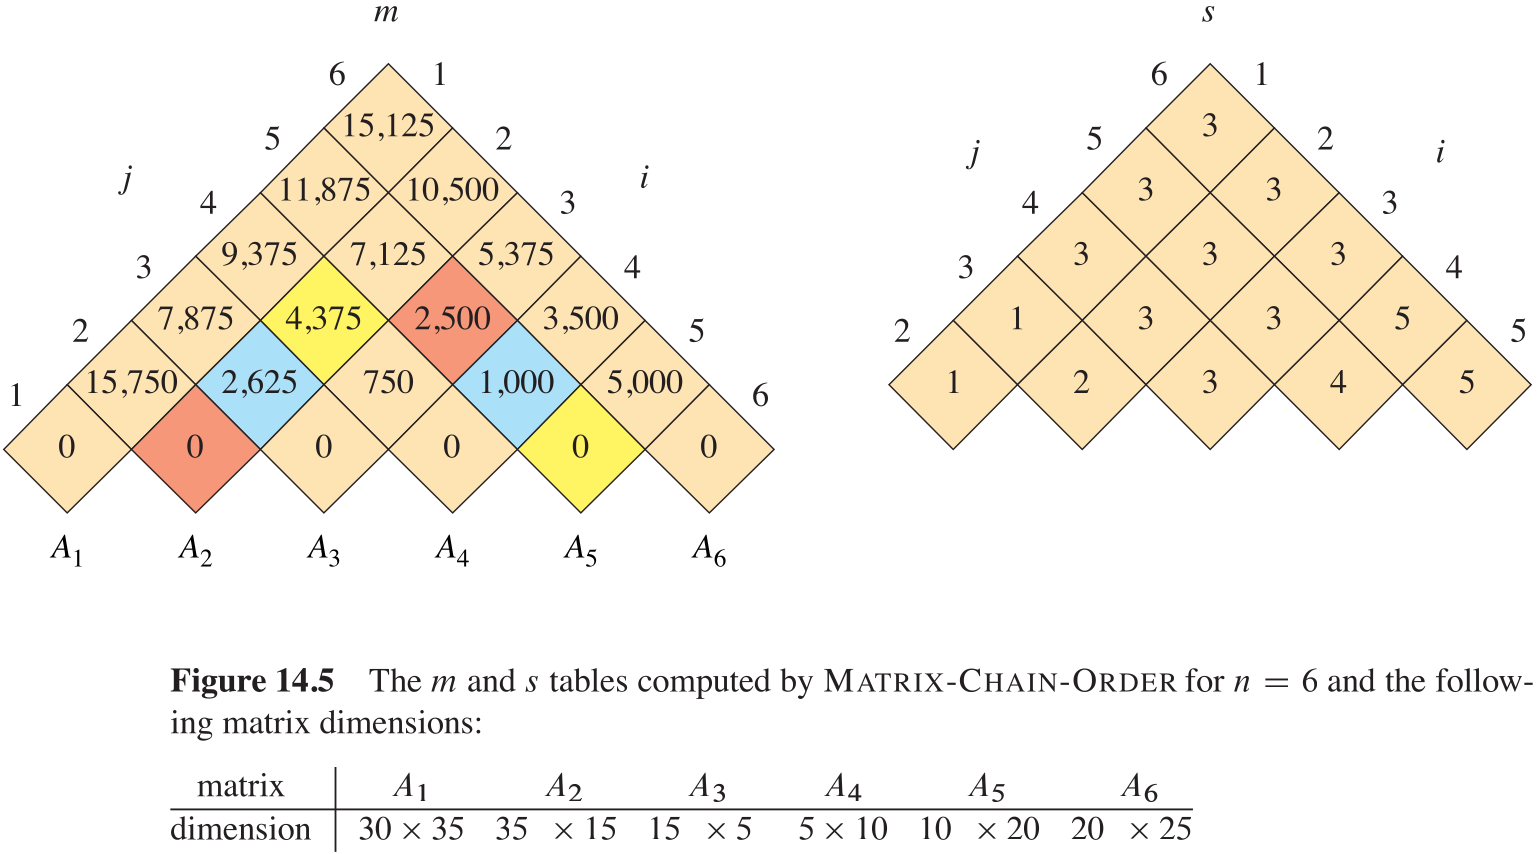
\includegraphics[width=0.9\textwidth]{figures/rmp2}
\end{frame}

\begin{frame}{Code Implemantation}
    \centering
    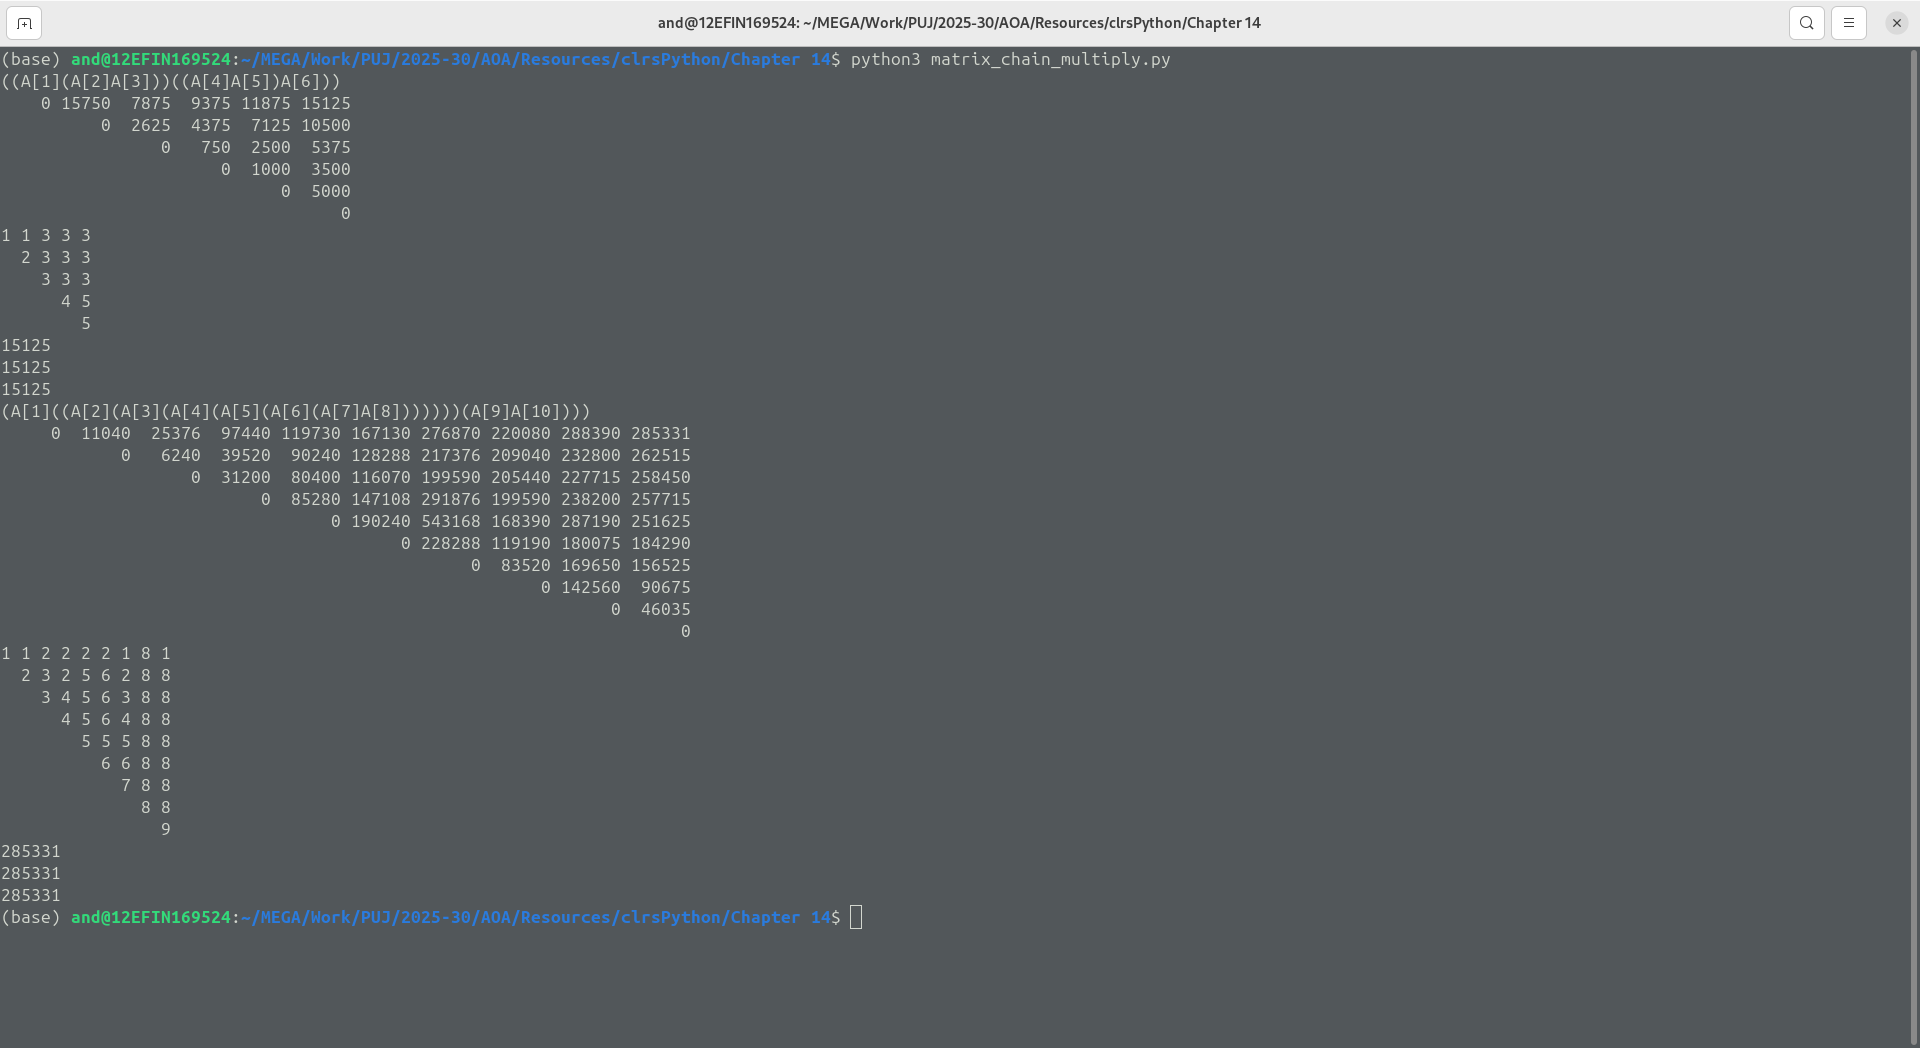
\includegraphics[width=\textwidth]{figures/matrix_chain_multiplication}
\end{frame}

\section{Optimal binary search trees}

\begin{frame}{Optimal binary search trees}
    \begin{itemize}
        \item Given sequence $K = \langle k_1, k_2, \ldots, k_n \rangle$ of $n$ distinct keys, sorted $(k_1 < k_2 < \ldots < k_n)$.
        \item Want to build a binary search tree from the keys.
        \item For $k_i$, have probability $p_i$ that a search is for $k_i$.
        \item Want BST with minimum expected search cost.
    \end{itemize}
\end{frame}

\begin{frame}{BST Cost}
    Actual cost = \# of items examined.
    \begin{center}
        \footnotesize
        For $k_i$, $cost = depth_T (k_i) + 1$, where $depth_T (k_i) =$ depth $k_i$ in BST $T$.
    \end{center}
    $E[$ search cost in $T]$
    \begin{equation*}
        \begin{align*}
            =& \sum_{i=n}^{n} (depth_T(k_i) + 1) \cdot p_i \\
            =& \sum_{i=n}^{n} depth_T(k_i) \cdot p_i + \sum_{i=1}^{n} p_i \\
            =& 1 + \sum_{i=n}^{n} depth_T(k_i) \cdot p_i
        \end{align*}
    \end{equation*}
\end{frame}

\begin{frame}{Example}
    \centering
    \begin{tabular}{c | c c c c c}
        i & 1 & 2 & 3 & 4 & 5 \\
        \hline
        $p_i$ & .25 & .2 & .05 & .2 & .3
    \end{tabular}
    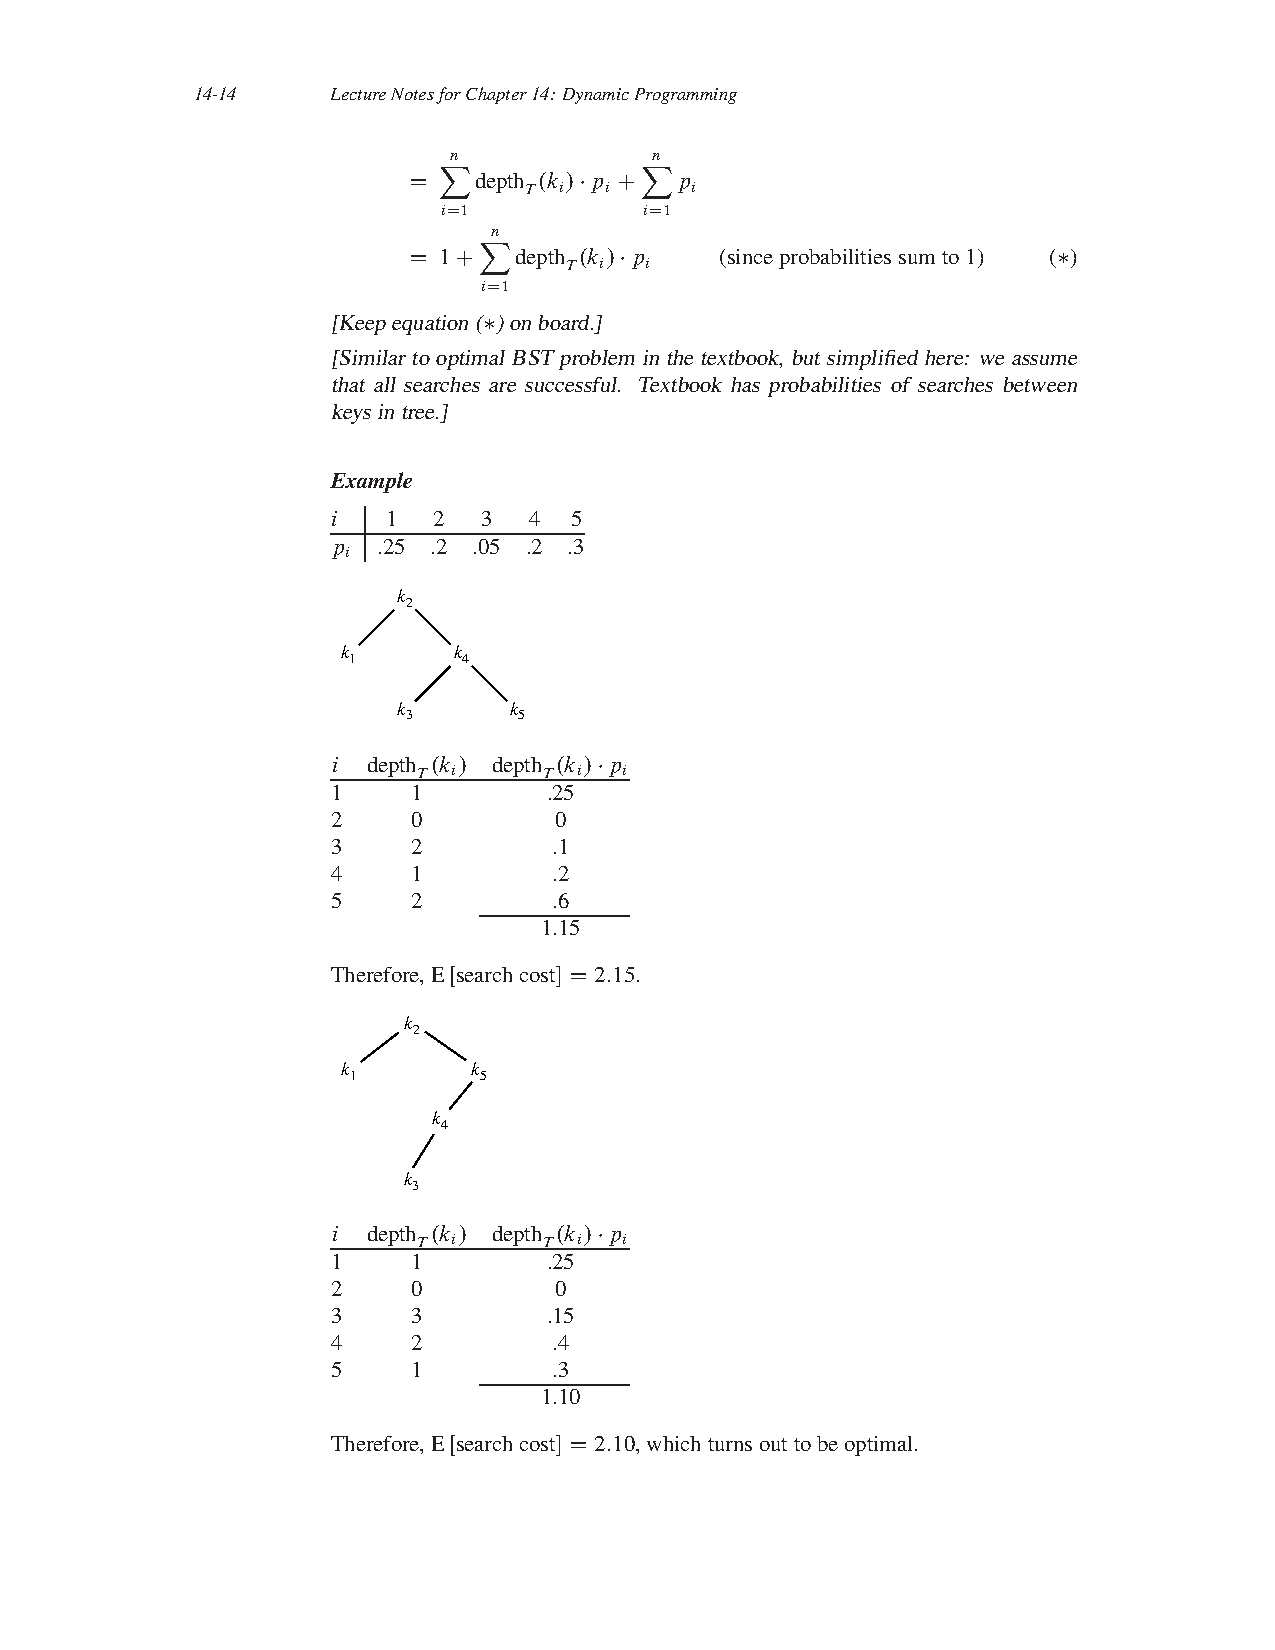
\includegraphics[width=0.8\textwidth, trim={4cm 12cm 4cm 9.75cm}, clip]{figures/BST_example}
    \begin{itemize}
        \item Therefore, E[search cost] = 2.15.
    \end{itemize}
\end{frame}

\begin{frame}{Example}
    \centering
    \begin{tabular}{c | c c c c c}
        i & 1 & 2 & 3 & 4 & 5 \\
        \hline
        $p_i$ & .25 & .2 & .05 & .2 & .3
    \end{tabular}
    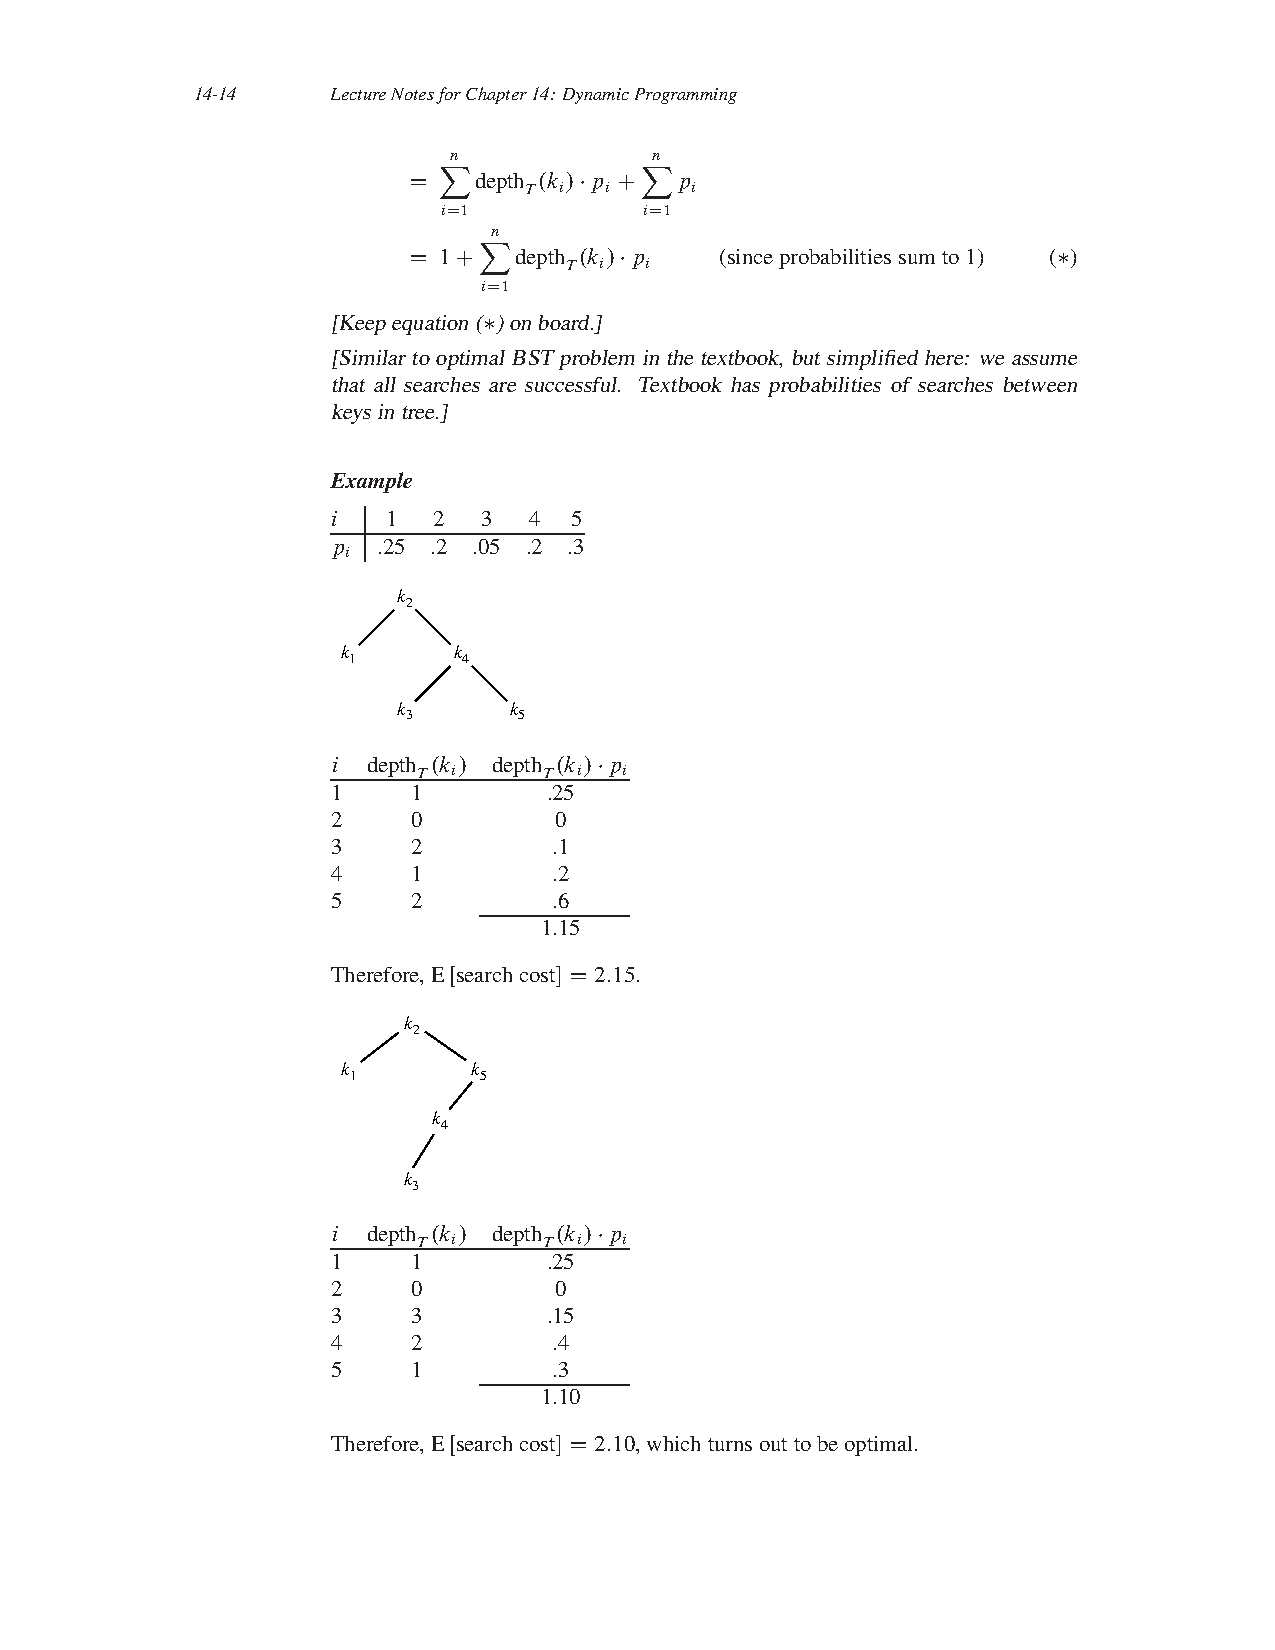
\includegraphics[width=0.8\textwidth, trim={4cm 4cm 4cm 17cm}, clip]{figures/BST_example}
    \begin{itemize}
        \item Therefore, E[search cost] = 2.10, which turns out to be optimal.
    \end{itemize}
\end{frame}

\begin{frame}{Observations}
    \begin{itemize}
        \item Optimal BST might not have smallest height.
        \item Optimal BST might not have highest-probability key at root.
    \end{itemize}
    Build by exhaustive checking?
    \begin{itemize}
        \item Construct each $n$-node BST.
        \item For each, put in keys.
        \item Then compute expected search cost.
        \item But there are $\Omega \left( \frac{4^n}{n^{\frac{3}{2}}} \right)$ different BSTs with $n$ nodes.
    \end{itemize}
\end{frame}

\begin{frame}{Step 1: The structure of an optimal BST}
    Consider any subtree of a BST.  It contains keys in a contiguous range $k_i, \ldots, k_j$ for some $1 \leq i \leq j \leq n$.

    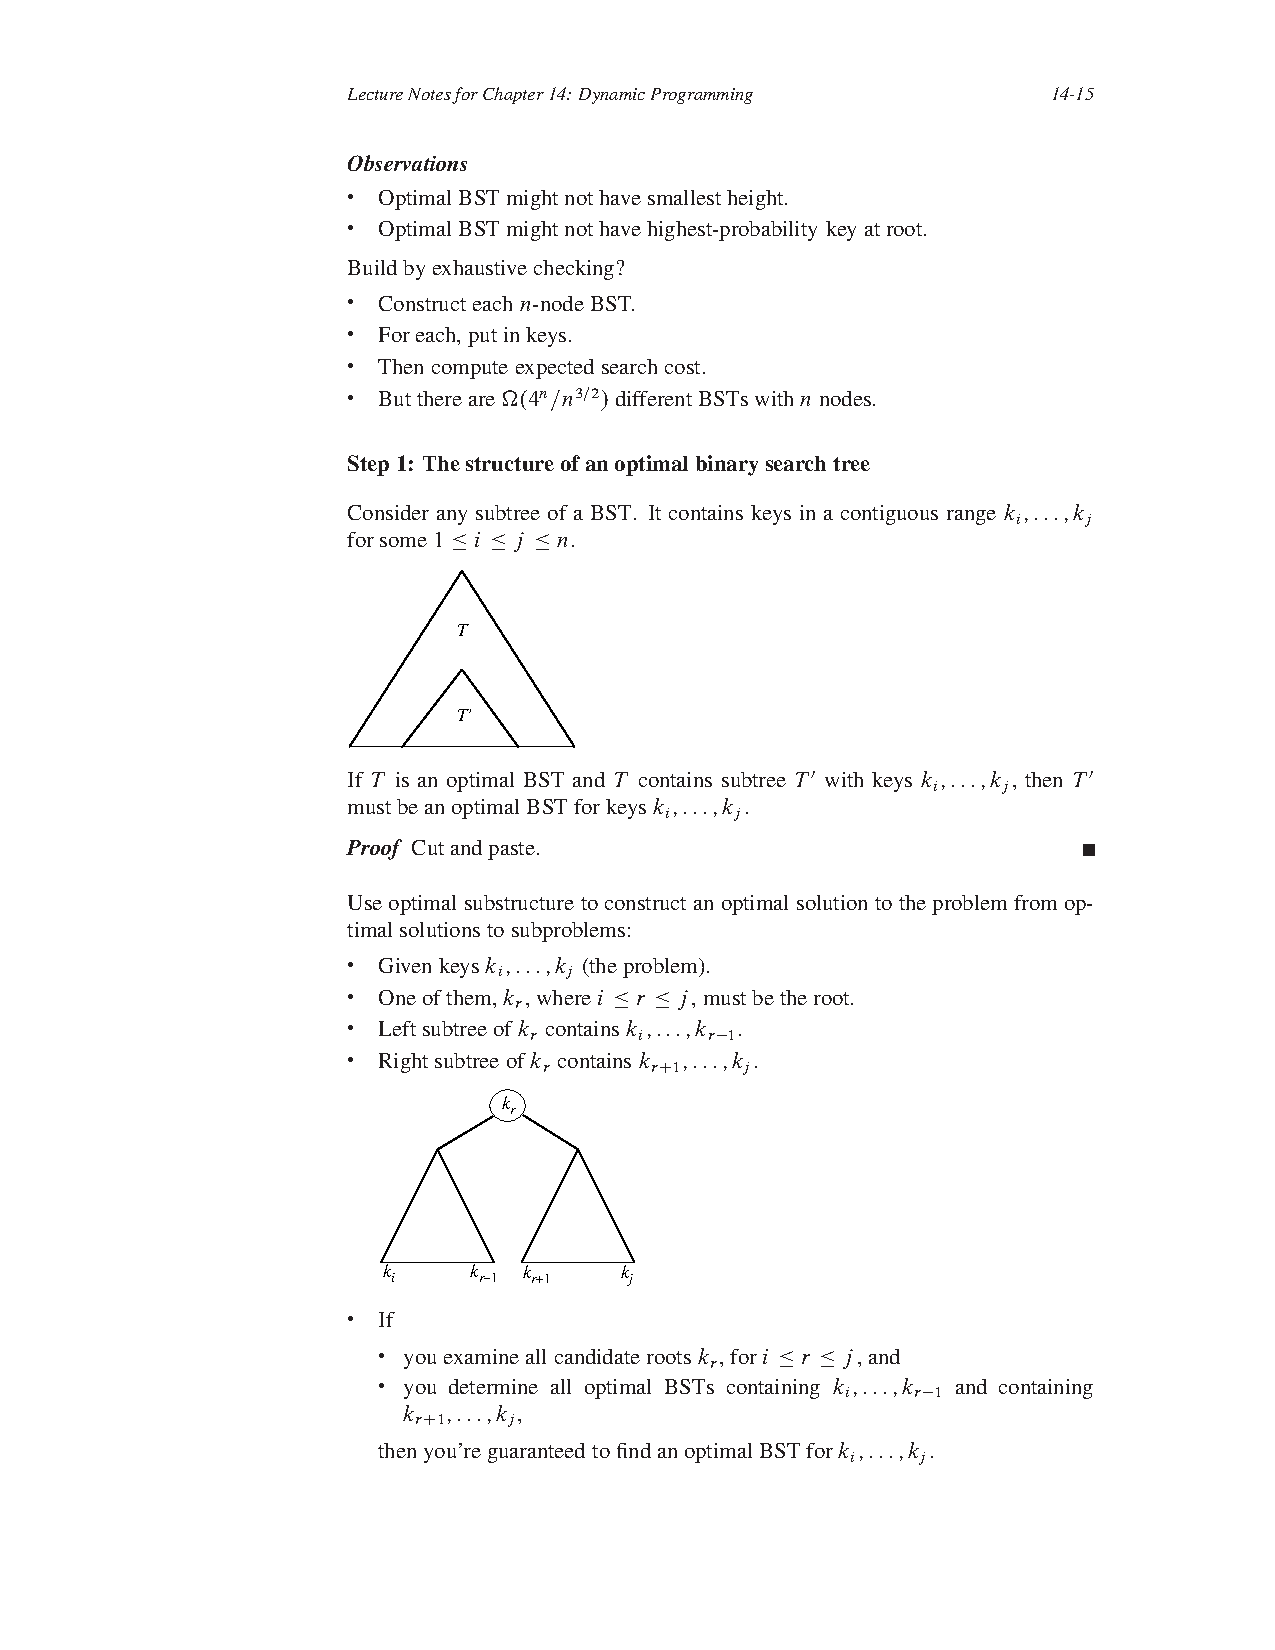
\includegraphics[width=\textwidth, trim={4cm 15cm 4cm 9.5cm}, clip]{figures/BST_step1}

    If $T$ is an optimal BST and $T$ contains subtree $T^\prime$ with keys $k_i, \ldots, k_j$, then $T^\prime$ must be an optimal BST for keys $k_i, \ldots, k_j$.
\end{frame}

\begin{frame}{Step 1: The structure of an optimal BST}
    Use optimal substructure to construct an optimal solution to the problem from optimal solutions to subproblems:
    \begin{itemize}
        \item Given keys $k_i, \ldots, k_j$ (the problem).
        \item One of them, $k_r$, where $i \leq r \leq j$, must be the root.
        \item Left subtree of $k_r$ contains $k_i, \ldots, k_{r-1}$.
        \item Right subtree of $k_r$ contains $k_{r+1}, \dots, k_j$.
    \end{itemize}
    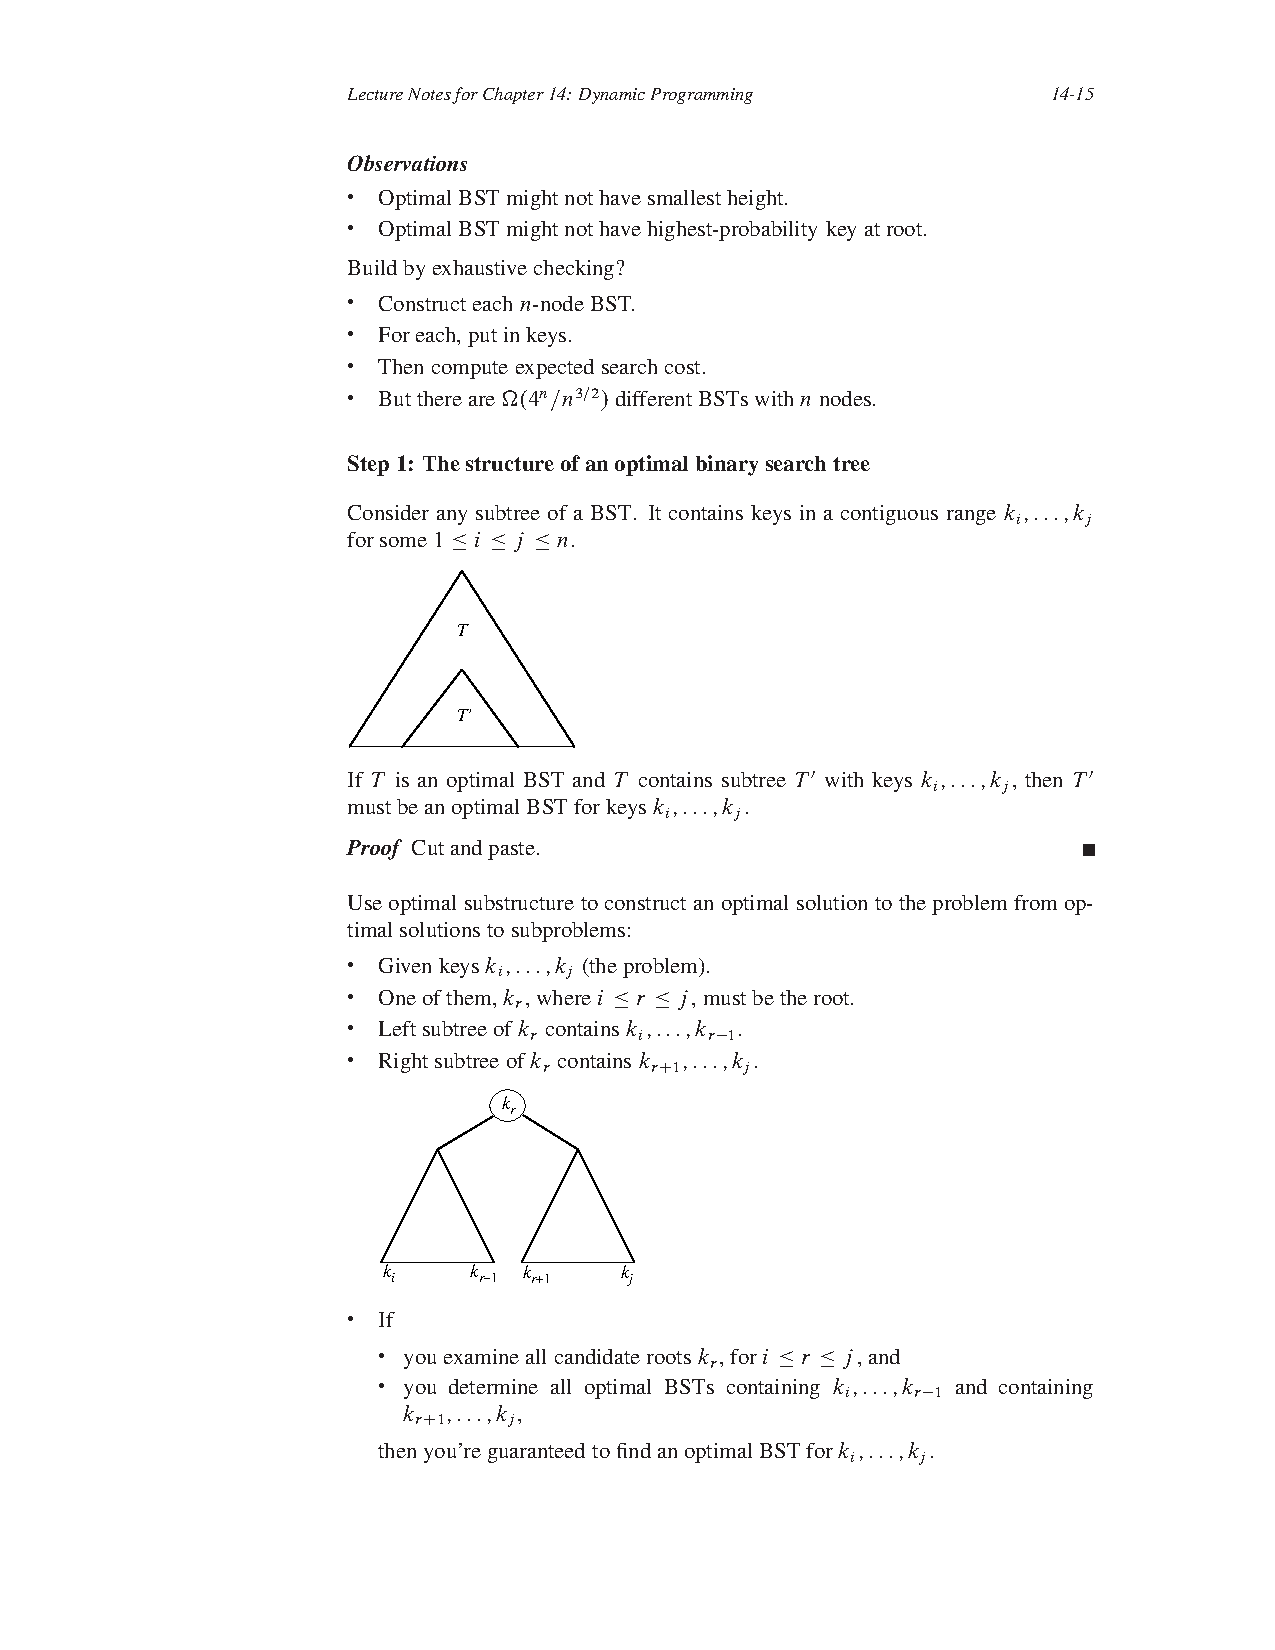
\includegraphics[width=\textwidth, trim={4cm 6cm 4cm 18.25cm}, clip]{figures/BST_step1}
\end{frame}

\begin{frame}{Step 1: The structure of an optimal BST}
    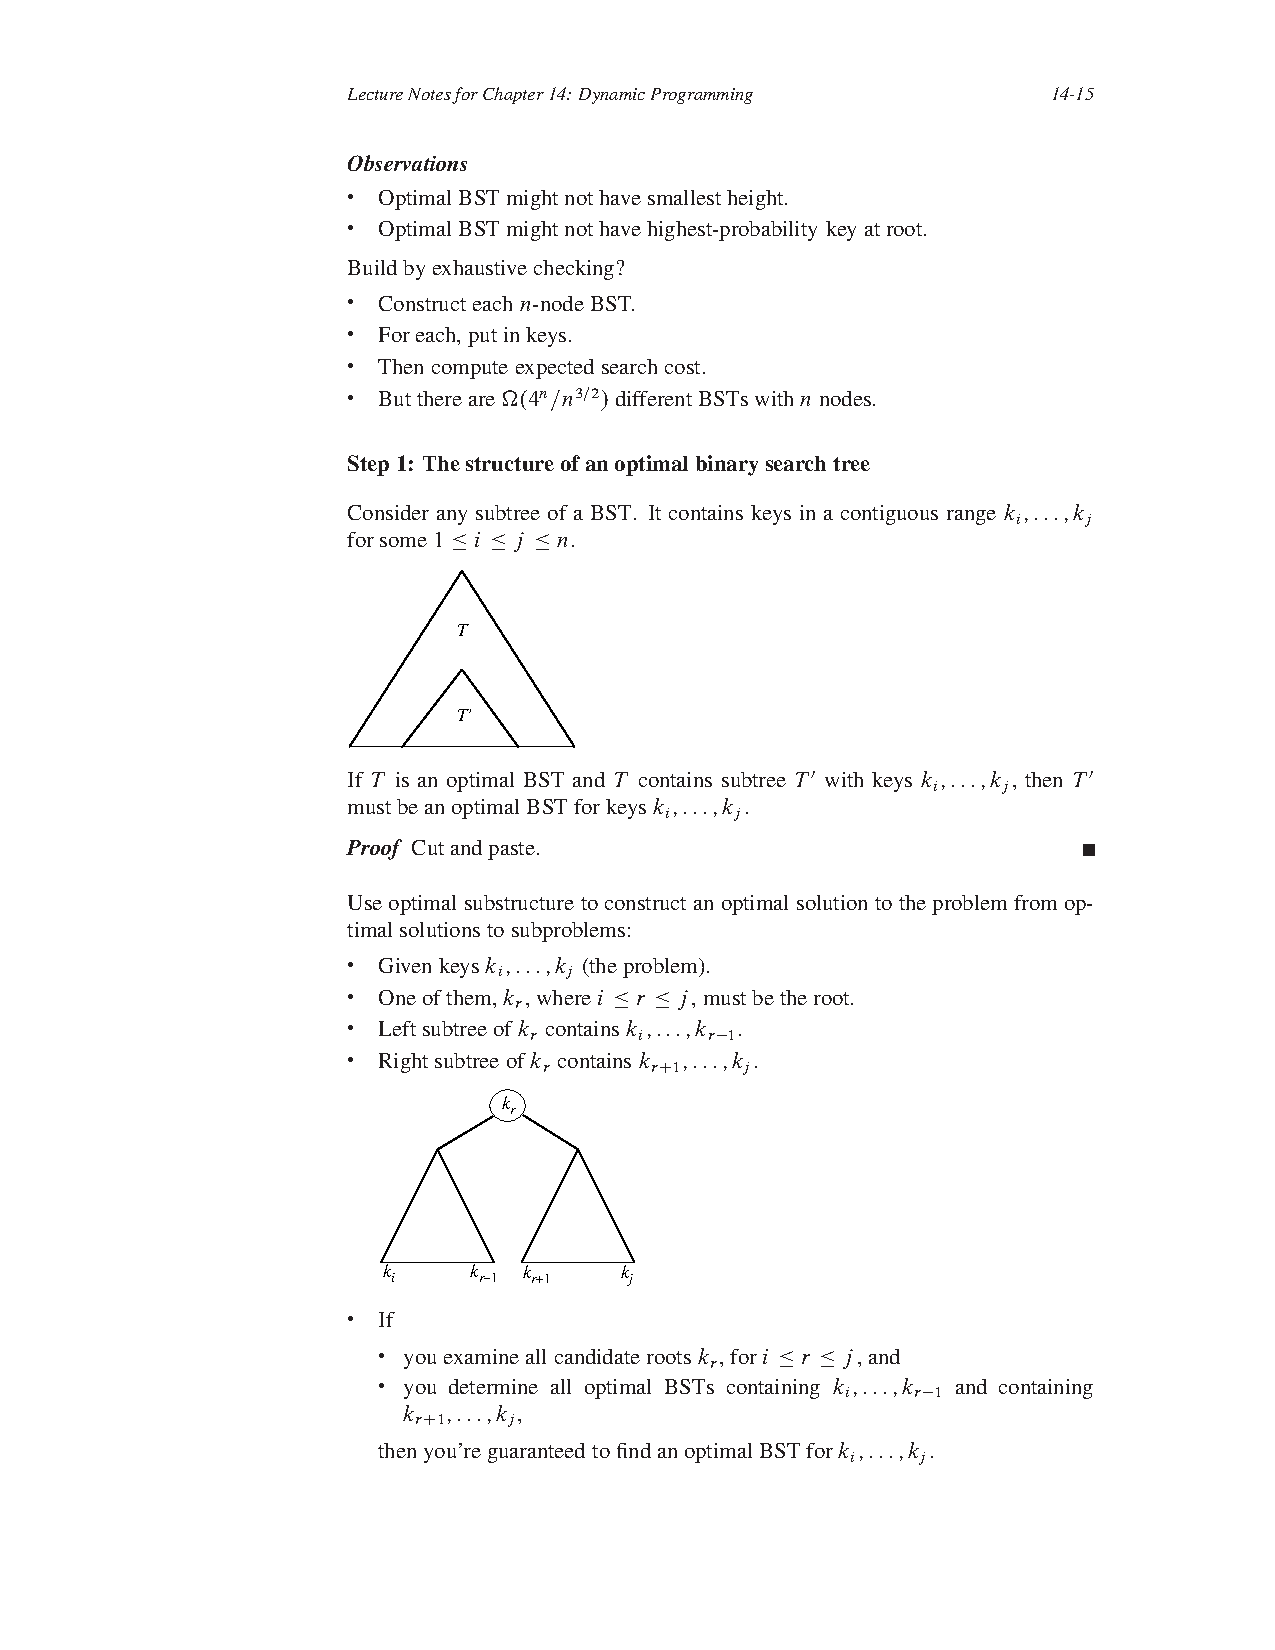
\includegraphics[width=\textwidth, trim={4cm 6cm 4cm 18.25cm}, clip]{figures/BST_step1}
    \begin{itemize}
        \item If
            \begin{itemize}
                \item you examine all candidate roots $k_r$, for $i \leq r \leq j$, and
                \item you determine all optimal BSTs containing $k_i, \ldots, k_{r-1}$ and containing $k_{r+1}, \ldots, k_j$,
            \end{itemize}
        then you're guaranteed to find an optimal BST for $k_i, \ldots, k_j$.
    \end{itemize}
\end{frame}

\begin{frame}{Step 2: Recursive solution}
    Subproblem domain:
    \begin{itemize}
        \item Find optimal BST for $k_i, \ldots, k_j$, where $i \geq 1$, $j \leq n$, $j \geq i - 1$.
        \item When $j = i - 1$, the tree is empty.
    \end{itemize}
    Define $e[i, j] = $ expected search cost of optimal BST for $k_i, \dots, k_j$.
\end{frame}

\begin{frame}{Step 2: Recursive solution}
    \begin{itemize}
        \item If $j = i - 1$, then $e[i, j] = 0$.
        \item If $j \geq i$,
            \begin{itemize}
                \item Select root $k_r$, for some $i \leq r \leq j$.
                \item Make an optimal BST with $k_i, \ldots, k_{r-1}$ as the left subtree.
                \item Make an optimal BST with $k_{r+1}, \ldots, k_j$ as the right subtree.
                \item Note: when $r = i$, left subtree is $k_i, \dots, k_{i-1}$; when $r = j$, right subtree is $k_{j+1}, \ldots, k_j$.  These subtrees are empty.
            \end{itemize}
    \end{itemize}
\end{frame}

\begin{frame}{Step 2: Recursive solution}
    When a subtree becomes a subtree of a node:
    \begin{itemize}
        \item Depth of every node in subtree goes up by 1.
        \item Expected search cost increases by
            \begin{equation*}
                \begin{align*}
                    w(i, j) = \sum_{l = i}^{j} p_l
                \end{align*}
            \end{equation*}
    \end{itemize}
    If $k_r$ is the root of an optimal BST for $k_i, \ldots, k_j$:
        \begin{equation*}
            \begin{align*}
                e[i, j] = p_r + (e[i, r-1] + w(i, r-1)) + (e[r+1, j] + w(r+1, j))
            \end{align*}
        \end{equation*}
    \begin{itemize}
        \item But $w(i, j) = w(i, r-1) + p_r + w(r+1, j)$.
        \item Therefore, $e[i, j] = e[i,r-1] + e[r+1, j] + w(i, j)$
    \end{itemize}
\end{frame}

\begin{frame}{Step 2: Recursive solution}
    That equation assumes that we already know which key is $k_r$.  We don’t.
    \begin{itemize}
        \item Try all candidates, and pick the best one:
            \begin{equation*}
                \scriptsize
                \begin{align*}
                    e[i, j] =
                        \begin{cases}
                            0 & \text{ if } j = i - 1 \text{,} \\
                            \min \left \{ e[i, r-1] + e[r+1, j] + w(i, j):i \leq r \leq j \right \} & \text{ if } i \leq j \text{.}
                        \end{cases}
                \end{align*}
            \end{equation*}
        \item Could write a recursive algorithm\ldots
        \item Have a look at this \href{https://www.youtube.com/watch?v=Tw1k46ywN6E}{lecture}\footnote{Watch from minute 22:53 til 54:21.}\ldots
    \end{itemize}
\end{frame}


\begin{frame}{}
    \centering
    \Huge End of Lecture 5.
\end{frame}

\section*{Takeaways}

% Tim Duncan's Top 5 Fundamental Takeaways of the Today's Class
\begin{frame}{TDT5FTOTTC}
    \centering
    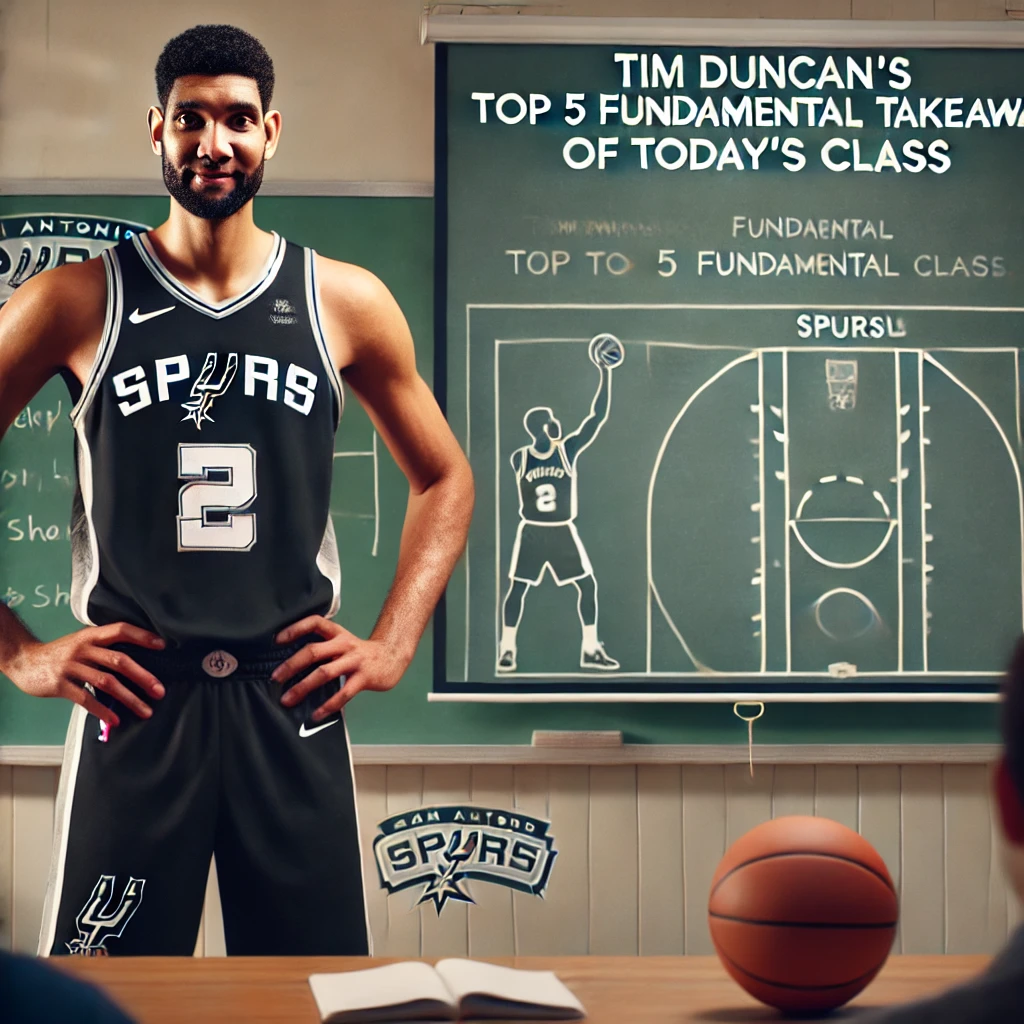
\includegraphics[width=0.55\textwidth]{figures/tim.png}
\end{frame}

\begin{frame}{Top 5 Fundamental Takeaways}
    \small
    \begin{enumerate} \pause

        \item[5] Computing Fibonacci numbers or finding the longest palindromic subsequence becomes efficient when subproblem results are cached to prevent repeated computation. \pause

        \item[4] The LCS problem uses a table-based approach to find the length and content of the longest common subsequence in quadratic time. \pause

        \item[3] DP Has Four Key Steps: identifying the structure, defining recurrence, computing solutions bottom-up, and reconstructing the optimal result. \pause

        \item[2] DP optimizes problems that have \textbf{overlapping subproblems} and \textbf{optimal substructure}. \pause

        \item[1] Dynamic Programming = recursion + memoization.
    \end{enumerate}
\end{frame}

\begin{frame}{Introduction to Algorithms}
    \centering
    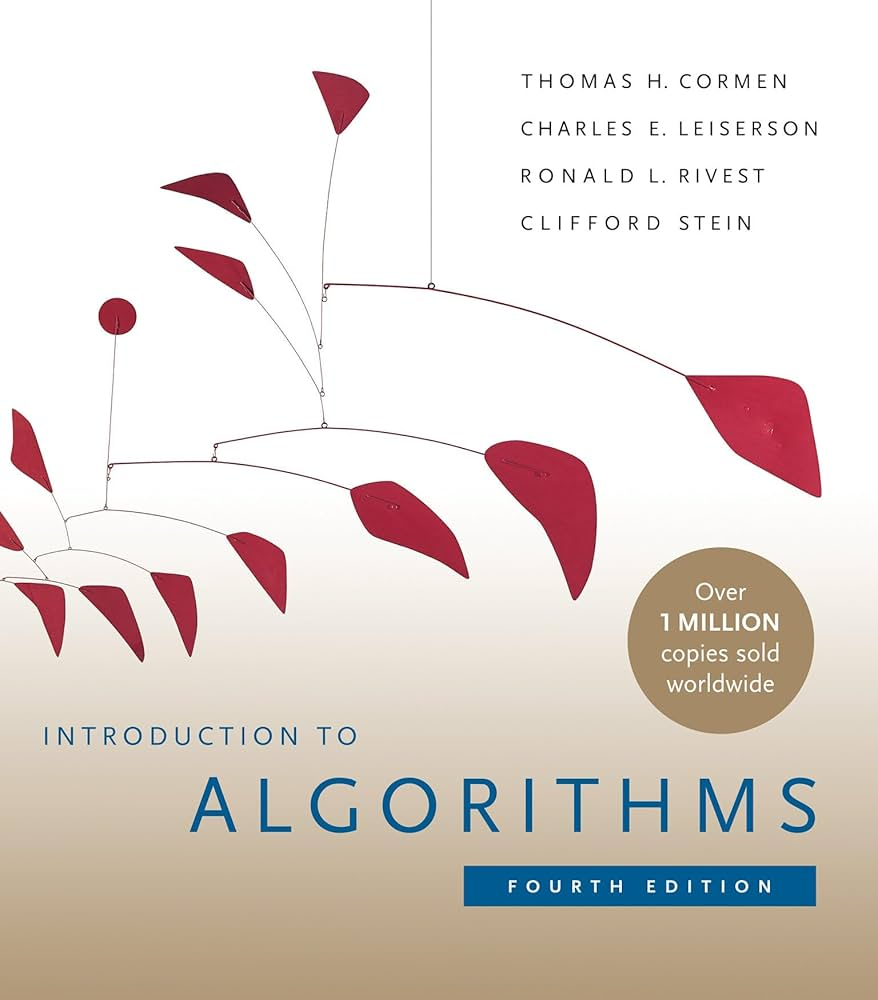
\includegraphics[width=0.35\textwidth]{figures/book_cover.jpg} \\
    \vspace{5mm}{
        \tiny
        Content has been extracted from \textit{Introduction to Algorithms}, Fourth Edition, by Cormen, Leiserson, Rivest, and Stein. MIT Press. 2022.\\
        Visit \url{https://mitpress.mit.edu/9780262046305/introduction-to-algorithms/}.\\
        Original slides from \textit{Introduction to Algorithms 6.046J/18.401J}, Fall 2005 Class by Prof. Charles Leiserson and Prof. Erik Demaine. MIT OpenCourseWare Initiative available at \url{https://ocw.mit.edu/courses/6-046j-introduction-to-algorithms-sma-5503-fall-2005/}.\\
    }
\end{frame}

\end{document}
